% name: MFEFormulary.tex
% date: 10 Jan 14
% auth: Zach Hartwig and Yuri Podpaly
%
% desc: This is the top-level LaTeX file for the Magnetic Fusion
%       Energy Formulary. All required packages, options, commands,
%       and so forth are defined here. Each chapter is split into
%       seperate *.tex files that are included via standard LaTeX
%       commands. Finally, this file also controls building the index
%       and bibliography.

\documentclass[11pt]{book}
\usepackage{enumerate}
\usepackage{amsmath} 
\usepackage{amssymb} 
\usepackage{amsbsy}
\usepackage{graphicx}
\usepackage{graphics}
\usepackage{multirow}
\usepackage{hyperref}
\usepackage{longtable}
\usepackage{makeidx}
\usepackage{float}
\usepackage{caption}
\usepackage{fix-cm}
\usepackage{rotating}
\usepackage[table,svgnames]{xcolor}
\usepackage[super]{natbib}
\usepackage{multicol}
\usepackage{tocloft}

\hypersetup{
  colorlinks=true,
  linkcolor=blue,
  citecolor=blue,
  filecolor=black,
  urlcolor=blue,
  linktocpage
}

% This is a pro'n'shit move if I do say so myself.  Prints ``draft''
% in light gray in background of all pages. Uncomment when needed
%\special{
%  ! userdict begin /bop-hook{
%    stroke
%    gsave 220 170 translate
%    55 rotate /Times-Roman findfont 250 scalefont setfont
%    0 0 moveto 0.95 setgray (Draft) show grestore
%  }def end}

\addtolength{\topmargin}{-0.75in}
\addtolength{\textheight}{1.5in}

% Create the index
\makeindex

% Custom math alignment command for one-equation-per-line
\newcommand{\fla}[1]{
  \begin{flalign*}
    \indent
    #1
  \end{flalign*}
}

% Custom math alignment command for two-equations-per-line.  The
% second argument is the ``buffer space'' between the end of the
% second equation and the right-hand margin that should be set
% manually for good-looking alignment.  This is a bit hacky, but it
% works for the limited number of two-equations-per-line.
\newcommand{\flatwo}[2]{
  \begin{flalign*}
    \indent
    #1
    \hspace{#2 cm}
  \end{flalign*}
}

% Custom citation command to put (reference number - page number) in
% superscript next to the equation name
\newcommand{\scite}[2]{
  \textnormal{\cite{#1}$^{:\,#2}$}
}

% Commands for table spacing 
\newcommand\T{\rule{0pt}{3.5ex}}
\newcommand\B{\rule[-2.0ex]{0pt}{0pt}}


\begin{document}

\frontmatter

\pagenumbering{gobble}
% This template is a modified version of the ``Classic Lined Title
% Page'' written by Peter Wilson (herries.press@earthlink.net) under
% the Creative Commons CC BY-NC-SA 3.0 license, which can be viewed at
% (http://creativecommons.org/licenses/by-nc-sa/3.0/

%----------------------------------------------------------------------------------------
%	TITLE PAGE
%----------------------------------------------------------------------------------------

\newcommand*{\titleAT}{\begingroup % Create the command for including the title page in the document
\newlength{\drop} % Command for generating a specific amount of whitespace
\drop=0.1\textheight % Define the command as 10% of the total text height

\rule{\textwidth}{1.2pt}\par % Thick horizontal line

\vspace{\drop} % Whitespace between the top lines and title
\centering % Center all text
\textcolor{Blue}{ % Red font color
{\Huge MAGNETIC FUSION ENERGY}\\[1.0\baselineskip] % Title line 1
% {\Large OF}\\[0.75\baselineskip] % Title line 2
{\Huge FORMULARY}} % Title line 3

\vspace{0.9\drop} % Whitespace between the title and short horizontal line
\rule{0.3\textwidth}{0.5pt}\par % Short horizontal line under the title
\vspace{\drop} % Whitespace between the thin horizontal line and the author name

{\Large \textsc{Zachary S Hartwig} \\ \small MIT Plasma Science and Fusion Center }\par % Author name
\vspace{1cm}
{\Large \textsc{Yuri A Podpaly} \\ \small Lawrence Livermore National Laboratory}\par % Author name

\vfill % Whitespace between the author name and publisher text
{\large \textsc{Revision : June 2016}}\par % Publisher

\rule{\textwidth}{1.2pt}\par % Thick horizontal line

\vspace{0.25cm}

 \begin{figure}[b!]
   \centering
    \href{http://creativecommons.org/licenses/by-sa/4.0}
    {
\includegraphics{figures/CreativeCommons}}
  \end{figure}
  
\endgroup}

\titleAT
\newpage
\pagenumbering{arabic}

\setcounter{tocdepth}{1}

\mainmatter

\chapter*{Preface}
\addcontentsline{toc}{chapter}{Preface}
\noindent
The guiding principle behind the MFE formulary (the ``Formulary''
hereafter) is to provide a comprehensive reference for students and
researchers working in the field of magnetic confinement fusion. It is
a product of the authors' frustration with searching dozens of
textbooks while studying for the MIT doctoral qualifying exams.\\

\noindent
The Formulary consists of three broad sections. Chapters 1--2 cover
the mathematics, fundamental units, and physical constants relevent to
magnetic fusion. Chapters 3--9 cover the basic physics of
thermonuclear fusion plasmas, beginning with electrodynamics as a
foundation and developing single particle physics, plasma parameters,
plasma models, plasma transport, plasma waves, and nuclear
physics. Chapters 10--13 cover the physics of toroidally confined
plasmas, the fundamentals of magnetic fusion energy, and the
parameters for the major magnetic fusion devices of the world.\\

\noindent
Much of the content of the Formulary has been derived from an original
source, such as peer-reviewed literature, evaluated nuclear data
tables, or the pantheon of ``standard'' mathematics and physics
textbooks commonly used in magnetic fusion energy. References are
given immediately following the cited item in superscript form as
``a:b'', where ``a'' is the citation number of the reference and ``b''
is the page number. Full bibliographic entries for all references may
be found at the end of the formulary. In addition to providing
transparency, this unique feature transforms the Formulary into a
gateway to a deeper understanding of the critical equations,
derivations, and physics for magnetic fusion energy. \\


\noindent
Ultimately, we hope that this work is useful to all those trying to
make magnetic fusion energy a reality.\\
\begin{center}
Z \& Y
\end{center}
\vfill
\pagebreak


\chapter*{Information}
\addcontentsline{toc}{chapter}{Information} The following sections
contain important information regarding the development, use, and
distribution of the MFE Formulary. The most up-to-date contact
information for the authors of the MFE Formulary is:
\begin{itemize}
  \item \textbf{Email:} \href{mailto:mfe_formulary@mit.edu}{mfe\_formulary@mit.edu}
  \item \textbf{Web:} \href{http://www.psfc.mit.edu/research/MFEFormulary}{http://www.psfc.mit.edu/research/MFEFormulary}
  \item \textbf{GitHub:} \href{https://github.com/MFEFormulary/MFEFormulary}{https://github.com/MFEFormulary/MFEFormulary}
\end{itemize}

\section*{Licensing}
The Formulary has been released under open source licenses in order to
maximize its distribution and utility to the plasma physics and
magnetic fusion communities. The hardcopy printed book and digital PDF
format have been released under the
\href{http://creativecommons.org/licenses/by-sa/4.0/legalcode}{Creative
  Commons SA 4.0 license}. The LaTex source code and build system has
been released under the
\href{http://www.gnu.org/licenses/gpl.html}{GNU GPL v3.0} and is
freely available from our GitHub repository on the web. Both licenses
permit copying, redistributing, modifying, and deriving new works
under the aforementioned license. You are encouraged to distribute
this document as widely as possible under the terms provided in the
license above. You are also encouraged to fork or clone our GitHub
repository, make your own contributions to the LaTeX codebase, and
submit a pull request for inclusion of your contribution to the
Formulary. (Email to works as well.) Finally, you are welcome to use
any part of the hardcopy or electronic copy of the Formulary or its
LaTeX code in your own projects under the terms of the licenses above.

\section*{Contributors}
The following is a list of people who have contributed their time,
effort, and expertise. Their contributions have been critical to
continually improving the accuracy and content of the Formulary. Please
consider contributing your expertise either through our GitHub
repository or email!

\begin{multicols}{2}
\begin{itemize}
\item Michael Bongard
\item Dan Brunner
\item Mark Chilenski
\item Samual Cohen
\item Dennis Boyle
\item Luis Delgado-Aparicio
\item Chi Gao
\item Greg Hammett 
\item Alex Tronchin-James
\item Anne White
\item Dennis Whyte 
\end{itemize}
\end{multicols}


\section*{Disclaimer}
The MFE formulary is by no means complete or error-free. In fact, the
statistical laws of the universe essentially guarantee that it has
grievous errors and glaring omissions. Thus, we welcome suggestions
for additional material, improvements in layout or usability, and
corrections to the pesky errors and typos we have tried so hard to
eliminate. Even better, we encourage you to obtain the source code
from our GitHub repository (see above), make the corrections, and then
submit them to us via pull request. You can also reach us by email
(see above).\\

\noindent
Despite vigorous proofreading, no guarantee is provided by the authors
as to the acuracy of the material in the MFE Formulary. The authors
shall have no liability for direct, indirect, or other undesirable
consequences of any character that may result from the use of the
material in this work. This may include, but is not limited to, your
analysis code not working or your tokamak not igniting. By your use of
the Formulary and its contents, you implicitly agree to absolve the
authors of liability. The reader is encouraged to consult the original
references in all cases and is advised that the use of the materials
in this work is at his or her own risk.

\section*{Acknowledgments}
The authors would like to thank Dan Brunner, Chi Gao, Christian
Haakonsen, Dr. John Rice, Prof. Anne White, Prof. Dennis Whyte (all of
MIT), and Dr. Samuel Cohen (PPPL) for their encouragement, feedback,
and proofreading. We would also like thank Heather Barry,
Prof. Richard Lester, and Prof. Miklos Porkolab of MIT for their
support.\\

\noindent
During the writing of the Formulary, the authors were at various times
supported by the following funding agencies, to which we would like to
extend our gratitude: the MIT Department of Nuclear Science and
Engineering, the MIT Plasma Science and Fusion Center, U.S DoE Grant
DE-FG02-94ER54235, U.S. DoE Cooperative Agreement DE-FC02-99ER54512,
and U.S. ORISE Fusion Energy Sciences Program.

\tableofcontents
\chapter{Mathematics}
\noindent
\textbf{A},\textbf{B}, ..., are vector functions\\
$\overleftrightarrow{\textbf{T}}$ is a tensor \\
$\psi$ and $\xi$ are scalar functions\\
$\sigma$ and $\tau$ refer to surfaces and volumes, respectively\\
$d\boldsymbol{\sigma}$ is a differential surface element pointing away from the volume\\
$d\tau$ is a differential volume element\\
$d\boldsymbol{r}$ is a differential line element\\
\index{Vector identities}
\section{Vector Identities}

% The following identities are from the NRL formulary (find  ref.)
\subsection{Identities Involving Only Vectors \scite{huda}{4}}
\renewcommand{\labelenumi}{(\alph{enumi})}
\begin{enumerate}
  \item{$\textbf{A}\cdot\textbf{B}\times\textbf{C} = \textbf{A}\times\textbf{B}\cdot\textbf{C} = \textbf{B}\cdot\textbf{C}\times\textbf{A}$}
  \item{$\textbf{A}\times(\textbf{B}\times\textbf{C}) = (\textbf{C}\times\textbf{B})\times\textbf{A} = \textbf{B}(\textbf{A}\cdot\textbf{C}) - \textbf{C}(\textbf{A}\cdot\textbf{B})$}
  \item{$(\textbf{A}\times\textbf{B})\cdot(\textbf{C}\times\textbf{D}) = (\textbf{A}\cdot\textbf{C})(\textbf{B}\cdot\textbf{D}) - (\textbf{A}\cdot\textbf{D})(\textbf{B}\cdot\textbf{C})$}
  \item{$(\textbf{A}\times\textbf{B})\times(\textbf{C}\times\textbf{D})= \textbf{C}(\textbf{A}\times\textbf{B}\cdot\textbf{D}) - \textbf{D}(\textbf{A}\times\textbf{B}\cdot\textbf{C})$}
\end{enumerate}

% The following identities are taken from Math. Methods in the Phys. Sciece (Boas,1982) p296 and NRL formulary
\subsection{Identities Involving $\nabla$ \scite{huda}{4} \textnormal{\cite{griffiths}}}
\renewcommand{\labelenumi}{(\alph{enumi})}
\begin{enumerate}
  \item{$\nabla \cdot (\psi\textbf{A}) = \psi(\nabla\cdot\textbf{A}) + \textbf{A} \cdot (\nabla\psi)$}
  \item{$\nabla \times (\psi\textbf{A}) = \psi(\nabla \times \textbf{A}) - \textbf{A}\times(\nabla\psi)$}
  \item{$\nabla \cdot (\textbf{A} \times \textbf{B}) = \textbf{B} \cdot (\nabla \times \textbf{A}) - \textbf{A} \cdot (\nabla \times \textbf{B})$}
  \item{$\nabla \times (\textbf{A} \times \textbf{B}) = (\textbf{B} \cdot \nabla)\textbf{A} - (\textbf{A} \cdot \nabla)\textbf{B} + \textbf{A}(\nabla \cdot \textbf{B}) - \textbf{B}(\nabla \cdot \textbf{A})$}
  \item{$\nabla(\textbf{A}\cdot\textbf{B}) = \textbf{A} \times (\nabla \times \textbf{B}) + \textbf{B}\times(\nabla\times\textbf{A}) + (\textbf{A}\cdot\nabla)\textbf{B} + (\textbf{B}\cdot\nabla)\textbf{A}$}
  \item{$\nabla\cdot(\textbf{A}\textbf{B}) = (\nabla \cdot \textbf{A})\textbf{B} +(\textbf{A}\cdot\nabla)\textbf{B}$}
  \item{$\nabla \cdot (\psi\overleftrightarrow{\textbf{T}}) = \nabla\psi\cdot\overleftrightarrow{\textbf{T}} + \psi\nabla\cdot\overleftrightarrow{\textbf{T}}$}
  \item{$\nabla \cdot (\nabla \times \textbf{A}) = 0$}
  \item{$\nabla^2\textbf{A} = \nabla(\nabla\cdot\textbf{A}) - \nabla\times\nabla\times\textbf{A}$}
  \item{$\nabla(\psi\xi) = \nabla(\phi\xi) = \psi\nabla\xi + \xi\nabla\psi$}
  \item{$\nabla\cdot(\nabla\psi\times\nabla\xi) = 0$}
  \item{$\nabla \cdot \nabla\psi = \nabla^2\psi$}
  \item{$\nabla \times \nabla\psi = 0$}

\end{enumerate}

% The following identities are taken from Math. Methods in the Phys. Sciece (Boas,1982) p293
\subsection{Identities Involving $\int$ \scite{huda}{5}}
\fla{ \text{(a)}& \int\limits_{volume}\!\!\! \nabla\psi\,d\tau =\!\!\! \int\limits_{surface}\!\!\!\! \psi\,d\boldsymbol{\sigma} &}

\fla{ \text{(b)}& \int\limits_{volume}\!\!\!\! \nabla\times\textbf{A}\,d\tau =\!\!\! \oint\limits_{surface}\!\!\!\!\! d\boldsymbol{\sigma}\times\textbf{A}&}

\fla{ \text{(c)}& \int\limits_{surface}\!\!\!\!\! d\boldsymbol{\sigma}\cdot\nabla\times\textbf{A} =\!\!\! \oint\limits_{boundary}\!\!\!\!\! d\boldsymbol{r}\cdot\textbf{A} & }

\fla{ \text{(d)}& \oint\limits_{boundary}\!\!\!\!\! d\textbf{r}\times\textbf{A} =\!\!\! \int\limits_{surface}(d\boldsymbol{\sigma}\times\nabla)\times\textbf{A} & }


\section{Curvilinear Coordinate Systems}

% Needs verification and sound mathematical reference
\index{Cylindrical coordinate systems}
\subsection{Cylindrical Coordinates $\left(r,\theta,z\right)$ \scite{huda}{6-7} \textnormal{\cite{griffiths}}}

\noindent
Differential volume: $d\tau = r\,dr\,d\theta\,dz$
\\[3pt]

\noindent
Relation to cartesian coordinates:
\flatwo{
  x &= r\cos\theta & \boldsymbol{\hat{x}} &= \cos\phi\,\boldsymbol{\hat{r}} - \sin\phi\,\boldsymbol{\hat{\phi}} &\\
  y &= r\sin\theta & \boldsymbol{\hat{y}} &= \sin\phi\,\boldsymbol{\hat{r}} + \cos\phi\,\boldsymbol{\hat{\phi}} &\\
  z &= z           & \boldsymbol{\hat{z}} &= \boldsymbol{\hat{z}} &
}{4}


\noindent
Unit vector differentials
\flatwo{
  \frac{d\boldsymbol{\hat{r}}}{dt} &= \boldsymbol{\hat{\theta}}\frac{d\theta}{dt} &
  \frac{d\boldsymbol{\hat{\theta}}}{dt} &= -\boldsymbol{\hat{r}}\frac{d\theta}{dt}
}{7}

\noindent
Gradient
\fla{ \nabla \psi &= \frac{\partial \psi}{\partial r} \boldsymbol{\hat{r}} + \frac{1}{r} \frac{\partial \psi}{\partial \theta} \boldsymbol{\hat{\theta}} + \frac{\partial \psi}{\partial z} \boldsymbol{\hat{z}} &}


\noindent
Divergence 
\fla{ \nabla \cdot \textbf{A} &= \frac{1}{r}\frac{\partial}{\partial r}\left(rA_r\right) + \frac{1}{r}\frac{\partial A_\theta}{\partial\theta} + \frac{\partial A_z}{\partial z} &}

\noindent
Curl
\fla{
  \nabla \times \textbf{A} &= \left(\frac{1}{r}\frac{\partial A_z}{\partial \theta} - \frac{\partial A_\theta}{\partial z}\right)\boldsymbol{\hat{r}} \\
  &+ \left(\frac{\partial A_r}{\partial z} - \frac{\partial A_z}{\partial r}\right)\boldsymbol{\hat{\theta}} \\
  &+ \left(\frac{1}{r} \frac{\partial}{\partial r}\left(rA_\theta\right) - \frac{1}{r} \frac{\partial A_r}{\partial \theta}\right)\boldsymbol{\hat{z}} &
}

\noindent
Laplacian
\fla{
  \nabla^2 \psi &= \frac{1}{r}\frac{\partial}{\partial r}\left(r\frac{\partial \psi}{\partial r}\right) + \frac{1}{r^2}\frac{\partial^2 \psi}{\partial \theta^2}
+ \frac{\partial^2 \psi}{\partial z^2} &}

\noindent
Vector-dot-grad 
\fla{
  \left(\textbf{A} \cdot \nabla \right)\textbf{B} &= \left(A_r \frac{\partial B_r}{\partial r} + \frac{A_\theta}{r} \frac{\partial B_r}{\partial\theta}
  + A_z \frac{\partial B_r}{\partial z} - \frac{A_\theta B_\theta}{r}\right)\boldsymbol{\hat{r}} \\
  &+ \left(A_r\frac{\partial B_\theta}{\partial r} + \frac{A_\theta}{r}\frac{\partial B_\theta}{\partial \theta} + A_z\frac{\partial B_\theta}{\partial z} + \frac{A_\theta B_r}{r}\right)\boldsymbol{\hat{\theta}} \\
  &+ \left(A_r\frac{\partial B_z}{\partial r} + \frac{A_\theta}{r}\frac{\partial B_z}{\partial \theta} + A_z\frac{\partial B_z}{\partial z}\right)\boldsymbol{\hat{z}} &
}

% Needs verification and sound mathematical reference
\index{Spherical coordinate systems}
\subsection{Spherical Coordinates $\left(r,\theta,\phi\right)$ \scite{huda}{8-9} \textnormal{\cite{griffiths}}}

Differential volume: $d\tau = r^2\,\sin\theta\,dr\,d\theta\,d\phi$
\\[3pt]

\noindent
Relation to cartesian coordinates
\flatwo{
  x &= r\sin\theta\cos\phi & \boldsymbol{\hat{x}} &= \sin\theta\cos\phi\,\boldsymbol{\hat{r}} + \cos\theta\cos\phi\,\boldsymbol{\hat{\theta}} - \sin\phi\,\boldsymbol{\hat{\phi}} &\\
  y &= r\sin\theta\sin\phi & \boldsymbol{\hat{y}} &= \sin\theta\sin\phi\,\boldsymbol{\hat{r}} + \cos\theta\sin\phi\,\boldsymbol{\hat{\theta}} + \cos\phi\,\boldsymbol{\hat{\phi}} &\\
  z &= r\cos\theta         & \boldsymbol{\hat{z}} &= \cos\theta\,\boldsymbol{\hat{r}} - \sin\theta\,\boldsymbol{\hat{\theta}} &\\
}{1}

\noindent
Gradient
\fla{ \nabla \psi &= \frac{\partial \psi}{\partial r} \boldsymbol{\hat{r}} + \frac{1}{r}\frac{\partial \psi}{\partial\theta} \boldsymbol{\hat{\theta}} + \frac{1}{r\sin\theta}\frac{\partial \psi}{\partial \phi} \boldsymbol{\hat{\phi}} &}

\noindent
Divergence
\fla{ \nabla \cdot \textbf{A} &= \frac{1}{r^2}\frac{\partial}{\partial r}\left(r^2A_r\right) + \frac{1}{r\sin\theta}\frac{\partial}{\partial\theta}\left(\sin\theta A_\theta\right) + \frac{1}{r\sin\theta}\frac{\partial A_\phi}{\partial \phi} &}

\noindent
Curl
\fla{
  \nabla \times \textbf{A} &= \left(\frac{1}{r\sin\theta}\frac{\partial}{\partial \theta}\left(\sin\theta A_\phi\right) - \frac{1}{r\sin\theta}\frac{\partial A_\theta}{\partial \phi}\right)\boldsymbol{\hat{r}} \\
  &+ \left(\frac{1}{r\sin\theta}\frac{\partial A_r}{\partial \phi} - \frac{1}{r}\frac{\partial}{\partial r}\left(rA_\phi\right)\right)\boldsymbol{\hat{\theta}} \\
  &+ \left(\frac{1}{r}\frac{\partial}{\partial r}\left(rA_\theta\right) - \frac{1}{r}\frac{\partial A_r}{\partial \theta}\right)\boldsymbol{\hat{\phi}} &
}

\noindent
Laplacian
\fla{ \nabla^2\psi &= \frac{1}{r^2}\frac{\partial}{\partial r}\left(r^2\frac{\partial \psi}{\partial r}\right) + \frac{1}{r^2\sin\theta}\frac{\partial}{\partial\theta}\left(\sin\theta\frac{\partial\psi}{d\theta}\right) + \frac{1}{r^2\sin^2\theta}\frac{\partial^2\psi}{\partial\phi^2} &}


\noindent
Vector-dot-grad
\fla{
  \left(\textbf{A}\cdot\nabla\right)\textbf{B} &= \left(A_r\frac{\partial B_r}{\partial r} + \frac{A_\theta}{r}\frac{\partial B_r}{\partial\theta} + \frac{A_\phi}{r\sin\theta}\frac{\partial B_r}{\partial\phi} - \frac{A_\theta B_\theta + A_\phi B_\phi}{r}\right)\boldsymbol{\hat{r}} \\
  &+\left(A_r\frac{\partial B_\theta}{\partial r} + \frac{A_\theta}{r}\frac{\partial B_\theta}{\partial\theta} + \frac{A_\phi}{r\sin\theta}\frac{\partial B_\theta}{\partial\phi} + \frac{A_\theta B_r}{r} - \frac{\cot\theta A_\phi B_\phi}{r}\right)\boldsymbol{\hat{\theta}} \\
  &+\left(A_r\frac{\partial B_\phi}{\partial r} + \frac{A_\theta}{r}\frac{\partial B_\phi}{\partial \theta} + \frac{A_\phi}{r\sin\theta}\frac{\partial B_\phi}{\partial\phi} + \frac{A_\phi B_r}{r} + \frac{\cot\theta A_\phi B_\theta}{r}\right)\boldsymbol{\hat{\phi}} &
}

\section{Integral Relations of Vector Calculus}
In this section, let \textbf{A} $\equiv$ \textbf{A}(x$_i$,x$_j$,x$_k$) be a vector function that defines a vector field. \\

\index{Fundamental theorem of calculus}
\subsection{The Fundamental Theorem of Calculus}
If $f(x)$ is a single-valued function on the interval [a,b] \scite{jeffrey}{88}
\fla{ \int_a^bf(x)d x &= F(b) - F(a) &}

\index{Gauss's theorem}
\index{Divergence theorem|see{Gauss's theorem}}
\subsection{Gauss's (or the Divergence) Theorem}
If $\tau$ is a volume enclosed by a surface $\sigma$, where $\boldsymbol{d \sigma} = \boldsymbol{\hat{n}} d\sigma$ and $\boldsymbol{\hat{n}}$ is a unit vector pointing away from $\tau$ \scite{griffiths}{31}
\fla{ \int \limits_{volume}\!\!\!\!\! \left(\nabla \cdot \textbf{A}\right) \, d \tau \, &= \!\!\!\! \oint\limits_{surface}\!\!\!\!\! \textbf{A} \cdot \textbf{d$\boldsymbol\sigma$} &}

\index{Stoke's theorem}
\index{Curl theorem|see{Stoke's theorem}}
\subsection{Stoke's (or the Curl) Theorem}
If $\sigma$ is an open surface defined by a boundary contour at the surface edge \scite{griffiths}{34}
\fla{ \int\limits_{surface}\!\!\!\!\! \left(\nabla \times \textbf{A}\right) \cdot \textbf{d$\boldsymbol\sigma$} \, &= \!\!\!\!\!\! \oint\limits_{contour}\!\!\!\!\!\! \textbf{A} \cdot d\textbf{r} &}


\index{Legendre polynomials}
\section{Legendre Polynomials}

\index{Equations! Legendre's equation}
\index{Legendre's equation}
\noindent
Legendre's equation \scite{jeffrey}{337}
\fla{ &(1-x^2)\frac{d^2y}{dx^2} - 2x\frac{dy}{dx} + l(l+1)y = 0 \hspace{1cm} -1\le x \le 1 \text{  and  } l=0,1,2,\cdots &}

\noindent
\begin{table}[h!]
  \begin{tabular}{c l}
    \multicolumn{2}{c}{Legendre Polynomials \scite{jeffrey}{289}}\\
    \hline
    Order \T\B& Corresponding polynomial\\
    \hline\hline
    $l=0$ \T& $P_0(x) = 1$ \\[3pt]
    $l=1$ & $P_1(x) = x$ \\[3pt]
    $l=2$ & $P_2(x) = \frac{1}{2}(3x^2 - 1)$ \\[3pt]
    $l=3$ & $P_3(x) = \frac{1}{2}(5x^3 - 3x)$ \\[3pt]
    $l=4$ & $P_4(x) = \frac{1}{8}(35x^4 - 30x^2 + 3)$ \\[3pt]
    $l=5$ & $P_5(x) = \frac{1}{8}(63x^5 - 70x^3 + 15x)$ \\[3pt]
    $\cdots$ \B& $\cdots$\\
    \hline
  \end{tabular}
\end{table}

\index{Rodrigues' formula}
\noindent
Rodrigues' formula \scite{jeffrey}{286}
\fla{ P_l(x) &= \frac{1}{2^ll!}\frac{d^l}{dx^l}(x^2-1)^l &}

\noindent
Orthonormality \scite{jeffrey}{286}
\fla{ \int_{-1}^1 P_l(x)P_m(x)\,dx &= \int_0^\pi P_l(\cos\theta)P_m(\cos\theta)\sin\theta\,d\theta 
  = \frac{2}{2l+1}\delta_{lm} &}
\indent where $\delta_{lm}$ is the Kronecker delta: $l=m, \delta_{lm}=1; l\not=m, \delta_{lm}=0$.


% Most of following information came from Jeffrey, A. Chapter 17.

\section{Bessel Functions}

\index{Bessel functions! equation}
\index{Equations! Bessel's equation}
\subsection{Bessel's Equation}
\noindent
The most general form of Bessel's equation is \scite{jeffrey}{269}

\fla {&\frac{d^2y}{dx^2} + \frac{1}{x}\frac{dy}{dx} + \left(\lambda^2 - \frac{p^2}{x^2}\right)y = 0 &}
\noindent
which has the general solution \scite{jeffrey}{270} \fla{y &= AJ_p(\lambda x) +
BY_p(\lambda x) &} where $J_p$ are Bessel functions of the first kind
and $Y_p$ are Bessel functions of the second kind (also known as
Neumann Functions $N_p$), both of order $p$.  Bessel functions of the
first kind have no closed form representation; however, they can be
used to define Bessel functions of the second kind: \scite{jeffrey}{270}

\fla{Y_p(x) &= \frac{J_p(x)\cos(p\pi) - J_{-p}(x)}{\sin(p\pi)} &}

\index{Bessel functions! Useful relations}
\subsection{Bessel Function Relations}
The following relationships are also valid for $Y_p(x)$ by replacing
$J_p(x)$ with $Y_p(x)$ \scite{jeffrey}{278-279}

\fla{
  &\text{(a)  }J_2(x) = \frac{2}{x}J_1(x) - J_0(x) &\\
  &\text{(b)  }\frac{d}{dx}[J_0(x)] = -J_1(x) &\\
  &\text{(c)  }\frac{d}{dx}[x^pJ_p(x)] = x^pJ_{p-1}(x) &\\
  &\text{(d)  }\frac{d}{dx}[x^{-p}J_p(x)] = -x^{-p}J_{p+1}(x) &\\
  &\text{(e)  }J_{p-1}(x) + J_{p+1}(x) = \frac{2p}{x}J_p(x) &\\
  &\text{(f)  }J_{p-1}(x) - J_{p+1}(x) = 2\frac{d}{dx}J_p(x) &\\
  &\text{(g)  }\frac{d}{dx}J_p(x) = -\frac{p}{x}J_p(x) + J_{p-1}(x) = \frac{p}{x}J_p(x) - J_{p+1}(x) &
}

% References: Abromowitz & Stegun, Jaffries
\index{Bessel functions! Asymptotic forms}
\subsection{Asymptotic forms of Bessel Functions}
For $x\rightarrow \infty$\scite{jeffrey}{273}
\fla{
  J_p(x) &\approx \sqrt{\frac{2}{\pi x}}\left[\cos\left(x - \frac{1}{2}p\pi - \frac{1}{4}\pi\right)\right] &\\[6pt]
  Y_p(x) &\approx \sqrt{\frac{2}{\pi x}}\left[\sin\left(x - \frac{1}{2}p\pi - \frac{1}{4}\pi\right)\right] & 
}

\noindent
For $p\rightarrow \infty$ \scite{jeffrey}{273}
\flatwo{
  J_p(x) &\approx \frac{1}{\sqrt{2\pi p}}\left(\frac{ex}{2p}\right)^p &
  Y_p(x) \approx -\sqrt{\frac{2}{\pi p}}\left(\frac{ex}{2p}\right)^{-p} 
}{3}

\index{Bessel functions! Plots}
\begin{figure}[h!]
  \centering
  \includegraphics[scale=.45]{figures/besselfirstkind.eps}
  \caption*{\small Plots of $J_{p}(x)$}
\end{figure}

\begin{figure}[h!]
  \centering
  \includegraphics[scale=.45]{figures/besselsecondkind.eps}
  \caption*{\small Plots of $Y_{p}(x)$}
\end{figure}

\section{Modified Bessel Functions}

\index{Bessel functions! Modified equation}
\subsection{Bessel's Modified Equation}
The most general form of Bessel's modified equation is\scite{jeffrey}{274}
\begin{flalign*}
  \indent
  &\frac{d^2y}{dx^2} + \frac{1}{x}\frac{dy}{dx} - \left(\lambda^2 + \frac{p^2}{x^2}\right)y = 0 &
\end{flalign*}
\indent
which has the general solution \scite{jeffrey}{275}
\begin{flalign*}
  \indent
  y &= AI_p(\lambda x) + BK_p(\lambda x) & 
\end{flalign*}
\noindent
where $I_p$ are Modified Bessel functions of the first kind and $K_p$ are modified 
Bessel functions of the second kind.  Modified Bessel functions of the first kind have no
closed form representation; however, they can be used to define Bessel functions of the second kind: \scite{jeffrey}{275}

\fla{K_p(x) &= \frac{\pi}{2} \frac{I_{-p}(x) - I_{p}(x)}{\sin(p\pi)} &}

\index{Bessel functions! Modified useful relations}
\subsection{Modified Bessel Functions Relations}
Relations involving $I_p(x)$ \scite{jeffrey}{280}
\begin{flalign*}
  \indent
  &\text{(a)   }xI_{p-1}(x) - xI_{p+1}(x) = 2pI_p(x) &\\
  &\text{(b)   }I_{p-1}(x) - I_{p+1}(x) = 2 \frac{d}{dx}I_p(x) &\\
  &\text{(c)   }x\frac{d}{dx}\left[I_p(x)\right] + pI_p(x) = xI_{p-1}(x) &\\
  &\text{(d)   }x\frac{d}{dx}\left[I_p(x)\right] - pI_p(x) = xI_{p+1}(x) &\\
  &\text{(e)   }\frac{d}{dx}\left[I_0(x)\right] = I_1(x) &\\
  &\text{(f)   }I_2(x) = - \frac{2}{x}I_1(x) + I_0(x) &\\
\end{flalign*}

\noindent
Relations involving $K_p(x)$ \scite{jeffrey}{280}
\begin{flalign*}
  \indent
  &\text{(g)   }xK_{p-1}(x) - xK_{p+1}(x) = -2pK_p(x) &\\
  &\text{(h)   }K_{p-1}(x) + K_{p+1}(x) = -2 \frac{d}{dx}K_p(x) &\\
  &\text{(i)   }x\frac{d}{dx}\left[K_p(x)\right] + pK_p(x) = -xK_{p-1}(x) &\\
  &\text{(j)   }x\frac{d}{dx}\left[K_p(x)\right] - pK_p(x) = -xK_{p+1}(x) &\\
  &\text{(k)   }\frac{d}{dx}\left[K_0(x)\right] = -K_1(x) &\\
  &\text{(l)   }K_2(x) = \frac{2}{x}K_1(x) + K_0(x) &\\
\end{flalign*}

\index{Bessel functions! Modified asymptotic forms}
\subsection{Asymptotic Forms of Modified Bessel Functions}
For $x\rightarrow\infty$ \scite{jeffrey}{278}
\begin{flalign*}
  \indent
  I_p(x) &\approx \frac{e^x}{\sqrt{2\pi x}}\left(1 - \frac{4p^2-1}{8x}\right) &\\
  K_p(x) &\approx \sqrt{\frac{\pi}{2x}}e^{-x}\left(1 + \frac{4p^2 - 1}{8x}\right) &
\end{flalign*}

\begin{figure}[h!!]
  \centering
  \includegraphics[scale=.45]{figures/modifiedbesselfirstkind.eps}
  \caption*{\small Plots of $I_{p}(x)$ }
\end{figure}

\begin{figure}[h!!]
  \centering
  \includegraphics[scale=.45]{figures/modifiedbesselsecondkind.eps}
  \caption*{\small Plots of $K_{p}(x)$}
\end{figure}

\index{Partial differential equations}
\section{Partial Differential Equations}

\index{Basis functions of Laplace's equation}
\subsection{Basis Functions for Laplace's Equation}
%Section from R. Parker notes, 09/11.2008 22.101 MIT Class
Basis functions are the most general solutions to $\nabla^2\psi=0$. \cite{parker}

\renewcommand{\thefootnote}{\fnsymbol{footnote}}

\begin{table}[h!]
  \centering
  \begin{tabular}{ l l}
    \hline
    Geometry \T\B& Basis Function $\psi$\\ 
    \hline\hline
    2D Cartesian \T& $\psi = \left( A \sin kx + B \cos kx \right) \left( C e^{ky} + D e^{-ky} \right) $ \\[5pt]
    2D Cylindrical & $\psi = A_{0} + B_{0} \ln r + \left( A \sin n \theta + B \cos n \theta \right) \times \left( C r^{n} + D r^{-n} \right)$ \\[5pt]
    3D Cartesian   & $\psi = A e^ {ik_{x} x} e^{i k_{y} y} e^{k_{z} z} $ with $k_{x}^{2} + k_{y}^{2} - k_{z}^{2} = 0$ \\[5pt]
    3D Cylindrical & $\psi = A e^{ \pm i m \theta} e^{\pm k z} J_{\pm m}(kr)$ \footnotemark[1] \\[5pt]
    2D Spherical   & $\psi = \left( A r^{l} + B r^{-(l+1)} \right) P_{l}(\cos \theta)$\\[5pt]
    3D Spherical \B& $\psi = \sum\limits_{m=-l}^{l} \left( A_{lm} r^{l} + B_{lm} r^{-(l+1)} \right) Y_{lm}(\theta, \phi)$\footnotemark[2] \\[5pt]
    \hline
\end{tabular}
\end{table}

\footnotetext[1]{\scriptsize If m is an integer, $J_{-m} \rightarrow Y_{m}$. If k is imaginary, $J_{m}(kr) \rightarrow I_{m}(\left| k
      \right| r)$ and $Y_{m}(kr) \rightarrow K_{m}(\left|k \right| r)$}

\footnotetext[2]{\scriptsize $Y_{lm}(\theta, \phi)$ is the spherical
harmonic function}

\renewcommand{\thefootnote}{\arabic{footnote}}

\index{Gaussian integrals}
\section{Gaussian Integrals } %jeffrey 255, placing it in the section causes an error

Definite integral relations of Gaussian integrals \scite{jeffrey}{255}
\fla{
  \indent
  \text{(a)   }&\int_0^\infty e^{-ax^2}dx = \frac{1}{2}\left(\frac{\pi}{a}\right)^{1/2} &\\
  \text{(b)   }&\int_{-\infty}^\infty e^{-ax^2}dx = \left(\frac{\pi}{a}\right)^{1/2} &\\
  \text{(c)   }&\int_{-\infty}^\infty e^{-ax^2}e^{-2bx}dx = \left(\frac{\pi}{a}\right)^{1/2}e^{\frac{b^2}{a}} \hspace{0.5cm}\text{for a$>$0}\\
  \text{(d)   }&\int_{-\infty}^\infty xe^{-a(x-b)x^2}dx = b\left(\frac{\pi}{a}\right)^{1/2} &\\
  \text{(e)   }&\int_{-\infty}^\infty x^2e^{-ax^2}dx = \frac{1}{2}\left(\frac{\pi}{a^3}\right)^{1/2} &\\
  \text{(f)   }&\int_0^\infty x^ne^{-ax^2}dx = \left\{
  \begin{gathered} 
    \frac{1}{2}\Gamma \left(\frac{n+1}{2}\right)/a^{(n+1)/2} \hspace{1cm}\hfill \text{a$>$0} \\
    \frac{(2k-1)!!}{2^{k+1}a^k}\sqrt{\frac{\pi}{a}} \hfill \text{n=2k,a$>$0} \\
    \frac{k!}{2a^{k+1}} \hfill \text{n=2k+1,a$>$0} \\
  \end{gathered} \right.
  &
}

\begin{table}[!h]
  \centering
  \begin{tabular}{c c c c}
    \multicolumn{4}{c}{Definite integrals of common Gaussian relations \scite{stangeby}{65}}\\
    \hline
    n \T\B& $\int \limits_{0}^{\infty} x^ne^{-ax^2}\,dx$ & $\int \limits_{-\infty}^{\infty}x^ne^{-ax^2}\,dx$ & $\int \limits_{0}^{\infty} x^{\frac{1}{2}\left(n-1\right)}e^{-ax}\,dx$\\[6pt]
    \hline\hline
    0 \T& $\frac{\pi^{1/2}}{2a^{1/2}}    $& $\frac{\pi^{1/2}}{a^{1/2}}    $& $\frac{\pi^{1/2}}{a^{1/2}}    $ \\[6pt]
    1   & $\frac{1}{2a}                  $& $0                            $& $\frac{1}{a}                  $ \\[6pt]
    2   & $\frac{\pi^{1/2}}{4a^{3/2}}    $& $\frac{\pi^{1/2}}{2a^{3/2}}   $& $\frac{\pi^{1/2}}{2a^{3/2}}   $ \\[6pt]
    3   & $\frac{1}{2a^2}                $& $0                            $& $\frac{1}{a^2}                $ \\[6pt]
    4   & $\frac{3\pi^{1/2}}{8a^{5/2}}   $& $\frac{3\pi^{1/2}}{4a^{5/2}}  $& $\frac{3\pi^{1/2}}{4a^{5/2}}  $ \\[6pt]
    5   & $\frac{1}{a^3}                 $& $0                            $& $\frac{2}{a^3}                $ \\[6pt]
    6 \B& $\frac{15\pi^{1/2}}{16a^{7/2}} $& $\frac{15\pi^{1/2}}{8a^{7/2}} $& $\frac{15\pi^{1/2}}{8a^{7/2}} $ \\[6pt]
    \hline
    \end{tabular}
  \label{gaussian}
\end{table}


\section{Error functions}
\index{Error function}
\noindent
The error function \scite{jeffrey}{242}
\fla{ \textrm{erf}\left(x\right) &=  \frac{2}{\sqrt{\pi}}\int\limits_0^xe^{-t^2}\,dt &}

\noindent
Taylor expansion of the error function \scite{jeffrey}{242}
\fla{ \textrm{erf}\left(x\right) &= \frac{2}{\sqrt{\pi}}\sum\limits_{n=0}^{\infty} \frac{(-1)^nx^{2n+1}}{n!(2n+1)} = \frac{2}{\sqrt{\pi}}\left(x-\frac{x^3}{3}+\frac{x^5}{10}-\frac{x^7}{42} + \dots\right) &}

\index{Complimentary error function}
\noindent
The complimentary error function \scite{jeffrey}{242}
\fla{ \textrm{erfc}\left(x\right) &= \frac{2}{\sqrt{\pi}}\int\limits_x^\infty e^{-t^2}\,dt = 1-\textrm{erf}\left(x\right) &}

\noindent
Taylor expansion of the complimentary error function \scite{boas}{469}
\fla{ \textrm{erfc}\left(x\right) &\approx \frac{e^{-x^2}}{x\sqrt{\pi}}\left(1 - \frac{1}{2x^2} + \frac{3}{\left(2x^2\right)^2} - \frac{15}{\left(2x^2\right)^3} + \dots \right) &}

% From Wolfram's Mathworld
%\index{Inverse error function}
%\noindent
%Taylor expansion of the inverse error function
%\fla {\textrm{erf}^{-1}\left(x\right) &= \sqrt{\pi}\left(
%  \hspace{0.5cm} \text{where} \hspace{0.5cm} \left\{
%  \begin{gathered}
%    a_n = \frac{c_n}{2n+1}\\
%    c_0 = 1\\
%    c_n = \sum\limits_{m=0}^{n-1}\frac{c_mc_{n-1-m}}{(m+1)(2m+1)}\\
%    \end{gathered} \right.
%  &
%}

%Chapter was edited by YP/ZH on March 07, 2011
\chapter{Fundamental Constants and SI Units}
Numerical values for all constants taken from the 2006 CODATA
\textit{Internationally Recommended Values of the Fundamental Physical
  Constants}.\\
\hspace{1cm}

% Value of all constants taken from latest NIST values (2006)
% http://physics.nist.gov/cuu/Constants/index.html
\index{Universal constants}
\begin{table}[!h]
  \centering
  \begin{tabular}{c c c c}
    \multicolumn{4}{c}{\Large Universal Constants}\\
    \hline
    Constant \T\B& Symbol & Value & Unit \\ [0.5ex]
    \hline\hline
    Avagadro's Constant \T  & $N_A$        & 6.022 141 79(30)$\times10^{23}$ & mol$^{-1}$ \\[4pt]

    Boltzmann's Constant    & $k_B$        & 1.380 650 4(24)$\times10^{-23}$ &  J/K \\
                            &              & 8.617 343 1(15)$\times10^{-5}$  & eV/K \\[4pt]

    Elementary Charge       & $e$          & 1.602 176 487(40)$\times10^{-19}$ & C \\[4pt]

    Impedance of Vacuum    & $Z_0$        & 376.730 313 461 & $\Omega$ \\
    $\sqrt{\mu_0/\epsilon_0}$ & & &\\[4pt]

    Permittivity of Vacuum  & $\epsilon_0$ & 8.854 187 817$\times10^{-12}$ & F/m \\[4pt]

    Permeability of Vacuum  & $\mu_0$      & 4$\pi\times10^{-7}$         & N/A$^2$ \\[4pt]

    Planck's Constant       & $h$          & 6.626 068 96(33)$\times10^{-34}$ & J$\cdot$s \\
                            &              & 4.135 667 33(10)$\times10^{-15}$ & eV$\cdot$s \\[4pt]

    H-bar ($h/2\pi$)        & $\hbar$      & 1.054 571 628(53)$\times10^{-34}$ & J$\cdot$s \\
                            &              & 6.582 118 99(16)$\times10^{-16}$ & eV$\cdot$s \\[4pt]

    Speed of Light (vacuum)\B & $c$          & 2.997 924 58$\times10^8$ & m/s \\[4pt]
    \hline
  \end{tabular}
  \label{Table:univConst}
\end{table}
\vfill
\index{Atomic constants}
\index{Nuclear constants}
\begin{table}[h]
  \centering
  \begin{tabular}{c c c c}
    \multicolumn{4}{c}{\Large Atomic and Nuclear Constants}\\
    \hline
    Constant \T\B& Symbol & Value & Unit \\
    \hline\hline
    Electron Rest Mass  \T  & $m_e$        & 9.109 382 15(45)$\times10^{-31}$    & kg \\
                            &              &  5.485 799 0943(23)$\times10^{-4}$  & u \\
                            &              & 0.510 998 910(13)                   & MeV/c$^2$ \\ [6pt]                    
    
    Proton Rest Mass        & $m_p$        & 1.672 621 637(83)$\times10^{-27}$  & kg \\
                            &              & 1.007 276 466 77(10)               & u \\
                            &              & 938.272 013(23)                    & MeV/c$^2$ \\[6pt] 
    
    Neutron Rest Mass       & $m_n$        & 1.674 927 211(84)$\times10^{-27}$   & kg \\
                            &              & 1.008 664 915 97(43)                & u \\
                            &              & 939.565 346(23)                     & MeV/c$^2$ \\[6pt]
    
    Deuteron ($^2$H) Rest Mass & $m_d$        & 3.343 583 20(17)$\times10^{-27}$  & kg \\
                               &              & 2.013 553 212 724(78)             & u\\
                               &              & 1875.612 793(47)                  & MeV/c$^2$ \\[6pt]
    
    Triton ($^3$H) Rest Mass   & $m_t$     & 5.007 355 88(25)$\times10^{-27}$  & kg \\
                               &           & 3.015 500 7134(25)                & u \\
                               &           & 2808.9209 06(70)                  & MeV/c$^2$ \\[6pt]
    
    Helion ($^3$He) Rest Mass  & $m_h$        & 5.006 411 92(25)$\times10^{-27}$   & kg \\
                               &              & 3.014 932 2473(26)                 & u \\
                               &              & 2808.391 383(70)                   & MeV/c$^2$ \\[6pt]
    
    Alpha ($^4$He) Rest Mass & $m_\alpha$    & 6.644 656 20(33)$\times10^{-27}$   & kg \\
                             &               & 4.001 506 179 127(62)              & u \\
                             &               & 3727.379 109(93)                   & MeV/c$^2$ \\[6pt]

    Proton to Electron & $m_{p}/m_{e}$ & 1836.152 672 47(80) $\approx 6 \pi^{5}$ &  \\
    Mass Ratio & & &\\[6pt]
    
    Bohr Radius                            & $a_0$   & 0.529 177 208 59(36)$\times10^{-10}$ & m \\
    $(a_0 = 4\pi\epsilon_0\hbar^2/m_ee^2)$ &         &                                      & \\[6pt]

    Classical Electron Radius           & $r_e$        & 2.817 940 289 4(58)$\times10^{-15}$ & m \\
    $(r_e = e^2/4\pi\epsilon_0m_ec^2)$  &              &                                     & \\[6pt]
    
    Inverse Fine & 1/$\alpha$ & 137.035 999 679(94)         & \\
    Structure Constant & & &\\[6pt]
    
    Rydberg Constant          & $R_\infty$     & 1.097 373 156 852 7(73)$\times10^7$ & m$^{-1}$ \\
                              & $R_\infty hc$  & 13.605 691 93(34)                       & eV \\[6pt]
    
    Stefan-Boltzmann & $\sigma$      & 5.670 400(40)$\times10^{-8}$     & W/m$^{2}$/K$^{4}$ \\
    Constant & & &\\[6pt]
    
    Thomson Cross Section  & $\sigma_\mathrm{Th}$ & 0.665 245 855 8(27)$\times10^{-28}$ & m$^2$ \\
    $(\sigma_\mathrm{Th} = \left( 8\pi / 3 \right)r_e^2)$ \B&          & 0.665 245 855 8(27)                   & barns \\[6pt] 
    \hline
  \end{tabular}
  \label{Table:atomNucConst}
\end{table}
\vfill

\index{Unit definitions}
\begin{table}[h]
  \centering
  \begin{longtable}{c c c c}
    \multicolumn{4}{c}{\Large The System of International Units}\\
    \hline
    Quantity \T\B& Symbol & SI Unit & Dimensions\\  [0.5ex]
    \hline\hline
    Activity   \T & $\mathcal{A}$ & Becquerel     & $s^{-1}$ \\[3pt]

    Capacitance   &  C        & farad  (F)    & $\frac{s^2\cdot C^2}{kg\cdot m^2}$ \\[3pt]
    
    Charge        &  q        & *coulomb (C)  & C \\[3pt]
    
    Conductance   &           & siemens (S)   & $\frac{s\cdot C^2}{kg\cdot m^2}$ \\[3pt]
    
    Conductivity  & $\sigma$  & siemens/meter (S/m)  & $\frac{s\cdot C^2}{kg\cdot m^3}$ \\[3pt]
    
    Current       & I         & amp\'ere (A)   & $\frac{C}{s}$ \\[3pt]    
    
    Displacement    & \textbf{D} & coulomb/m$^2$   &  $\frac{C}{m^2}$ \\[3pt]
    
    Electric Field  & \textbf{E} & volt/meter    & $\frac{kg\cdot m}{s^2\cdot C}$ \\[3pt]
    
    Electromotance  & $\varepsilon$ & volt (V)  & $\frac{kg\cdot  m^2}{s^2\cdot C}$ \\[3pt]
    
    Energy          & W             & joule (J) & $\frac{kg\cdot m^2}{s^2}$ \\[3pt]
    
    Force           & \textbf{F}    & newton (N) & $\frac{kg\cdot m}{s^2}$ \\[3pt]
    
    Frequency       & $\nu$         & hertz (Hz)  & s$^{-1}$ \\[3pt]
    
    Impedance       & Z             & ohm ($\Omega$)  & $\frac{kg\cdot m^2}{s\cdot C^2}$ \\[3pt]
    
    Inductance      & L             & henry (H) & $\frac{kg\cdot m^2}{C^2}$ \\[3pt]
    
    Length          & l             & *meter (m)  & m \\[3pt]
    
    Magnetic Flux   & $\Phi$        & weber (Wb)  & $\frac{kg\cdot m^2}{s\cdot C}$ \\[3pt]
    
    Magnetic Flux Density & \textbf{B} & tesla (T) & $\frac{kg}{s\cdot C}$ \\[3pt]
    
    Magnetic Moment & $\mu$                & ampere-m$^2$ & $\frac{m^2\cdot C}{s}$ \\[3pt]
    
    Magnetization &\textbf{M}          & ampere-turn/m  & $\frac{C}{s \cdot m}$ \\[3pt]
    
    Permeability   & $\mu$                 & henry/meter     & $\frac{kg\cdot m}{C^2}$ \\[3pt]
    
    Permittivity   & $\epsilon$            & farad/meter    & $\frac{s^2\cdot C^2}{kg\cdot m^3}$ \\[3pt]
    
    Polarization   & \textbf{P}    & coulomb/m$^2$       & $\frac{C}{m^2}$ \\[3pt]
    
    Electric Potential & V    & volt (V)   & $\frac{kg\cdot m^2}{s^2\cdot C}$ \\[3pt]
    
    Power              & P         & watt (W)   & $\frac{kg\cdot m^2}{s^3}$ \\[3pt]

    Pressure           & p         & pascal (Pa) & $\frac{kg}{m\cdot s^2}$ \\[3pt]

    Resistance         & R         & ohm ($\Omega$) & $\frac{kg\cdot m^2}{s\cdot C^2}$ \\[3pt]

    Resistivity        & $\eta$    & ohm-meter            &  $\frac{kg\cdot m^3}{s\cdot C^2}$ \\[3pt]

    Temperature        & T         & *kelvin (K)           & K \\[3pt]  

    Thermal Conductivity & $\kappa$ & watt/meter/kelvin & $\frac{kg\cdot m}{s^3}$ \\[3pt]

    Time & s & *second & s \\[3pt]

    Velocity \B& \textbf{v} & meter/second & $\frac{m}{s}$ \\[3pt]
    \hline
    \multicolumn{4}{c}{\T* denotes a fundamental SI base unit}
  \end{longtable}
  \label{Table:units}
\end{table}
\vfill

% Taken from Krane, back cover
\pagebreak
\begin{table}[t]
  \centering
  \begin{tabular}{r c l c l}
    \multicolumn{5}{c}{\Large Energy Conversion Factors}\\
    \hline\hline
    Energy \T& $\leftrightarrow$ & Temperature & & 1 eV = 1.602189$\times10^{-19}$ J\\[4pt]
                                         & & & & 1 eV = 1.1604505$\times10^4$ K\\[4pt]
    Energy & $\leftrightarrow$ & Mass        & & 1 u = 931.501 MeV/c$^2$ = 1.660566$\times10^{-27}$ kg\\[4pt]
    Energy & $\leftrightarrow$ & Wavelength  & & hc = 1239.8419 MeV$\cdot$fm = 1239.8419 eV$\cdot$nm\\[4pt]
                                         & & & & $\hbar$c = 197.329 MeV$\cdot$fm = 197.329 eV$\cdot$nm\\
                                         & \B& & & e$^2$/4$\pi\epsilon_0$ = 1.439976 MeV$\cdot$fm\\
    \hline
    \end{tabular}
  \label{table:conversion}
\end{table}



%Edited by ZH/YP, March 8, 2011 
\chapter{Electricity and Magnetism}
In this chapter, all units are SI.\\

\noindent
$e$ is the elementary electric charge\\
$q$ is the total particle charge\\
$Z$ is the particle atomic (proton) number\\
$n$ is the particle density\\
$U$ is energy\\
$\mathbf{r}$ is the particle position\\
$\mathbf{v}$ is the particle velocity\\
$\rho$ is volumetric charge density\\
$\sigma$ is surface charge density\\
$\textbf{J}$ is volumetric current density\\
$\textbf{K}$ is surface current density\\
$\tau$ and $\sigma$ are the volume and surface, respectively\\
$d\tau$, $d\boldsymbol{\sigma}$, and $d\textbf{l}$ are the volume, surface, and line elements, respectively\\
b and f subscripts refer to bound and free charges

\index{Electrostatics}
\section{Electromagnetic in Vacuum}

\index{Equations! Maxwell's}
\index{Ampere's law}
\index{Faraday's law}
\index{Gauss's law}
\index{Maxwell's equations! In vacuum}

\subsection{Fundamental Equations}
Maxwell's equations \scite{griffiths}{326}
\flatwo{
  \nabla &\cdot \textbf{E} = \rho / \epsilon_{0}  &  \nabla &\cdot \textbf{B}  = 0\hspace{4cm}\\
  \nabla &\times \textbf{E} = - \frac{\partial \textbf{B}}{\partial t} & \nabla &\times \textbf{B} = \mu_{0} \textbf{J} + \mu_{0} \epsilon_{0} \frac{\partial \textbf{E}}{\partial t}
}{4}

%\index{Charge density}
%\index{Current density}
%\indent where
%\flatwo{
%  \rho &= \sum_{j} Z_{j} e n_{j} & \textbf{J} = \sum_{j} Z_{j} e n_{j} \textbf{v}_{j}
%}{5}

\index{Electric potential}
\noindent
Electrostatic scalar potential relations \scite{griffiths}{87}
%\[ \sigma = \sum_{j} Z_{j} e n_{j} \delta \]
\flatwo{
  \textbf{E} &= - \nabla V & V &= -\int \textbf{E} \cdot d\textbf{l} \\
  \nabla&^{2} V = -\frac{\rho}{\epsilon_{0}} & V &= \frac{1}{4 \pi \epsilon_{0}} \int \frac{\rho}{\textit{r}}\,d\tau
}{5}

\index{Magnetic vector potential}
\noindent
Electrostatic vector potential relations \scite{griffiths}{240}
\fla{\textbf{B} &= \nabla \times \textbf{A} & \nabla^{2} \textbf{A} &= -\mu_{0} \textbf{J} &
  \textbf{A} &= \frac{\mu_{0}}{4 \pi} \int \frac{\textbf{J}}{\textit{r}} d \tau&}

\index{Energy stored in EM fields}
\noindent
Electromagnetic energy stored in the fields \scite{griffiths}{348}
\fla{U_{\mathrm{em}} &= \frac{1}{2} \int \left( \epsilon_{0} E^{2} + \frac{1}{\mu_{0}} B^{2} \right) d \tau&}

\index{Coulomb force}
\noindent
Coulomb Force \scite{griffiths}{59}
\fla{\mathbf{F} &= \frac{q_1q_2}{4\pi\epsilon_0|\mathbf{r}_1-\mathbf{r}_2|^2} \, \frac{\mathbf{r}_1 - \mathbf{r}_2}{|\mathbf{r}_1 - \mathbf{r}_2|} &}

\index{Lorentz force law}
\noindent
Lorentz force law \scite{griffiths}{204}
\fla{\textbf{F} &= q \left(\textbf{E} + \textbf{v} \times \textbf{B} \right)&}

\index{Biot-Savart law}
\noindent
Biot-Savart law \scite{griffiths}{215}
\fla{\textbf{B} &= \frac{\mu_{0}}{4 \pi} \int \frac{\textbf{I} \times \hat{\textbf{r}}}{r^{2}} dl &}

\subsection{Boundary Conditions}
For given surface $\mathcal{S}$, + and - refer to above and below
$\mathcal{S}$, respectively. $\hat{\textbf{n}}$ is a unit vector
perpendicular to $\mathcal{S}$.\\

\index{Electrostatic boundary conditions! In vacuum} 
\noindent
Electrostatic boundary conditions on $\textbf{E}$ \scite{griffiths}{179} 
\fla{E^{\bot}_{+} - E^{\bot}_{-} &= \sigma / \epsilon_{0}&}
\fla{E^{||}_{+}-E^{||}_{-} &= 0&}

\index{Magnetic boundary conditions! In vacuum}
\noindent Magnetostatic boundary conditions on $\textbf{B}$ \scite{griffiths}{241}
\fla{B^{\bot}_{+} - B^{\bot}_{-} &= 0&}
\fla{B^{||}_{+}-B^{||}_{-}& = \mu_{0}K&}
\fla{\textbf{B}_{+} - \textbf{B}_{-} &= \mu_{0} \left( \textbf{K} \times \hat{\textbf{n}} \right)&}

\section{Electromagnetics in Matter}

\index{Maxwell's equations! In matter}

\subsection{Fundamental Equations}
Maxwell's equations in matter \scite{griffiths}{330}
\flatwo{
  \nabla &\cdot \textbf{D} = \rho_{f}  &  \nabla &\cdot \textbf{B} = 0 \\
  \nabla &\times \textbf{E} = - \frac{\partial \textbf{B}}{\partial t} &\nabla &\times \textbf{H} = \textbf{J}_{f} + \frac{\partial \textbf{D}}{\partial t}
}{4}

\index{Polarization}
\noindent
The polarization in linear media ($\chi_{e}$ is the polarizability) \scite{griffiths}{179}
\fla{ \textbf{P} &= \epsilon_{0} \chi_{e} \textbf{E} \hspace{0.5cm} \text{[electric dipole moments per m$^{-3}$]} &}

\index{Magnetization}
\noindent
The magnetization in linear media ($\chi_{m}$ is the magnetization) \scite{griffiths}{274}
\fla{ \textbf{M} &= \chi_{m} \textbf{H} \hspace{0.5cm} \text{[electric dipole moments per m$^{-3}$]} &}

\index{Displacement electric field}
\noindent 
The displacement field \scite{griffiths}{175,180}
\fla{\textbf{D} &= \epsilon_{0} \textbf{E} + \textbf{P} &\\
  &= \epsilon \textbf{E} \hspace{0.5cm} \text{(linear media only where $\epsilon \equiv \epsilon_{0} (1 + \chi_{e})$)} &}

\index{H-field}
\noindent
The H-field (Magnetic field) \scite{griffiths}{269,275}
\fla{\textbf{H} &= \frac{1}{\mu_{0}} \textbf{B} -\textbf{M} &\\
  &= \frac{1}{\mu} \textbf{B} \hspace{0.5cm} \text{(linear media only where $\mu \equiv \mu_{0} (1+\chi_{m})$)} &}

\index{Bound electric charge}
\noindent
Associated bound charges ($\sigma_b$, $\rho_b$) and currents ($\mathbf{K}_b$, $\mathbf{J}_b$) \scite{griffiths}{167, 168, 267, 268}
\flatwo{
  \sigma_{b} &= \textbf{P} \cdot \hat{\textbf{n}} & \rho_{b} &= - \nabla \cdot \textbf{P} \\
  \textbf{K}_{b} &= \textbf{M} \times \hat{\textbf{n}} &\textbf{J}_{b} &= \nabla \times \textbf{M}
}{5}

\index{Electrostatic boundary conditions! In matter}
\index{Magnetic boundary conditions! In matter}
\subsection{Boundary Conditions}
For given surface $\mathcal{S}$, + and - refer to above and below
$\mathcal{S}$, respectively. $\hat{\textbf{n}}$ is a unit vector
perpendicular to $\mathcal{S}$. \scite{griffiths}{178, 273}\\

\flatwo{
  D^{\bot}_{+} - D^{\bot}_{-} &= \sigma_{f} & \textbf{D}^{||}_{+}-\textbf{D}^{||}_{-} &= \textbf{P}^{||}_{+}-\textbf{P}^{||}_{-}\\
  H^{\bot}_{+}-H^{\bot}_{-} &=-\left(M^{\bot}_{+}-M^{\bot}_{-}\right) & \textbf{H}^{||}_{+}-\textbf{H}^{||}_{-} &= \textbf{K}_{f}\times \hat{\textbf{n}}
}{2}

\index{Dipoles}
\section{Dipoles}
In this section, $\textbf{p}$ and $\textbf{m}$ are electric and
magnetic dipoles, respectively.  $\textbf{N}$ is the torque and
$\textbf{F}$ is the force generated by the dipole.

%%%%%%%%%%%%%%%% Check formula!%%%%%%%%%%%
\begin{table*}[h!]
  \begin{tabular} {l l l}
    \hline
    \T \B Definition \scite{griffiths}{149, 244}& Fields\scite{griffiths}{153, 155, 246} & Potentials\scite{griffiths}{166, 244} \\[3pt]
    \hline
    \hline
    \T \multirow{2}{*}{ $\textbf{p} \equiv \int \textbf{r} \rho (\textbf{r}) d\tau$} &  $\textbf{E}_{dip} (\textbf{r}) = \frac{1}{4 \pi \epsilon_{0} r^{3}} \left[ 3( \textbf{p} \cdot \hat{\textbf{r}})\hat{\textbf{r}} - \textbf{p} \right]$ & \multirow{2}{*}{ $ V_{dip} = \frac{1}{4 \pi \epsilon_{0}} \frac{\textbf{p} \cdot \hat{\textbf{r}}}{r^{2}}$}\\[6pt]
    & $ \textbf{E}_{dip} (r, \theta) = \frac{p}{4 \pi \epsilon_{0} r^{3}} \left( 2 \cos \theta \hat{\textbf{r}} + \sin\theta \hat{ \boldsymbol{\theta}} \right)$ &\\[10pt]
    \multirow{2}{*} {$\textbf{m} \equiv I \int d\boldsymbol{\sigma}$} & $\textbf{B}_{dip} = \frac{\mu_{0}}{4 \pi r^{3}} \left[ 3( \textbf{m} \cdot \hat{\textbf{r}})\hat{\textbf{r}} - \textbf{m} \right]$ & \multirow{2}{*}{$\textbf{A}_{dip}(\textbf{r}) = \frac{\mu_{0}}{4 \pi} \frac{\textbf{m} \times \hat{\textbf{r}}}{r^{2}}$}\\[6pt]
    \B &  $\textbf{B}_{dip} (r, \theta) = \frac{\mu_{0} m}{4 \pi r^{3}} \left( 2 \cos \theta \hat{\textbf{r}} + \sin\theta \hat{ \boldsymbol{\theta}} \right)$& \\
    \hline
    %Definition & $\textbf{p} \equiv \int \textbf{r}' \rho (\textbf{r}') d\tau'$& $\textbf{m} \equiv I \int d\textbf{a}$\\
    %\multirow{2} {*} {Fields} & $\textbf{E}_{dip} (\textbf{r}) = \frac{p}{4 \pi \epsilon_{0} r^{3}} \left[ 3( \textbf{p} \cdot \hat{\textbf{r}})\hat{\textbf{r}} - \textbf{p} \right]$& $\textbf{B}_{dip} = \frac{\mu_{0}}{4 \pi r^{3}} \left[ 3( \textbf{m} \cdot \hat{\textbf{r}})\hat{\textbf{r}} - \textbf{m} \right]$\\
    %& $ \textbf{E}_{dip} (r, \theta) = \frac{p}{4 \pi \epsilon_{0} r^{3}} \left( 2 cos \theta \hat{\textbf{r}} + sin\theta \hat{ \boldsymbol{\theta}} \right)$ &  $ \textbf{E}_{dip} (r, \theta) = \frac{\mu_{0} p}{4 \pi r^{3}} \left( 2 cos \theta \hat{\textbf{r}} + sin\theta \hat{ \boldsymbol{\theta}} \right)$\\
    %Potentials & $ V_{dip} = \frac{1}{4 \pi \epsilon_{0}} \frac{\textbf{p} \cdot \hat{\textbf{r}}}{r^{2}}$& $\textbf{A}_{dip}(\textbf{r}) = \frac{\mu_{0}}{4 \pi} \frac{\textbf{m} \times \hat{\textbf{r}}}{r^{2}}$\\
\end{tabular}
\end{table*}

\begin{table*}[h!]
  \centering
  \begin{tabular} {l l l}
    \hline
    Electric \scite{griffiths}{164, 165}\T\B& Magnetic\scite{griffiths}{257, 258, 281} \\
    \hline\hline
    \T$\textbf{F} = \left(\textbf{p} \cdot \nabla \right) \textbf{E}$ & $\textbf{F} = \nabla \left( \textbf{m} \cdot \textbf{B} \right)$ \\
    $\textbf{N} = \textbf{p} \times \textbf{E}$ & $\textbf{N} = \textbf{m} \times \textbf{B}$\\
    \B$\textrm{U}=-\textbf{p} \cdot \textbf{E}$ & $\textrm{U} = - \textbf{m} \cdot \textbf{B}$\\
    \hline
  \end{tabular}
\end{table*}

\index{Circuit electrodynamics}
\section{Circuit Electrodynamics}

\index{Ohm's law! Microscopic}
\noindent Microscopic Ohm's law \scite{griffiths}{285}
\fla{\textbf{J} &= \sigma_c \textbf{E}&}
\indent where $\sigma_c$ is the conductivity. Resistivity, $\rho_r$, is defined as $\rho_r = 1/ \sigma_c$.\\

\index{Ohm's law! Macroscopic}
\noindent Macroscopic Ohm's law \scite{griffiths}{287}
\fla{V &= IR &}
\indent where V is the voltage, I is the current, and R is the resistance.\\

\noindent
The voltage due to a changing magnetic field (Faraday's Law) \scite{griffiths}{295, 296}, 
\flatwo{
  V &= - \frac {d \Phi}{dt} &
  \Phi &= \!\!\!\!\!\int\limits_{surface}\!\!\!\!\! \textbf{B} \cdot d \textbf{A}&
}{5}

\index{Capacitance}
\index{Inductance}
\noindent
Capacitance is written as C, and inductance is written as L. \cite{parker}
\flatwo{
  Q &= CV & \Phi &= L I &\\
  I &= -C \frac{d V}{dt} & V &= - L \frac {dI}{dt} &
}{4}

\noindent
Energy stored in capacitance and inductance \scite{griffiths}{106, 317}
\fla{ U &= \frac{1}{2} L I^{2} + \frac{1}{2} C V^{2} &}


\index{Conservation laws}
\section{Conservation Laws}

\index{Conservation of charge}
\noindent Conservation of charge \scite{griffiths}{214}
\fla{\frac{\partial \rho}{\partial t} &= - \nabla \cdot \textbf{J}&}

\index{Poynting vector}
\noindent
Poynting vector \scite{griffiths}{347}
\fla{ \textbf{S} & \equiv \frac{1}{\mu_{0}} \left( \textbf{E} \times \textbf{B} \right)&}

\index{Poynting's theorem}
\noindent
Poynting's theorem (integral form) \scite{griffiths}{347}
\fla{ \frac{dU}{dt} &= -\frac{d}{dt}\!\!\!\int\limits_\mathrm{volume}\!\!\! \frac{1}{2}\left(\epsilon_0E^2+\frac{1}{\mu_0}B^2\right)\,d\tau - \frac{1}{\mu_0}\!\!\!\!\oint\limits_\mathrm{surface}\!\!\!\!\left(\mathbf{E}\times\mathbf{B}\right)\cdot d\boldsymbol{\sigma} &}

\noindent
Poynting's theorem (differential form) \scite{griffiths}{348}
\fla{ \frac{\partial}{\partial t}\left(U_\mathrm{mechanical}\ + U_\mathrm{em}\right) &= -\nabla\cdot\mathbf{S} &}

\index{Maxwell's stress tensor}
\noindent Maxwell's stress tensor \scite{griffiths}{352}
\fla{T_{ij} & \equiv \epsilon_{0} \left( E_{i}E_{j} - \frac{1}{2} \delta_{ij}E^{2} \right) + \frac{1}{\mu_{0}} \left(B_{i} B_{j} -  \frac{1}{2} \delta_{ij}B^{2} \right)&}

\index{Electromagnetic force density}
\noindent
Electromagnetic force density on collection of charges \scite{griffiths}{352}
\fla{\mathbf{f} & = \nabla \cdot \overleftrightarrow{\textbf{T}} - \epsilon_{0} \mu_{0} \frac{\partial \textbf{S}} {\partial t}&}

\noindent
Total electromagnetic force on collection of charges \scite{griffiths}{353}
\fla{\mathbf{F} &= \!\!\!\oint\limits_\mathrm{surface}\!\!\!\! \overleftrightarrow{\textbf{T}}\cdot\,d\boldsymbol\sigma - \epsilon_0\mu_0\frac{d}{dt}\!\!\!\!\int\limits_\mathrm{volume}\!\!\!\!\mathbf{S}\,d\tau &}

\noindent
Momentum density in electromagnetic fields \scite{griffiths}{355}
\fla{ p_{em} &= \mu_{0} \epsilon_{0} \textbf{S}&}

\noindent
Conservation of momentum in electromagnetic fields \scite{griffiths}{356}
\fla{\frac{\partial}{\partial t} \left( p_{mech} + p_{em} \right) &= \nabla \cdot \overleftrightarrow{\textbf{T}}&}

\section{Electromagnetic Waves}

\noindent
In this section,\\

\noindent
$\lambda$ is the wavelength\\
$k=2\pi / \lambda$ is the wave number\\
$\nu$ is the frequency\\
$\omega = 2 \pi\nu$ is the angular frequency\\
$T = 1/ \nu$ is the period\\
$\textbf{k} = k \hat{\textbf{k}}$ is the wave number vector\\
$\hat{\textbf{n}}$ is the polarization vector in the direction of electric field\\
$\tilde{\textbf{X}}$ is a complex vector\\

\index{Wave equation}
\index{Equations! Wave}
\noindent
The wave equation in three dimensions \scite{griffiths}{376}
\fla{ \nabla^{2}f &= \frac{1}{v^{2}} \frac{\partial^{2} f}{\partial
t^{2}} &}

\noindent
is satisfied by two transformations of Maxwell's equations in vacuum \scite{griffiths}{376}
\flatwo{
  \nabla ^{2} \textbf{E} &= \mu_{0} \epsilon_{0} \frac{ \partial^{2} \textbf{E}}{\partial t^{2}}& \nabla ^{2} \textbf{B} = \mu_{0} \epsilon_{0} \frac{ \partial^{2} \textbf{B}}{\partial t^{2}}
}{4}

\noindent
These have sinusoidal solutions, but it is more convenient
to work with imaginary exponentials and take the real parts \scite{griffiths}{379}
\fla{\tilde{\textbf{E}}(\textbf{r}, t) &= \tilde {E_{0}} e^{i(\textbf{k} \cdot \textbf{r} - \omega t)}\hat{\textbf{n}} &}
\fla{ \tilde{\textbf{B}}(\textbf{r}, t) &= \frac{1}{c} \tilde{E}_{0} e^{i(\textbf{k} \cdot \textbf{r} - \omega t)} ( \hat{\textbf{k}} \times \hat {\textbf{n}}) = \frac{1}{c} \hat{\textbf{k}} \times \tilde{\textbf{E}} &}

\index{Radiation pressure}
\index{Intensity}
\begin{table*}[h!]
\centering
\begin{tabular}{ l c c}
\multicolumn{3}{c}{EM Wave Relations \scite{griffiths}{381-382}}\\
\hline
\T \B Parameter & Symbol & Equation \\
\hline
\hline
\T Averaged energy per unit volume & $\left< u \right> $& $\frac{1}{2} \epsilon_{0} E_{0}^{2}$\\[4pt]
Averaged energy flux density & $\left<\textbf{S} \right>$& $\frac{1}{2} c \epsilon_{0} E^{2}_{0} \hat{\textbf{k}}$ \\[4pt]
Averaged momentum density & $\left< \textit{P} \right> $ & $\frac{1}{2c} \epsilon_{0} E_{0}^{2} \hat{\textbf{k}}$\\[4pt]
Intensity & I & $\left< S \right>$ \\[4pt]
\B Radiation pressure & P & $ \frac{I}{c} $\\[4pt]
\hline
\end{tabular}
\end{table*}

\subsection{EM Waves in Matter}
In this section, $\theta$ is measured from the normal to the surface\\

\noindent Assuming no free charge or current in a linear media, the EM wave equations become \scite{griffiths}{383}
\flatwo{
  \nabla \cdot \textbf{E} &= 0 & \nabla \times \textbf{E} &= -\frac {\partial \textbf{B}}{\partial t} \\
  \nabla  \cdot \textbf{B} &= 0 & \nabla \times \textbf{B} &= \mu \epsilon \frac{\partial \textbf{E}}{\partial t}
}{5}

\index{Speed of light in material}
\noindent
Speed of light in a material \scite{griffiths}{383}
\fla{v &= \frac{1}{\sqrt{\epsilon \mu}} = \frac{c}{n} &}

\index{Index of refraction}
\noindent
Index of refraction \scite{griffiths}{383}
\fla{n & \equiv \sqrt{\frac{\epsilon \mu}{\epsilon_{0} \mu_{0}}} \approx \sqrt{\epsilon_{r}} &}

\index{Intensity}
\noindent
Intensity \scite{griffiths}{383}
\fla{ I &= \frac{1}{2} \epsilon v E^{2}_{0} &}

\noindent
Boundary conditions at a material surface  \scite{griffiths}{384}
\flatwo{
  \epsilon_{1} E_{1}^{\bot} &=\epsilon_{2} E_{2}^{\bot} & \textbf{E}_{1}^{||} &= \textbf{E}_{2}^{||}\\
  B_{1}^{\bot} &= B_{2}^{\bot} &\frac{1}{\mu_{1}}  \textbf{B}_{1}^{||} &= \frac{1}{\mu_{2}} \textbf{B}_{2}^{||}
}{5}

\index{Reflection coefficient}
\index{Transmission coefficient}
\noindent 
Reflection and transmission coefficients \scite{griffiths}{386}
\fla{
  R \equiv \frac{I_{ref}}{I_{inc}} &= \left( \frac{n_{1} - n_{2}}{n_{1}+n_{2}} \right) ^{2} &
  T \equiv \frac{I_{trans}}{I_{inc}} &= \frac{4 n_{1} n_{2}}{\left( n_{1} +n_{2} \right)^{2}}&
  R + T &= 1
}

\index{Snell's law}
\noindent
Snell's Laws for oblique incidence on material surface \scite{griffiths}{388}
\fla{k_{inc} \sin \theta_{inc} &= k_{ref} \sin \theta_{ref} = k_{trans} \sin \theta_{trans}&}
\fla{\theta_{inc} &= \theta_{ref}&}
\fla{\frac{\sin \theta_{trans}}{\sin \theta_{inc}} &= \frac{n_{1}}{n_{2}} &}


\index{Fresnel equations}
\begin{table}[h]
  \centering
  \begin{tabular}{c c c}
    \multicolumn{3}{c}{Fresnel Equations \scite{jackson}{305-306}}\\
    \hline
    \T Polarization to & \multirow{2}{*}{$E_{trans}/E_{inc}$} & \multirow{2}{*}{$E_{ref}/E_{inc} $}\\
    \B incident plane & &\\
    \hline\hline
    \T \small{Perpendicular} & $\frac{ 2 n_{1} \cos \theta_{inc}} {n_{1} \cos \theta_{inc} +(\mu_{1}/ \mu_{2}) \sqrt{ n_{2}^{2}-n_{1}^{2} \sin^{2} \theta_{inc} } } $ & $\frac{n_{1} \cos \theta_{inc} - (\mu_{1} / \mu_{2}) \sqrt{n_{2}^{2}-n_{1}^{2} \sin^{2} \theta_{inc}}} {n_{1} \cos \theta_{inc} + (\mu_{1} / \mu_{2}) \sqrt{n_{2}^{2}-n_{1}^{2} \sin^{2} \theta_{inc} }} $ \\[15pt]

    \B \small{Parallel} & $\frac{2 n_{1} n_{2} \cos \theta_{inc}} {(\mu_{1} / \mu_{2}) n_{2}^{2} \cos \theta_{inc} + n_{1} \sqrt{n_{2}^{2}-n_{1}^{2} \sin^{2} \theta_{inc}}} $ & $\frac{(\mu_{1} / \mu_{2}) n_{2}^{2} \cos \theta_{inc} - n_{1} \sqrt{n_{2}^{2}-n_{1}^{2} \sin^{2} \theta_{inc}}}{(\mu_{1} / \mu_{2}) n_{2}^{2} \cos \theta_{inc} + n_{1} \sqrt{n_{2}^{2}-n_{1}^{2} \sin^{2} \theta_{inc}}}$ \\[15pt]
    \hline

    \end{tabular}
\end{table}

\index{Brewster's angle}
\noindent Brewster's angle (no reflection of perpendicular incidence wave) \scite{griffiths}{390}

\fla{\sin^{2}  \theta_{B} &= \frac{1- \beta^{2}}{\left( n_{1}/n_{2} \right)^2 -\beta^{2}}&}

where $\beta = \mu_{1}n_{2}/\mu_{2}n_{1}$\\

\noindent If the wave is in a conductor, it will experience damping due to the presence of free charges, subject to $\textbf{J}_{f} = \sigma \textbf{E}$. Solving Maxwell's equations gives \scite{griffiths}{394}

\fla{\tilde{k}^{2} &= \mu \epsilon \omega^{2} + i \mu \sigma \omega&}

\noindent Decomposing gives real and imaginary  parts of the wave vector $\tilde{k} = k + i \kappa$

\begin{flalign*}
\indent 
k & \equiv \omega \sqrt{\frac{\epsilon \mu}{2}} \left[ \sqrt{1 + \left( \frac{\sigma}{\epsilon \omega} \right)^{2}} + 1 \right]^{1/2} & \kappa & \equiv \omega \sqrt{\frac{\epsilon \mu}{2}} \left[\sqrt{1 + \left( \frac{\sigma}{\epsilon \omega} \right)^{2}} - 1 \right]^{1/2}
\end{flalign*}
\noindent Knowing the imaginary part of the wave number, allows to know the damping of the wave which is characterized by a skin depth or the e-folding length  $d \equiv 1/\kappa$. \scite{griffiths}{394}


\section{Electrodynamics}

We are allowed to choose $\nabla \cdot \textbf{A}$; two common gauges used are the Lorentz and Coulomb gauge. \scite{griffiths}{421-422}
\index{Lorentz gauge}
\index{Couloumb gauge}
\begin{table}[h]
  \centering
  \begin{tabular} {l l l l}
    \hline
    \T \B Gauge & $\nabla \cdot \textbf{A}$ & V Equation & $\textbf{A}$ Equation \\
    \hline
    \hline
    \T Lorentz & $-\mu_{0} \epsilon_{0} \frac{\partial V}{\partial t}$ & $\nabla^{2} V -\mu_{0} \epsilon_{0} \frac{\partial^{2} V}{\partial t^{2}} = - \frac{\rho}{\epsilon_{0}}$& $\nabla^{2} \textbf{A} -\mu_{0} \epsilon_{0} \frac{\partial^{2} \textbf{A}}{\partial t^{2}} = - \mu_{0} \textbf{J}$ \\[4pt]
    \B Coulomb & $0$ & $\nabla^{2} V = -\frac{\rho}{\epsilon_{0}}$ & $\nabla^{2} \textbf{A} -\mu_{0} \epsilon_{0} \frac{\partial^{2} \textbf{A}}{\partial t^{2}} = -\mu_{0} \textbf{J} + \mu_{0} \epsilon_{0} \nabla \left( \frac{\partial V}{\partial t} \right)$ \\[4pt]
    \hline
\end{tabular}
\end{table}

\noindent For any scalar function $\lambda$, any potential formulation is valid if \scite{griffiths}{420}
\flatwo{
 \textbf{A}' &= \textbf{A} + \nabla \lambda & V' = V - \frac{\partial \lambda}{\partial t}
}{5}

\subsection{Fields of Moving Charges}
In this section, $ \left|\left| A \right| \right| $ evaluates A at the retarded time \cite{parker}\\

\index{Retarded time}
\noindent
Definition of retarded time \scite{griffiths}{423}
\fla{t_{ret} &\equiv t - \frac{\left|\textbf{r}(t) - \textbf{r}(t_{ret}) \right|}{c}&}

\index{Lienard-Wiechert potentials}
\noindent
The Lienard-Wiechert potentials \scite{griffiths}{432-433}
\flatwo{ V &= \frac{q}{4 \pi \epsilon_{0}} \left| \left| \frac{1}{r \kappa} \right| \right| &
  \textbf{A} = \frac{\mu_{0} q}{4 \pi} \left| \left| \frac{\textbf{v}}{r \kappa} \right| \right|
}{5}

\index{Electric field of a moving charge}
\noindent
Electric field of a moving point charge \scite{griffiths}{438}
\fla{ \textbf{E} &= \frac{q}{4 \pi \epsilon_{0}} \left| \left| \left( \hat{\textbf{r}} - \textbf{v}/c \right) \left( 1 - v^2 / c^2 \right) \frac{1}{\kappa^{3} r^{2}} - \hat{\textbf{r}} \times \left( \left( \hat{\textbf{r}} - \textbf{v} / c \right) \times \textbf{a} /c \right) \frac{1}{ \kappa^{3} r c} \right| \right|&}

\index{Magnetc field of a moving charge}
\noindent
Magnetic field of a moving point charge \scite{griffiths}{438}
\fla{ \textbf{B} &= \left| \left| \hat{\textbf{r}} \right| \right| \times \textbf{E} / c &}
\indent where $ \kappa = 1 - \boldsymbol{\hat{r}} \cdot \frac{\textbf{v}}{c}$.

\subsection{Radiation by Charges}
In this section, $\textbf{u} \equiv c \hat{\textbf{r}} - \textbf{v}$, $\gamma \equiv 1/ \sqrt{1- v^{2}/c^{2}}$ is the relativistic gamma
factor, and \textbf{a} is the acceleration.\\

\noindent Poynting vector associated with a moving charge \scite{griffiths}{460}
\fla{ \textbf{S} &= \frac{1}{\mu_{0} c} \left[ E^2 \hat{\textbf{r}} - \left( \hat{\textbf{r}} \cdot \textbf{E} \right) \textbf{E} \right]&}

\noindent Non-relativistic power radiated by a moving charge \scite{griffiths}{462}
\fla{P &= \frac{\mu_{0} q^{2} a^{2}}{6 \pi c}&}

\noindent Relativistic power radiated by a moving charge per solid angle \scite{griffiths}{463}
\fla{ \frac{dP}{d \Omega} &= \frac{q^2}{16 \pi^2 \epsilon_{0}} \frac{ \left| \hat{\textbf{r}} \times \left( \textbf{u} \times \textbf{a} \right) \right|^{2}}{ \left( \hat{\textbf{r}} \cdot \textbf{u} \right)^{5}}&}
Relativistic power radiated by a moving charge\scite{griffiths}{463}
\fla{ P &= \frac{\mu_{0} q^{2} \gamma^{6}}{6 \pi c} \left( a^{2} - \left| \frac{\textbf{v} \times \textbf{a}}{c} \right|^{2} \right)&}
Relativistic force of a moving charge \scite{griffiths}{467}
\fla{\textbf{F}_{rad} &= \frac{\mu_{0} q^{2}}{6 \pi c} \frac{d\textbf{a}}{dt}&}

%\begin{tabular}{ c c}
%Average energy & $\left< u \right> = \frac{1}{2} \epsilon_{0} E_{0}^{2}$ \\
%Average Poynting Vector & $\left< \textbf{S} \right> = \frac{1}{2} c 
%\end{tabular}

%\begin{tabular} {l l}
%\epsilon_{1} E^{\bot}_{1} - \epsilon_{2} E^{\bot}_{2} = 0
%\end{tabular}

\chapter{Single Particle Physics}
In this chapter, all units are SI with the exception of temperature,
which is defined in the historical units of eV (electron-volts).\\

\noindent
$e$ is the elementary electric charge\\
$q$ is the total particle charge\\
$Z$ is the particle atomic (proton) number\\
$m$ is the particle mass\\
$\textbf{r}$ is the particle position\\
$\textbf{v}$ is the particle velocity\\
$U$ is energy\\
$T$ is temperature; $T_\mathrm{keV}$ = $T$ in units of kiloelectron-volts\\
$\textbf{E}$ and $\textbf{B}$ are the electric and magnetic fields\\
$\hat{\textbf{b}}$ is a unit vector in the direction of $\textbf{B}$\\
$||$ and $\perp$ indicate parallel and perpendicular to $\hat{\textbf{b}}$\\

\section{Single Particle Motion in \textbf{E} and \textbf{B} Fields}

\subsection{General Formulation}
Single particle trajectories result from solving Newton's second law
for a particle with charge q and mass m in electric and magnetic fields: \scite{freidberg-PP}{141}
\flatwo{
  m\frac{d\textbf{v}}{dt} &= q\left(\textbf{E} + \textbf{v} \times \textbf{B}\right) &
  \frac{d\textbf{r}}{dt} = \textbf{v} 
}{6}

\noindent
If \textbf{E} and \textbf{B} are independent of time, the particle's kinetic and potential
energy is conserved \scite{freidberg-PP}{142}
\fla{ \frac{1}{2}mv^2 + qV &= \textrm{constant} &}
\indent
where $V$ is the scalar potential ($\textbf{E} = -\nabla V$).

\index{Gryo motion in E and B fields}
\subsection{Gyro Motion Solutions for \textbf{B} = B$_0\boldsymbol{\hat{z}}$; \textbf{E} = 0}
Particle initially has $\textbf{r} = (x_0,y_0,z_0), \textbf{v} =
\textbf{v}_\parallel + \textbf{v}_\perp$, and arbitrary phase, $\phi$.\\

\noindent
Parallel to the field: \scite{freidberg-PP}{143}
\fla{ z(t) &= z_0 + v_\parallel t &}
Perpendicular to the field: \scite{freidberg-PP}{144}
\flatwo{
x(t) &= x_g + \rho_L\sin(\Omega_ct - \phi) & x_g &\equiv x_0 + \rho_L\sin\phi \\
y(t) &= y_g + \rho_L\cos(\Omega_ct - \phi) & y_g &\equiv y_0 - \rho_L\cos\phi
}{3}
The guiding center position is ($x_g,y_g$); the larmor (or gyro)
radius is $\rho_L = v_\perp / \Omega_c = mv_\perp / qB$; the
larmor (or gyro) frequency is $\Omega_c$

\index{Single particle drifts}
\index{Radius of curvature}
\subsection{Single Particle Drifts}
In this section, $\mathbf{R}_c$ is the particle's radius of curvature
in a magnetic field and is defined as $\mathbf{b}\cdot\nabla\mathbf{b}
= -\mathbf{R}_c/R_c^2$\\

\index{Drifts! E$\times$B}
\index{E$\times$B drift}
\noindent
E$\times$B drift \scite{freidberg-PP}{149}
\fla{ \textbf{v}_E &= \frac{\textbf{E}\times\textbf{B}}{B^2} &}

\index{Drifts! grad-B}
\index{Grad-B drift}
\noindent
$\nabla$B drift \scite{freidberg-PP}{153}
\noindent
\fla{ \textbf{v}_{\nabla B} &= \frac{mv_\perp^2}{2qB}\frac{\textbf{B} \times \nabla B}{B^2} &}

\index{Drifts! Curvature}
\index{Curvature drift}
\noindent
Curvature drift \scite{freidberg-PP}{159}
\fla{ \textbf{v}_\kappa &= \frac{mv_\parallel^2}{qB}\frac{\boldsymbol{R_c} \times \textbf{B}}{R_c^2B} &}

\index{Drifts! Polarization}
\index{Polarization drift}
\noindent
Polarization drift \scite{freidberg-PP}{162}
\fla{ \textbf{v}_p &= \frac{m}{qB}\boldsymbol{\hat{b}} \times \frac{d\textbf{v}_E}{dt} &}

\noindent
Vacuum field only $\rightarrow \nabla \times \textbf{B}=0$ \scite{freidberg-PP}{160}
\fla{ \textbf{v}_{\nabla B} + \textbf{v}_\kappa &= \frac{m}{qB}(v_\parallel^2 + \frac{v_\perp^2}{2})\frac{\boldsymbol{R_c} \times \textbf{B}}{R_c^2B} &}

\noindent
Particle drift velocity for a general force $\mathbf{F}$ \scite{freidberg-PP}{153}
\fla{ \textbf{v}_F &= \frac{\textbf{F}\times\textbf{B}}{qB^2} &}


\index{Magnetic mirroring}
\index{Magnetic moment}
\subsection{Magnetic Moment And Mirroring} 
In this section, $i$ refers to the initial point, and $f$ stand for
the final, or mirror, point.\\  

\index{First adiabatic invariant}
\noindent
Magnetic moment (the first adiabatic invariant) \scite{freidberg-PP}{167}
\fla{ \mu &= \frac{mv_\perp^2(t)}{2B(t)} = \mathrm{constant} &} 
Force on particle in magnetic fields where $\nabla B/B \ll 1$ \scite{freidberg-PP}{171}
\fla{ F_\parallel &\approx -\mu\nabla_\parallel B &} 
Velocity in terms of velocity space pitch angle \scite{freidberg-PP}{174}
\flatwo{ v_{\perp i} &= v_0\sin\theta & v_{\parallel i} = v_0\cos\theta}{7}
Conservation of energy \scite{freidberg-PP}{174}
\fla{ \frac{1}{2} m\left(v_{\perp i}^2 + v_{\parallel i}^2 \right) &= \frac{1}{2}mv_{\perp f}^2 = U_\mathrm{total} = \mathrm{constant} &}

\index{Mirroring condition} 
\noindent
Mirroring condition \scite{freidberg-PP}{175}
\fla{ \sin^2\theta_c&= \frac{U_{\perp i}}{U_\mathrm{total}} = \frac{v_{\perp i}^2}{v_{\perp f}^2} = \frac{B_{min}}{B_{max}} &} 

\index{Trapped particle fraction} 
\noindent
Fraction of trapped particles (Maxwellian distribution) \scite{freidberg-PP}{176}
\fla{ \mathcal{F}_{\mathrm{trapped}} &= \frac{1}{n}\int_{\theta_c}^{\pi-\theta_c}\sin\theta d\theta \int_0^{2\pi} d \phi \int_0^\infty \mathcal{F}_{\mathrm{Maxwellian}}(v) v^2 dv &}
where $n$ is the total number of particles in the distrubition function


\index{Binary coulomb collisions}
\section{Binary Coulomb Collisions}

\noindent r is the relative distance\\
\textbf{v}$_1$ and \textbf{v}$_2$ are particle velocities in the lab
frame\\
\textbf{V} and \textbf{v} are the center of mass and relative
velocities\\
v$_0$ and b$_0$ are the initial relative velocity and impact parameter\\
$\chi$ is the scattering angle in the center of mass frame\\
$\dot{x}$ is the time derivative of quantity x\\

\begin{figure}[h!]
  \centering
  \includegraphics[width = 0.7\textwidth]{figures/twoBodyCollision.eps}
  \caption*{Schematic of two body collision in the reduced mass frame.}
  \label{fig:2body_collision}
\end{figure}

\noindent
Force between 2 charged particles
\fla{ \textbf{F} &= -\nabla\left(\frac{q_1q_2}{4\pi\epsilon_0r}\right) &}
\index{Center of mass transformation}
\noindent
Transformation to center of mass frame \scite{freidberg-PP}{186}
\flatwo{
  \textbf{V} &= \frac{m_1\textbf{v}_1 + m_2\textbf{v}_2}{m_1 + m_2} &\textbf{v} &= \textbf{v}_1 - \textbf{v}_2 \\
  \textbf{v}_1 &= \textbf{V} + \frac{m_2\textbf{v}}{m_1+m_2} & \textbf{v}_2 &= \textbf{V} - \frac{m_1\textbf{v}}{m_1+m_2}
}{3}
\index{Reduced mass}
\noindent
Reduced mass \scite{freidberg-PP}{186}
\fla{ m_\mu &= \frac{m_1m_2}{m_1+m_2} &}
Conservation of energy \scite{freidberg-PP}{187}
\fla{ \frac{1}{2}m_\mu v^2 + \frac{q_1q_2}{4\pi\epsilon_0r} &= E_0 = \frac{1}{2}m_\mu v^2_0 = \mathrm{constant} &}
Conservation of angular momentum \scite{freidberg-PP}{187}
\fla{ m_\mu \textbf{r} \times \textbf{v} &= \textbf{L}_0 = -m_\mu bv_0 = \mathrm{constant} &}
Transformation to cylindrical coordinates \scite{freidberg-PP}{188}
\flatwo{ \textbf{r} &= r\boldsymbol{\hat{r}} & \textbf{v} = \dot{r}\boldsymbol{\hat{r}}+r\dot{\theta}\boldsymbol{\hat{\theta}}}{8}
Ordinary differential equation for unknown r(t) \scite{freidberg-PP}{188}
\fla{ \dot{r} &=\mp v_0\left(1 - 2\frac{b_{90}}{r} - \frac{b^2}{r^2}\right)^{1/2} &}
Solution in terms of scattering angle $\chi$ \scite{freidberg-PP}{190}
\fla{ \tan(\frac{\chi}{2}) &= \frac{b_{90}}{b} = \frac{q_1q_2}{4\pi\epsilon_0 m_\mu v_0^2 b} &}
Impact parameter for 90 degree collision \scite{freidberg-PP}{188}
\fla{ b_{90} &= \frac{q_1q_2}{4\pi \epsilon_0 m_\mu v_0^2} &}

\section{Single Particle Collisions with Plasma}
$a$ is an approaching test particle; $t$ is a target plasma particle.
$Q_\mathrm{at}$ are quantities depending on approaching particle $a$
incident upon target particle $t$.\\

\noindent
Total loss in test particle linear momentum \scite{freidberg-PP}{192}
\fla{\frac{d}{dt}(m_av_a) &= -(\Delta m_a v_a)n_t\sigma v_a\\
  &= -\int(\Delta m_a v_a)f_a(\textbf{v}_t)|\textbf{v}_a - \textbf{v}_t|b\,db\,d\alpha\, d^3v &}

\index{Collision frequencies! Definition}
\noindent
Definition of test particle collision frequency \scite{freidberg-PP}{193}
\fla{ \frac{d}{dt}(m_a v_a) &\equiv -\nu_{at}(m_a v_a) &}

\index{Collision frequencies! Evaluation}
\noindent
Test particle collision frequency \scite{freidberg-PP}{193}
\fla{ \nu_{at}(v_a) &= \frac{1}{m_av_a}\int(\Delta m_a v_a)f_t(\textbf{v}_t)|\textbf{v}_a - \textbf{v}_t|b\,db\,d\alpha\,d^3v &}

\subsection{Collision Frequencies}
Approximated expressions for frequencies hold only for $v_{e}\sim v_{te}\gg v_{ti}$\\

\index{Electron-ion collision frequency}
\noindent
Electron-ion \scite{freidberg-PP}{197}
\fla{
  \nu_{ei} &= \left(\frac{e^4n_i \ln\Lambda}{4\pi\epsilon_0^2 m_e m_\mu}\right)\frac{1}{v_e^3 + 1.3v_{ti}^3} \approx \frac{e^4n_i \ln\Lambda}{4\pi\epsilon_0^2 m_e^2 v_e^3} &\\
  &\approx 8.06\times10^5 \frac{n_i \ln\Lambda}{v_e^3} \hspace{0.5cm} [s^{-1}] &
} 

\index{Electron-electron collision frequency}
\noindent
Electron-electron  \scite{freidberg-PP}{197}
\fla{
  \nu_{ee} &= \left(\frac{e^4n_e \ln\Lambda}{2\pi\epsilon_0^2 m_e^2}\right)\frac{1}{v_e^3 + 1.3v_{te}^3} \hspace{0.5cm} [s^{-1}] &
}

\index{Ion-ion collision frequency}
\noindent
Ion-ion  \scite{freidberg-PP}{197}
\fla{
  \nu_{ii} &= \left(\frac{e^4n_i \ln\Lambda}{2\pi\epsilon_0^2 m_i^2}\right)\frac{1}{v_i^3 + 1.3v_{ti}^3} \hspace{0.5cm} [s^{-1}] &
}

\index{Ion-electron collision frequency}
\noindent
Ion-electron \scite{freidberg-PP}{197}
\fla{
  \nu_{ie} &= \left(\frac{e^4n_e \ln\Lambda}{4\pi\epsilon_0^2 m_e m_i}\right)\frac{1}{v_i^3 + 1.3v_{te}^3} \hspace{0.5cm} [s^{-1}] &
}


\index{Collision frequency scalings}
\noindent
Collision frequency scalings \scite{freidberg-PP}{197}
\fla{ \nu_{ee} &\sim \nu_{ei} & \nu_{ii} &\sim \left(\frac{m_e}{m_i}\right)^{1/2}\nu_{ei} & \nu_{ie} &\sim \left(\frac{m_e}{m_i}\right)\nu_{ei}}

\index{Coulomb logarithm}
\noindent
The Coulomb logarithm \scite{freidberg-PP}{194}
\fla{\Lambda & \approx \frac{12 \pi \epsilon_{0}^{3/2} T_{e}^{3/2}}{n_{e}^{1/2}e^3} = 4.9 \times 10^{7} \frac{T_{\textrm{kev}}^{3/2}}{n_{20}^{1/2}} &}

where $\ln \Lambda \approx 15-20$ for most plasmas.


\subsection{Collision Times}

\index{Electron collision time}
\index{Times! electron collision}
\noindent
Electron-ion collision time \scite{helander}{5} %Helander Sigmar p5
\fla{ \tau_{ei} &= \frac{12\pi^{3/2}\epsilon_0^2m_e^{1/2}T_e^{3/2}}{\sqrt{2}n_iZ_i^2e^4\ln\Lambda} &\\
  &= 1.09\times10^{16}\frac{T_\mathrm{e,~keV}^{3/2}}{Z_i^2n_{i}\ln\Lambda} \hspace{0.5cm} [s] &}

\index{Times! ion collision}
\index{Ion collision time}
\noindent
Ion-ion collision time \scite{helander}{5}% Helander Sigmar p5; note factor in \tau_i was 6.6\times 10^17
\fla{ \tau_{ii} &= \frac{12\pi^{3/2}}{2^{1/2}}\frac{ \epsilon_0^2m_i^{1/2}T_i^{3/2}}{n_iZ_{i}^4e^4\ln\Lambda_i} &\\
  &= 4.67\times10^{17}\left(\frac{m_i}{m_p}\right)^{1/2}\frac{T_\mathrm{i,~keV}^{3/2}}{Z_i^4n_{i}\ln\Lambda_i} \hspace{0.5cm} [s] &}

An ion collision time is sometimes defined to be $\tau_{i}=\sqrt{2}\tau_{ii}$

\index{Times! ion-impurity collision}
\index{Ion-impurity collision time}
\noindent Ion-impurity collision time \scite{helander}{177} % Helander Sigmar pp177
\fla{
  \tau_{iI} &= \frac{12 \pi^{3/2}}{2^{1/2}} \frac{m_{i}^{1/2} T_{i}^{3/2} \epsilon_{0}^{2}}{n_{I}Z_{i}^{2} Z_{I}^{2} e^{4} \ln \Lambda} &\\
           &=  4.67\times10^{17}\left(\frac{m_i}{m_p}\right)^{1/2}\frac{T_\mathrm{i,~keV}^{3/2}}{Z_i^2Z_{I}^2n\ln\Lambda_i} \hspace{0.5cm} [s] &
}
\index{Energy transfer time}
\index{Times! energy tranfer}
\noindent
Electron-to-ion energy transfer time %Where is this from?
\fla{ R_\mathrm{ei} &= \frac{\frac{3}{2}n\left(T_e - T_i\right)}{\left(\frac{m_i}{2m_e}\tau_e\right)} &}

\index{Thermal equilibration}
\noindent
Thermal equilibration frequency (rate of species a equilibrating to species b) \scite{huda}{34}\\
\fla{\nu_{ab}^{t}  &= 1.8 \times 10^{-19} \frac{ (m_{a}m_{b})^{1/2} Z_{a}^{2}Z_{b}^{2} n_{b} \ln \Lambda}{(m_{a}T_{b}+ m_{b}T_{a})^{3/2}} \hspace{0.5cm} \mathrm{[s^{-1}]} &}

\indent For ions and electrons with $T_{e}\approx T_{i}=T$, $\nu_{ei}n_{e}=\nu_{ie}n_{i}$ \scite{huda}{34}\\
\fla{\nu^{t}_{ei} &= 3.2 \times 10^{-15} \frac{Z^{2} \ln \Lambda}{(m_{i}/m_{p} T^{3/2})} \hspace{0.5cm} \mathrm{[m^{3}s^{-1}]} &}


\section{Particle Beam Collisions with Plasmas}
In this section, plasma density is written as $n_{20}$ = $n/10^{20}$\\

\index{Beam-electron collision frequency}
\noindent
Beam-electron collision frequency \scite{freidberg-PP}{202-203}
\fla{
  \nu_{be}(v_b) &= \left(\frac{Z_b^2e^4n_e\ln\Lambda}{4\pi\epsilon_0^2 m_e m_b}\right)\frac{1}{v_b^3 + 1.3v_{te}^3} &\\
  &\approx \frac{1}{3(2\pi)^{3/2}}\frac{Z_b^2e^4m_e^{1/2}n_e\ln\Lambda}{\epsilon_0^2m_bT_e^{3/2}} \hspace{.5cm} \text{($v_{te}^3 \gg v_b^3$ only)}&\\
  &= 100\frac{n_{20}}{T_{\textrm{keV}}^{3/2}} \hspace{0.5cm} \textrm{[s$^{-1}$]} \hspace{0.5cm} \textrm{(alpha heating only)} &
}

\index{Beam-ion collision frequency}
\noindent
Beam-ion collision frequency \scite{freidberg-PP}{203}
\fla{
  \nu_{bi}(v_b) & = \left(\frac{Z_b^2e^4n_i\ln\Lambda}{4\pi\epsilon_0^2m_\mu m_b}\right)\frac{1}{v_b^3 + 1.3v_{ti}^3} &\\
  &\approx \frac{1}{4\pi}\frac{Z_b^2e^4n_i\ln\Lambda}{\epsilon_0^2m_\mu m_b v_b^3} \hspace{.5cm} \text{($v_{ti}^3 \ll v_b^3$ only)}&\\
  &= 0.94\frac{n_{20}}{(E_{\textrm{beam}})_{\textrm{MeV}}^{3/2}} \hspace{0.5cm} \textrm{[s$^{-1}$]} \hspace{0.5cm} \textrm{(alpha heating only)} &
}

\hangindent=0.25 in When $\nu_{be} = \nu_{bi}$, $v_b = v_{crit}$ and
the beam changes the plasma particle it preferentially damps upon.
For $v_b > v_{crit}$, the beam damps on plasma electrons; for $v_b <
v_{crit}$, the beam damps on plasma ions.  The critical beam energy is
calculated as $E_{c}=1/2m_{beam} v_{beam}^2=14.8
(m_{beam}/m_{i}^{2/3})T_{e}$. For a 15 keV plasma, the critical energy
  corresponds to 660 keV.\\


\index{Neutral beam energy loss}
%Wesson p 249
\noindent A high energy beam entering a plasma has energy behavior (purely slowing down on electrons) \scite{wesson}{249}
%\fla{\frac{dE_{beam}/dt &= -\frac{2}{\tau_{se}} E_{beam} \left( 1+E_{c}/E_{beam} \right) &}

\fla{E_{b} &= E_{b,0} \left[ e^{-3t/\tau_{se}} - \left(\frac{E_{c}}{E_{b,0}} \right)^{3/2} \left( 1-e^{-3t/\tau_{se}} \right) \right]^{2/3} &}

\noindent where $E_{b,0}$ is the initial beam energy and $\tau_{se}$ is the slowing down time assuming $v_b < v_{te}$ \scite{wesson}{246}

\fla{ \tau_{se} &=\frac{3 (2\pi)^{3/2} \epsilon_{0}^{2}m_{b}T_{e}^{3/2}}{m_{e}^{1/2}n e^{4} \ln \Lambda}  &}

%\index{Neutral particle beams}
%\subsection{Neutral Particle Beams}
%For a hydrogenic neutral beam ($H_0$) injected into a plamsa, two atomic
%processes dominate the interaction: charge exchange (CX), 
%$H_0 + H^+ \Rightarrow H^+ + H_0$, and impact ionization (II), $H_0 + H^+ \Rightarrow 2H^+ + e^-$
%
%\noindent
%Change in beam flux per unit length
%\fla{ \frac{I_{beam}}{dl} &\approx n_{plasma}(\sigma_{CX} + \sigma_{II})I_{beam} &}
%
%\noindent
%Neutral penetration length
%\fla{ \lambda_{neutral} &= \frac{(5\times10^{17}) E^{beam}_{keV}}{m_{beam}n_{plasma}Z_{effective}} \text{   [m]} &}
%

\chapter{Plasma Parameters and Definitions}
In this chapter, all units are SI with the exception of temperature,
which is defined in the historical units of eV (electron-volts).\\

\noindent
$e$ is the elementary electric charge\\
$Z$ is atomic (proton) number\\
$m$ is the particle mass\\
$e$ and $i$ subscripts refer to electrons and ions, respectively\\
$B$ is the magnetic field\\
$n$ is the particle density; $n_{20}$ = $n/10^{20}$\\
$T$ is temperature; $T_\mathrm{keV}$ = $T$ in units of kiloelectron-volts\\


\section{Single Particle Parameters}

\index{Thermal speed}
\noindent
Thermal speed\footnote{Some references define thermal speed with an
  additional factor of $\sqrt{2}$. The definition given here results
  in $v_t$ being the standard deviation of a Gaussian distribution,
  which is the widely used convention in statistics and mathematical
  physics. In either case, it's just a question of how the factor of
  ``1/2'' in the exponential term of the Gaussian distribution is
  treated.}

\flatwo{ \indent v_{te} &= \left(\frac{T_e}{m_e}\right)^{1/2} & v_{ti}
  &= \left(\frac{T_i}{m_i}\right)^{1/2} & }{4}


\index{Plasma frequencies}
\noindent
Plasma frequencies [radians/s] \scite{freidberg-PP}{135}
\flatwo{
  \indent
  \omega_{pe} &= \left(\frac{n_ee^2}{m_e\epsilon_0}\right)^{1/2} &
  \omega_{pi} = \left(\frac{n_i(Z_ie)^2}{m_i\epsilon_0}\right)^{1/2} 
}{4}

\index{Cyclotron frequency! in plasmas}
\noindent
Cyclotron frequencies [radians/s] \scite{freidberg-PP}{134}
\flatwo{
  \indent
  \Omega_e &= \frac{eB}{m_e} &
  \Omega_i = \frac{Z_ieB}{m_i} 
}{5.5}

\index{Gyro radius! in plasmas}
\noindent
Gyro radii [m] \scite{freidberg-PP}{134}
\flatwo{
  \indent
  \rho_{Le} &= \frac{(2m_eT_e)^{1/2}}{eB} &
  \rho_{Li} = \frac{(2m_iT_i)^{1/2}}{Z_ieB} 
}{4.5}

\noindent
\begin{table}[h!]
  \centering
  \begin{tabular}{c c c c}
    \multicolumn{4}{c}{Single particle parameters as functions of magnetic field $B$ [T],}\\
    \multicolumn{4}{c}{density $n_{20}$ [m$^{-3}$], and temperature $T$ [keV]~~\cite{authors}}\\
    \hline
    Particle \T\B& Plasma frequencies $\left[ ^{\omega}_{f} \right]$ & Cyclotron frequencies $\left[^{\omega}_{f}\right]$ & Gyro radii [m]\\
    \hline\hline
    electron \T& $5.641\times 10^{11}~n_{20}^{1/2}$ rad/s & $ 1.759\times 10^{11}~B$ rad/s & 1.066$\times10^{-4}\frac{T_\mathrm{keV}^{1/2}}{\textrm{B}}$\\
             & 89.779 $n_{20}^{1/2}$ GHz                  & 28.000 $B$ GHz                 &                                        \\[4pt]
    proton   & $1.316\times 10^{10}~n_{20}^{1/2}$ rad/s   & $ 9.579\times 10^7~B$ rad/s    & 4.570$\times10^{-3}\frac{T_\mathrm{keV}^{1/2}}{\textrm{B}}$\\
             & 2.094 $n_{20}^{1/2}$ GHz                   & 15.241 $B$ MHz                 &                                        \\[4pt]  
    deuteron & $9.312\times 10^9~n_{20}^{1/2}$ rad/s      & $ 4.791\times 10^7~B$ rad/s    & 6.461$\times10^{-3}\frac{T_\mathrm{keV}^{1/2}}{\textrm{B}}$\\
             & 1.482 $n_{20}^{1/2}$ GHz                   & 7.626 $B$ MHz                  &                                        \\[4pt]
    triton   & $7.609\times 10^9~n_{20}^{1/2}$ rad/s      & $ 3.200\times 10^7~B$ rad/s    & 7.906$\times10^{-3}\frac{T_\mathrm{keV}^{1/2}}{\textrm{B}}$\\
             & 1.211 $n_{20}^{1/2}$ GHz                   & 5.092 $B$  MHz                 &                                        \\[4pt]
    helion   & $7.610\times 10^{9}~n_{20}^{1/2}$ rad/s    & $ 6.400\times 10^7~B$ rad/s    & 3.952$\times10^{-3}\frac{T_\mathrm{keV}^{1/2}}{\textrm{B}}$\\
             & 1.211 $n_{20}^{1/2}$ GHz                   & 10.186 $B$ MHz                 &                                        \\[4pt]
    alpha    & $6.605\times 10^{9}~n_{20}^{1/2}$ rad/s    & $ 4.822\times 10^7~B$ rad/s    & 4.554$\times10^{-3}\frac{T_\mathrm{keV}^{1/2}}{\textrm{B}}$\\
             \B& 1.051 $n_{20}^{1/2}$ GHz                 & 7.675 $B$ MHz                  &                                        \\[4pt]
    \hline
    \end{tabular}
  \label{Table:plasmaFreq}
\end{table}

\section{Plasma Parameters}

\index{Debye length}
\noindent
Debye length \scite{freidberg-PP}{125}
\fla{
  \frac{1}{\lambda_D^2} &= \frac{1}{\lambda_{De}^2}+\frac{1}{\lambda_{Di}^2} = \frac{e^2n_0}{\epsilon_0T_e} + \frac{e^2n_0}{\epsilon_0T_i} &\\
  \lambda D_e &\approx \left(\frac{\epsilon_0T_e}{e^2n_0}\right)^{1/2} = 2.35\times10^{-5}\left(\frac{T_{\textrm{keV}}}{n_{20}}\right)^{1/2} \hspace{0.5cm} \mathrm{[m]} &
}

\noindent
Debye-shield ion potential (spherical coordinates) \scite{wesson}{37}
\fla{ V &= \frac{e}{4\pi\epsilon_0r}e^{-r / \lambda_D} &}

\index{Debye sphere}
\noindent
Volume of a Debye sphere~~\cite{authors}
\fla{ \mathcal{V}_D &= \frac{4}{3}\pi\lambda_D^3 &}

\index{Plasma parameter}
\noindent
Plasma parameter \scite{freidberg-PP}{133}
\fla{
  \Lambda_D &= \mathcal{V}_D n_0 = \frac{4}{3}\pi \left(\frac{\epsilon_0 T_e}{e^2n_0}\right)^{3/2}n_0 \approx 5.453\times10^6\frac{T_{\textrm{keV}}^{3/2}}{n_{20}^{1/2}} &
}

\index{Z$_\mathrm{eff}$}
\noindent
Effective plasma charge \scite{freidberg-PP}{56}
\fla{Z_\mathrm{eff} &= \frac{\sum \limits_\mathrm{all~ions} n_jZ_j^2}{\sum\limits_\mathrm{all~ions} n_jZ_j} = \frac{1}{n_e}\sum\limits_\mathrm{all~ions} n_jZ_j^2 &}

\section{Plasma Speeds}
In this section, $\rho_{0}$ is the mass density of the plasma, $p_0$
is the plasma pressure, and $\gamma$ is the adiabatic index.\\

\index{Alfv\'en speed}
\noindent
Alfv\'en speed \scite{freidberg-PP}{314}
\fla{v_{a} &= (B_{0}^{2}/\mu_{0} \rho_{0})^{1/2} &}

\index{Sound speed}
\noindent
Sound speed \scite{chen}{96, 67}
\fla{ c_\mathrm{s} &\approx \left( \frac{Z T_\mathrm{e}+\gamma T_\mathrm{i}}{m_\mathrm{i}} \right) ^ {1/2} &}
\indent
where
\fla{ \gamma &= 1 \text{ (isothermal flow)} &\\
      \gamma &= \frac{2+N}{N} \text{ (N is the number of degrees of freedom)} &\\}

\index{Mach number}
\noindent
Plasma mach number \scite{chen}{298}
\fla{M &\equiv \frac{v_\text{plasma}}{c_s} &}


\section{Fundamentals of Maxwellian Plasmas}

\index{Maxwellian distribution function}
\noindent
General Maxwellian velocity distribution function \scite{stangeby}{64-65}
\fla{\mathcal{F}_M(v_x,v_y,v_z) &= \mathcal{F}_M(\mathbf{v}) = C \exp\left(-\frac{bm}{2}\left[(v_x-a_x)^2 + (v_y-a_y)^2 + (v_z-a_z)^2\right]\right) &}

\hangindent=0.25inwhere $a_x$, $a_y$, $a_z$, $b$, and $c$ are
constants.  If $a_x=a_y=a_z=0$ we have an (ordinary) Maxwellian;
otherwise we have a \textit{drifting} Maxwellian where the drift (or
mean) velocity is $\mathbf{v}_{dr}=(a_x,a_y,a_z)$.\\

\index{Plasma distribution function}
\noindent
Ordinary Maxwellian velocity distribution function for a plasma \scite{stangeby}{64-65}
\fla{\mathcal{F}_M(\mathbf{v}) &= n\left(\frac{m}{2\pi T}\right)^{3/2} \exp\left(-\frac{m}{2T}\left(v_x^2 + v_y^2 + v_z^2\right)\right) &}

\index{Plasma temperature definition}
\noindent
Definition of temperature in a Maxwellian plasma \scite{stangeby}{66}
\fla{\frac{3}{2}nT &\equiv n\left\langle\frac{1}{2}m(v_x^2 + v_y^2 + v_z^2)\right\rangle \equiv \int \mathcal{F}_M(\mathbf{v})\left(\frac{1}{2}\left(v_x^2 + v_y^2 + v_z^2\right)\right)\, d\textbf{v} &}

\noindent
Total number density of particles in a Maxwellian plasma \scite{stangeby}{66}
\fla{n &= \!\!\!\! \int\limits_{\substack{all\\velocity\\space}} \!\!\!\! \mathcal{F}_M(\mathbf{v}) \, d\mathbf{v} = 4\pi \int\limits_0^{\infty} w^2\mathcal{F}_M(w)\,dw &}

\hangindent=0.25in where we have transformed to spherical coordinates
such that $d\mathbf{v} = w^2sin\theta\,dw\,d\theta\,d\phi$ and
$w=(v_x^2+v_y^2+v_z^2)^{1/2}$.\\

\noindent
Average (thermal) particle speed in a Maxwellian plasma \scite{stangeby}{67}
\fla{\bar{c} &\equiv \frac{1}{n} \int\limits_0^\infty w\mathcal{F}_M(w)\,dw = \left(\frac{8T}{\pi m}\right)^{1/2} &}

\noindent
Thermal particle flux in a single dimension $x$ for a Maxwellian plasma \scite{stangeby}{67}
\fla{\Gamma &\equiv \int\limits_0^\infty \int\limits_{-\infty}^\infty \int\limits_{-\infty}^\infty v_x\, \mathcal{F}_M(\mathbf{v})\,dv_x\,dv_y\,dv_z =  \frac{1}{4}n\bar{c} &}

\section{Definition of a Magnetic Fusion Plasma}
A fusion plasma is defined as an electrically conducting ionized gas
that is dominated by collective effects and that magnetically confines
its composing particles.  If $L$ is the macroscopic length scale of
the plasma, $\omega_\mathrm{transit}$ is 1 over the time required for
a particle to cross the plasma, and $v_T$ is the thermal particle
velocity, the criteria to be a fusion plasma are: \scite{freidberg-PP}{136}
\begin{table}[!h]
  \centering
  \begin{tabular}{c c l}
    \hline
    Required condition \T\B& & Physical consequence\\[4pt]
    \hline\hline
    $\lambda_D \ll L$ \T& & Shielding of DC electric fields\\[4pt]
    $\omega_{pe} \gg \omega_{\text{transit}} = v_{te}/L$ & & Shielding of AC electric fields\\[4pt]
    $\Lambda_D \gg 1$ & & Collective effects dominate\\[4pt]
    $\rho_{Li} \ll L$ & & Magnetic confinment of particle orbits\\[4pt]
    $\Omega_i \gg v_{ti}/L$ \B& & Particle gyro orbits dominate free streaming\\[4pt]
    \hline
  \end{tabular}
\end{table}
    
\section{Fundamental Plasma Definitions}

\subsection{Resistivity}

\index{Plasma resistivity}
\noindent
Plasma resistivity of an unmagnetized plasma \scite{chen}{179, 183}
\fla{ \eta &= \frac{m_e}{n_ee^2\tau_c} \approx 5.2\times10^{-5}\frac{Z_\mathrm{eff}\ln\Lambda}{T_{\textrm{eV}}^{3/2}} \hspace{0.5cm} [\Omega \cdot \mathrm{m}] &}

\noindent
Spitzer resistivity of a singly charged \textit{unmagnetized} plasma \scite{wesson}{71}
\fla{ \eta_{s} = 0.51\frac{m_e}{n_e e^2 \tau_e} &= 0.51\frac{m_e^{1/2} e^2 \ln\Lambda}{3\epsilon_0^2(2\pi T_e)^{3/2}} & \\
                & \approx 1.65\times10^{-9} \frac{\ln\Lambda}{T_\mathrm{e,~keV}^{3/2}} \hspace{0.5cm} [\Omega \cdot \mathrm{m}] &}

\index{Spitzer resistivity}
\noindent
Spitzer resistivity of a singly charged \textit{magnetized} plasma \scite{wesson}{71}
\flatwo{ \eta_\mathrm{s,||~to~B} &= \eta_s & \eta_\mathrm{s,\perp~to~B} &= 1.96 \eta_s}{5}

\noindent
Spitzer resistivity of a plasma with impurities \scite{wesson}{72}
\fla{ \eta_{s} &= Z_\mathrm{eff} \eta_s &}

\noindent
Spitzer resistivity of a pure non-hydrogenic plasma of charge $Z$ \scite{wesson}{72}
\fla{ \eta(Z) &= N(Z)Z\eta_s \hspace{0.5cm} \mathrm{where} \hspace{0.5cm}\left\{
  \begin{gathered}
    N=0.85\text{ for }Z=2 \\
    N=0.74\text{ for }Z=4 \\
  \end{gathered} \right.
  &
}

\index{Runaway electrons}
\subsection{Runaway Electrons}

\noindent
Volumetric runaway electron production rate \scite{wesson}{74}
\fla{ R &= \frac{2}{\sqrt{\pi}}\frac{n}{\tau_\mathrm{se}}\left(\frac{E}{E_D}\right)^{1/2}exp\left[-\frac{E_D}{4E}-\left(\frac{2E_D}{E}\right)^{1/2}\right] &}

\index{Driecer electric field}
\indent
where the Driecer electric field, $E_D$ is \scite{wesson}{74}
\fla{ E_D &= \frac{ne^3\ln\Lambda}{4\pi\epsilon_0^2m_e v_{te}^2} &\\
          &\approx 4.582\times10^6 \frac{n \ln\Lambda}{v_{te}^2} \hspace{0.5cm} \text{[V/m]} &}

\index{Times! electron slowing down}
\indent
and the electron slowing down time, $\tau_{se}$, for $v_e \gg v_{te}$ is \scite{wesson}{74}
\fla{ \tau_{se} &= \frac{4\pi \epsilon_0^2m_e^2v_e^3}{ne^4 \ln \Lambda} &\\
                &\approx 1.241\times10^{-6} \frac{v_e^3}{n\ln\Lambda} \hspace{0.5cm} \text{[s]} &}

\index{Connor-Hastie limit}
\noindent
Relativistic runaway electron limit (Connor-Hastie limit) \scite{wesson}{74}
\fla{ E &< \frac{ne^3 \ln \Lambda}{4\pi \epsilon_0^2 m_ec^2} & \\ &\approx 4.645\times10^{-53}\frac{n\ln\Lambda}{m_e} &}

\chapter{Plasma Models}
In this chapter, all units are SI with the exception of temperature,
which is defined in the historical units of eV (electron-volts).\\

\noindent
$\textbf{u}$ is the plasma flow velocity\\
$\mathbf{v}$ is the particle velocity vector\\
$\mathbf{a}$ is the particle acceleration vector\\
$m$ is the particle mass\\
$\alpha$ is a general particle\\
$n_{\alpha}$ is the number density of particle $\alpha$\\
$\rho$ is the plasma mass density\\
$p$ is the plasma pressure\\
$a$ and $R_0$ are the minor and major radius of a toroidal plasma\\
$\kappa$ is the plasma elongation\\
$e$ is the fundamental charge unit\\
$i$ and $e$ subscripts refer to the ions and electrons, respectively\\
\section{Kinetic}

\index{Vlasov equation}
\index{Equations! Vlasov}
\noindent
The kinetic Vlasov equation\scite{freidberg-MHD}{10}
\fla{ \frac{\partial f}{\partial t} + \textbf{v} \cdot \nabla f + \textbf{a} \cdot \nabla_{v} f &= \mathcal{C}(f) &}
\indent where $\mathcal{C}(f)$ is the integro-differential collision operator.\\

\noindent
The collisionless kinetic Vlasov equation 
\fla{\frac{\partial f}{\partial t} + \textbf{v} \cdot \nabla f + \frac{q}{m} \left( \textbf{E} + \textbf{v} \times \textbf{B} \right)  \cdot \nabla_{v} f &= 0 &}
\indent where in a Maxwellian distribution\scite{freidberg-PP}{46}
\fla{ f &= \frac{1}{ \left( \pi v_{t} \right)^{3/2}} \exp \left( - v^{2}/ 2v_{t}^{2} \right) &}

\index{Two fluid model of plasma}
\section{Two Fluids}

\noindent Continuity equation \scite{freidberg-MHD}{15}
\indent \fla{ \left( \frac{dn_{\alpha}}{dt} \right)_{\alpha} + n_{\alpha} \nabla \cdot \textbf{v}_{\alpha} &= 0 &}
\noindent Momentum equation \scite{freidberg-MHD}{15}
\indent \fla{ n_{\alpha} m_{\alpha} \left( \frac{d \textbf{v}}{dt} \right)_{\alpha} - q_{\alpha} n_{\alpha} \left( \textbf{E} + \textbf{v}_{\alpha} \times \textbf{B} \right) + \nabla \cdot \overleftrightarrow{\textbf{P}}_{\alpha} &= \textbf{R}_{\alpha} &}
\noindent Energy equation \scite{freidberg-MHD}{15}
\indent \fla{ \frac{3}{2} n_{\alpha} \left( \frac{d T_{\alpha}}{dt} \right)_{\alpha} + \overleftrightarrow{\textbf{P}}_{\alpha} : \nabla\textbf{v}_{\alpha} + \nabla \cdot \textbf{h}_{\alpha} &= Q_{\alpha} &}
\noindent Maxwell's equations \scite{freidberg-MHD}{15}
\indent 
\fla{ \nabla \times \textbf{E} &= - \frac{ \partial \textbf{B}} {\partial t} &}
\fla{ \nabla \times \textbf{B} &= \mu_{0} \left( Z e n_{i} \textbf{v}_{i} - e n_{e} \textbf{v}_{e} \right) + \frac{1}{c^{2}} \frac{\partial \textbf{E}}{\partial t} &}
\fla{ \nabla \cdot \textbf{E} &= \frac{e}{\epsilon_{0}} \left(n_{i} - n_{e} \right) &}
\fla{ \nabla \cdot \textbf{B} &= 0 &}

\noindent where\\ 

%now add the definitions of all of the two fluid parameters
\noindent Convective derivative \scite{freidberg-MHD}{14}
\indent \fla{ \left( \frac{d}{dt} \right) & \equiv \frac{\partial}{\partial t} + \textbf{v}_{\alpha} \cdot \nabla &}
\noindent Heat generated by unlike collision \scite{freidberg-MHD}{13}
\indent \fla{ Q_{\alpha} & \equiv \int \frac{1}{2}  m_{\alpha} w_{\alpha}^{2} C_{\alpha \beta}\, d\textbf{w} &}
\noindent Mean momentum transfer from unlike particles \scite{freidberg-MHD}{14}
\indent \fla{\textbf{R}_{\alpha} &\equiv \int m_{\alpha} \textbf{w} C_{\alpha \beta}\, d\textbf{w} &}
\noindent Heat flux due to random motion \scite{freidberg-MHD}{14}
\indent \fla{ \textbf{h}_{\alpha} &\equiv \frac{1}{2} n_{\alpha} m_{\alpha} \left< w^{2} \textbf{w} \right> &}
\noindent Temperature \scite{freidberg-MHD}{14}
\indent \fla{T_{\alpha} &\equiv p_{\alpha}/ n_{\alpha} &}
\noindent Anisotropic part of pressure tensor \scite{freidberg-MHD}{14}
\indent \fla{ \overleftrightarrow{\boldsymbol{\Pi}}_{\alpha} &\equiv \overleftrightarrow{\textbf{P}}_{\alpha} - p_{\alpha} \overleftrightarrow{\textbf{I}} &}
\noindent Pressure tensor \scite{freidberg-MHD}{14}
\indent \fla{ \overleftrightarrow{\textbf{P}}_{\alpha} &\equiv n_{\alpha} m_{\alpha} \left< \textbf{ww} \right> &}
\noindent Scalar pressure \scite{freidberg-MHD}{14}
\indent \fla{ p_{\alpha} &\equiv \frac{1}{3} n_{\alpha} m_{\alpha} \left< w^{2}  \right> &}
\noindent Collision operator \scite{freidberg-MHD}{11}
\indent \fla{ \mathcal{C}(f) &= \sum_{\beta} C_{\alpha \beta} &}
\noindent Macroscopic number density
\indent \fla{n_{\alpha} (\textbf{r},t) & \equiv \int f_{\alpha} d\textbf{u} &}
\noindent Macroscopic fluid velocity 
\indent \fla{\textbf{v}_{\alpha}(\textbf{r},t) &\equiv \frac{1}{n_{\alpha}} \int \textbf{u} f_{\alpha} d\textbf{u} &}
\noindent Velocity representing thermal motion of the particles
\indent \fla{ \textbf{w} &= \textbf{u}-\textbf{v}_{\alpha}(\textbf{r}, t) &}

\index{Collision operator relations}
\noindent 
Relations involving the collision operators $\mathcal{C}_{ij}$ \scite{freidberg-MHD}{11}
\fla{
  \text{(a)   }& \int \mathcal{C}_{ee}\, d \textbf{u} = \int \mathcal{C}_{ii}\, d \textbf{u} = \int \mathcal{C}_{ei}\, d \textbf{u} = \int \mathcal{C}_{ie}\, d \textbf{u} = 0&\\
  \text{(b)   }& \int m_{e}  \textbf{u} \mathcal{C}_{ee}\, d\textbf{u} = \int m_{i}  \textbf{u} \mathcal{C}_{ii}\, d\textbf{u} = 0 &\\
  \text{(c)   }& \int \frac{1}{2}  m_{e} u^{2} \mathcal{C}_{ee}\, d \textbf{u} = \int \frac{1}{2}  m_{i} u^{2} \mathcal{C}_{ii}\, d \textbf{u} = 0 &\\
  \text{(d)   }& \int \left(m_{e} \textbf{u} \mathcal{C}_{ei} + m_{i} \textbf{u} \mathcal{C}_{ie} \right)\, d \textbf{u} =0 &\\
  \text{(e)   }& \int \frac{1}{2} \left( m_{e} u^{2} \mathcal{C}_{ei} + m_{i} u^{2} \mathcal{C}_{ie} \right)\, d \textbf{u} =0 &
}

\index{One fluid model of plasma}
\section{One Fluid}

\noindent Taking the two fluid equation, we assume $m_{e} \rightarrow
0$ and $n_{i} = n_{e} \equiv n$ so that \scite{freidberg-MHD}{17}
\fla{
  \rho &= m_{i} n &\\
  \textbf{v} &= \textbf{v}_{i} &\\
  \textbf{v}_{e} &=\textbf{v} -\textbf{J}/en & 
}

%% \begin{table*}[h!]
%%   \centering
%%   \begin{tabular} {l}

%%   \end{tabular}
%% \end{table*}


\index{One-fluid equations}
\noindent Additional simplifications $p = nT = p_{e} + p_{i}$ and $T = T_{e} + T_{i}$ lead to the one-fluid equations \scite{freidberg-MHD}{18} \\

\noindent Continuity of mass equation \scite{freidberg-MHD}{18}
\indent \fla{&\frac{\partial \rho}{\partial t} + \nabla \cdot \rho\textbf{v} = 0 & }
\noindent Continuty of charge equation \scite{freidberg-MHD}{18}
\indent \fla{&\nabla \cdot \textbf{J} = 0 & }
\noindent Momentum equation \scite{freidberg-MHD}{18}
\indent \fla{&\rho \frac{d \textbf{v}}{d t} - \textbf{J} \times \textbf{B} + \nabla p = - \nabla \cdot (\overleftrightarrow{\boldsymbol{\Pi}}_{i} + \overleftrightarrow{\boldsymbol{\Pi}}_{e}) & }
\noindent Force balance \scite{freidberg-MHD}{19}
\indent \fla{&\textbf{E} + \textbf{v} \times \textbf{B} = \frac{1}{e n} \left( \textbf{J} \times \textbf{B} - \nabla p_{e} - \nabla \cdot \overleftrightarrow{\boldsymbol{\Pi}}_{e} \textbf{R}_{e} \right) &}
\noindent Equations of state \scite{freidberg-MHD}{19}
\indent \fla{&\frac{d}{dt} \left ( \frac{p_{i}}{\rho^{ \gamma }} \right) = \frac{2}{3 \rho^{\gamma}} \left( Q_{i} - \nabla \cdot \textbf{h}_{i} - \overleftrightarrow{\boldsymbol{\Pi}}_{i}:\nabla \textbf{v} \right) & } 
\indent \fla{&\frac{d}{dt} \left ( \frac{p_{e}}{\rho^{ \gamma }} \right) =  \frac{2}{3 \rho^{\gamma}} \left[ Q_{e} - \nabla \cdot \textbf{h}_{e} - \overleftrightarrow{\boldsymbol{\Pi}}_{e}:\nabla\left(\textbf{v}- \frac{\textbf{J}}{en} \right) \right] + \frac{1}{en} \textbf{J} \cdot \nabla \left( \frac{p_{e}}{\rho^{\gamma}} \right) & } 
\noindent Maxwell's equation (low frequency limit) \scite{freidberg-MHD}{19}
\indent
\fla{&\nabla \times \textbf{B} = \mu_{0}\textbf{J} & } 
\fla{&\nabla \cdot \textbf{B} = 0 & } 
\fla{&\nabla \times \textbf{E} = - \frac{\partial \textbf{B}}{\partial t} & }


\index{Magnetohydrodyamics}
\section{Magnetohydrodynamics (MHD)}
\noindent MHD scalings \scite{freidberg-PP}{247}
\fla{ &\text{length}: a >> \rho_{Li} >> [\rho_{Le} \sim \lambda_{De}] & \\
  &\text{frequency}: \bar{\nu}_{e1} << v_{ti}/a << \omega_{ci} << [\omega_{ce} \sim \omega_{pe}] & \\
  &\text{velocity}: v_{ti} \sim v_{a} << v_{te} << c &
}
\indent where a is the tokomak minor radius. \\

\index{MHD Equations}
\noindent
The MHD equations \\

\noindent Continuity of mass\scite{freidberg-PP}{252}
\indent \fla{ & \frac{d \rho}{d t} + \rho \nabla \cdot \textbf{v} = 0\ &}
\noindent Momentum equation\scite{freidberg-PP}{252}
\indent \fla{&\rho \frac{ d \textbf{v}}{d t} =  \textbf{J} \times \textbf{B} - \nabla p &}
\noindent Ohm's law\scite{freidberg-PP}{252}
\indent 
\fla{& \textbf{E} + \textbf{v} \times \textbf{B} = 0 \text{ (ideal MHD)} &}
\fla{& \textbf{E} + \textbf{v} \times \textbf{B} = \eta_{||} \textbf{J} \text{ (resistive MHD)} &}
\noindent Equation of state\scite{freidberg-PP}{252}
\indent \fla{ & \frac{d}{dt} \left( \frac{p}{\rho^{\gamma}} \right) = 0 &}
\noindent Maxwell's equation (low frequency limit)\scite{freidberg-PP}{252}
\indent 
 \fla{& \nabla \times \textbf{E} = - \frac{\partial \textbf{B}}{\partial t} &}
 \fla{& \nabla \times \textbf{B} = \mu_{0} \textbf{J} &}
 \fla{& \nabla \cdot \textbf{B}= 0 &}

\indent where $\eta_{||}$ is the parallel resistivity.

\index{Frozen-in law}
\subsection{Frozen-in Magnetic Field}
In ideal MHD, it is found that  \scite{freidberg-PP}{300}
\fla{\frac{d \Phi}{dt} &=0&}
\indent where $\Phi = \int \textbf{B} \cdot d\textbf{S}$ is the magnetic flux.

\section{MHD Equilibria} % this section from Freidberg's plasma physics book

\index{MHD equilibrium equations}
\noindent
The generalized MHD equilibrium equations \scite{freidberg-PP}{261}
\fla{\textbf{J} \times \textbf{B} &= \nabla p & \nabla \times \textbf{B} &= \mu_{0} \textbf{J} & \nabla \cdot \textbf{B} = 0}

%\noindent These equations are often applied to several cases

\begin{table*} [h]
  \centering
  \begin{tabular}{ l l l}
    \multicolumn{3}{c}{MHD relations for linear plasma devices} \\
    \hline
    Case \T\B& Current Relation & Equilibrium Relation \\
    \hline\hline
    $\theta$-pinch  \scite{freidberg-PP}{265}\T& $\mu_{0} J_{\theta} = - \frac{d B_{z}}{dr} $ & $\frac{d}{dr} \left( p + \frac{B_{z}^{2}}{2 \mu_{0}} \right) = 0$\\
    z-pinch  \scite{freidberg-PP}{267}& $\mu_{0} J_{z} = \frac{1}{r} \frac{d (rB_{\theta})}{dr} $ & $\frac{d}{dr} \left( p + \frac{B_{\theta}^{2}}{2 \mu_{0}} \right) + \frac{B_{\theta}^{2}}{\mu_{0} r} =0$ \\
    screw pinch \scite{freidberg-PP}{269} \B& $ \mu_{0} \textbf{J} =  - \frac{d B_{z}}{dr} \hat{\boldsymbol{\theta}} +  \frac{1}{r} \frac{d (rB_{\theta})}{dr} \hat{\textbf{z}}$ & $\frac{d}{dr} \left( p + \frac{B_{\theta}^{2}}{2 \mu_{0}} + \frac{B_{z}^{2}} {2 \mu_{0}} \right) + \frac{B_{\theta}^{2}}{\mu_{0} r} =0$\\
    \hline    
  \end{tabular}
\end{table*}

\index{Grad-Shafranov equation}
\index{Equations! Grad-Shafranov}
\section{Grad-Shafranov Equation}

\noindent
The Grad-Shafranov equation is the solution of the ideal MHD equations in two dimensions. In this section, $A_{\phi}$ is the toroidal component of the vector potential. \scite{freidberg-MHD}{110-111}
\fla{\Delta^{\ast} \psi &=- \mu_{0}R^{2} \frac{dp}{d\psi} - F \frac{dF}{d \psi}&}

\indent where

\fla{\textbf{B} &= \frac{1}{R} \nabla \psi \times \hat{\boldsymbol{\phi}} + F/R \hat{\boldsymbol{\phi}}&}
\fla{\mu_{0} \textbf{J} &= \frac{1}{R} \frac{dF}{d\psi} \nabla \psi \times \hat{\boldsymbol{\phi}} - \frac{1}{R} \Delta^{\ast} \psi  \hat{\boldsymbol{\phi}}&}

\indent where 

\begin{flalign*}
  \indent 
  &\Delta^{\ast}\psi \equiv R \frac{\partial}{\partial R} \left( \frac{1}{R} \frac{\partial \psi}{\partial R} \right) + \frac{\partial^{2} \psi}{\partial Z^{2}}& \\
  &\psi = \frac{\psi_{p}}{2 \pi} = RA_{\phi} = \frac{1}{2 \pi} \int \textbf{B}_{p} \cdot d \textbf{A}& \\
  & F(\psi) = R B_{\phi}&
\end{flalign*}

\begin{table*}[h]
  \centering
  \begin{tabular}{c c}
    \multicolumn{2}{c}{Full Solutions to the Grad-Shafranov Equation}\\
    \hline
    Geometry \T\B& Solution \\
    \hline\hline
    High $\beta$ Noncircular Tokamak\scite{freidberg-MHD}{148} \T& $\frac{A}{4} r^{2} + \frac{C}{8} r^{3} \cos(\theta) + \sum\limits_{m=0}^{\infty} \!\! H_{m} r^{m} \cos (m\theta)$ \\[4pt]
    Spherical Tokamak \scite{freidberg-MHD}{163} \B& $- \frac{A}{2} Z^{2} + \frac{C}{8}R^{4} + c_{1} + c_{2}R^{2}+c_{3} \left( R^{4} - 4 R^{2} Z^{2} \right)$ \\
    \hline
  \end{tabular}

\end{table*}

\index{MHD stability}
\section{MHD Stability}

\noindent This section deals with how a plasma behaves when it is perturbed slightly from equilibrium. Therefore, most physical  parameters have an equilibrium value (subscript 0) with an added perturbed value (subscript 1). We also define the displacement vector $\boldsymbol{\xi} = \int \tilde{v_{1}}$. \scite{freidberg-PP}{311}

\begin{flalign*}
    \tilde{\rho}_{1} &= - \nabla \cdot \left( \rho_{0} \tilde{\boldsymbol{\xi}} \right) & \\
     \tilde{p}_{1} &= - \tilde{\boldsymbol{\xi}} \cdot \nabla p_{0} - \gamma p_{0} \nabla \cdot \tilde{\boldsymbol{\xi}} & \\
     \tilde{\textbf{Q}} &\equiv \tilde{\textbf{B}}_{1} = \nabla \times \left( \tilde{\boldsymbol{\xi}} \times \textbf{B}_{0} \right) & \\
     \rho \frac{\partial ^{2} \tilde{\boldsymbol{\xi}}}{\partial t^{2}} &= \textbf{F} ( \tilde{\boldsymbol{\xi}} ) & \\
     \textbf{F} ( \tilde{\boldsymbol{\xi}} ) &= \textbf{J} \times \tilde{\textbf{B}}_{1} + \tilde{\textbf{J}}_{1} \times \textbf{B} - \nabla\tilde{p}_{1} & \\
     \textbf{F} ( \tilde{\boldsymbol{\xi}} ) &= \frac{1}{\mu_{0}} ( \nabla \times \textbf{B}) \times \tilde{\textbf{Q}} + \frac{1}{\mu_{0}} ( \nabla \times \tilde{\textbf{Q}} ) \times \textbf{B} + \nabla(\tilde{\boldsymbol{\xi}} \cdot \nabla p + \gamma p \nabla \cdot \tilde{\boldsymbol{\xi}}) & 
\end{flalign*}

\noindent Then assuming all pertubed quantities $Q_{1} = Q_{1} \exp \left[- i \left( \omega t - \textbf{k} \cdot \textbf{r} \right) \right]$, we can find expressions for the first order terms by letting $\frac{\partial}{\partial t} \rightarrow \omega $ and $\nabla \rightarrow \textbf{k}$. 

\subsection{Variational Formulation}

\noindent A different way of looking at the stability problem is given by \scite{freidberg-MHD}{250}

\fla{\omega^{2} &= \frac{\delta W ( \boldsymbol{\xi}^{\ast}, \boldsymbol{\xi}) }{K(\boldsymbol{\xi}^{\ast}, \boldsymbol{\xi})} &}

\noindent where

\fla{
\delta W( \boldsymbol{\xi}^{\ast}, \boldsymbol{\xi}) & = -\frac{1}{2} \int \boldsymbol{\xi}^{\ast} \cdot \textbf{F} (\boldsymbol{\xi}) d \textbf{r} & \\
&= -\frac{1}{2} \int \boldsymbol{\xi}^{\ast} \cdot [ \frac{1}{\mu_{0}} (\nabla \times \textbf{Q}) \times \textbf{B} + \frac{1}{\mu_{0}} (\nabla \times \textbf{B}) &\\
& \; \times \textbf{Q} + \nabla (\gamma p \nabla \cdot \boldsymbol{\xi} + \boldsymbol{\xi} \cdot \nabla p)] \; d \textbf{r} &\\
K ( \boldsymbol{\xi}^{\ast}, \boldsymbol{\xi}) &= \frac{1}{2} \int \rho | \boldsymbol{\xi}|^{2} d \textbf{r} &\\
}

\noindent An equilibrium is stable if $\delta W \geq 0$. The energy principle can be evaluated simply in two cases: a conducting wall directly in contact to the plasma ($\textbf{n} \cdot \boldsymbol{\xi}_{\bot}(r_{wall}) = 0$) or with a vacuum region next to the plasma. A vacuum region is more realistic than an adjacent conducting wall, so the variational principle becomes $ \delta W = \delta W_{F} + \delta W_{S} + \delta W_{V}$, where F, S, V refer to fluid, surface, and vacuum, respectively. \scite{freidberg-MHD}{261}

\fla{
\delta W_{F} &= \frac{1}{2} \int\limits_{F} \! d \textbf{r} \left[ \frac{|\textbf{Q}|^{2}}{\mu_{0}} - \boldsymbol{\xi}_{\bot}^{\ast} \cdot (\textbf{J} \times \textbf{Q}) + \gamma p |\nabla \cdot\boldsymbol{\xi}|^{2} + ( \boldsymbol{\xi}_{\bot} \cdot \nabla p) \nabla \cdot \boldsymbol{\xi}_{\bot}^{\ast} \right] & \\
\delta W_{S} &= \frac{1}{2} \int\limits_{S} \! dS |\textbf{n} \cdot \boldsymbol{\xi}_{\bot}|^{2} \textbf{n} \cdot \left\lVert \nabla\left(p+\frac{B^{2}}{2 \mu_{0}}\right) \right\rVert & \\
\delta W_{V} &= \frac{1}{2} \int\limits_{V} d \textbf{r} \frac{|\hat{\textbf{B}}_{1}|^{2}}{\mu_{0}} & \\
\textbf{n} \cdot &\hat{\textbf{B}}_{1}|_{r_{w}} = 0 & \\
\textbf{n} \cdot &\hat{\textbf{B}}_{1}|_{r_{w}} = \textbf{n} \cdot \nabla \times \left( \boldsymbol{\xi}_{\bot} \times \hat{\textbf{B}} \right)|_{r_{p}}&
}

\noindent where $\left\lVert A \right\rVert$ refers to the jump in A from the vacuum to the plasma.

\index{Screw pinch stability}
\section{Stability of the Screw Pinch}

\noindent The general screw pinch stability with a vacuum region is given by two different expressions. For internal modes, \scite{freidberg-MHD}{293}

\fla{\delta W &= \frac{2 \pi^{2} R_{0}}{\mu_{0}} \int\limits_{0}^{a} \!\! \left( f \xi^{\prime 2} + g \xi^{2} \right) dr  &}

\indent with $\xi(a) = 0$. For external modes, \scite{freidberg-MHD}{293}

\fla{\delta W &= \frac{2 \pi^{2} R_{0}}{\mu_{0}} \left\{ \int\limits_{0}^{a} \!\! \left( f \xi^{\prime 2} + g \xi^{2} \right) dr  + \left[ \left( \frac{krB_{z} - m B_{\theta}}{k_{0}^{2}r^{2}}\right) r F + \frac{r^2 \Lambda F^{2}}{|m|}\right]_{a} \xi_{a}^{2} \right\} &}

\indent where $\xi_{a}$ is arbitrary and

\fla{f &= \frac{r F^{2}}{k_{0}^{2}} &}
\fla{ g &= 2 \frac{k^{2}}{k_{0}^{2}} \left( \mu_{0} p \right)^{\prime} + \left( \frac{k_{0}^{2} r^{2} -1}{k_{0}^{2} r^{2}} \right) r F^{2} + 2 \frac{k^{2}}{r k_{0}^{4}} \left( k B_{z} - \frac{m B_{\theta}}{r} \right) F &}
\fla{ \Lambda &= - \frac{|m| K_{a}}{k a K^{\prime}_{a}} \left[ \frac{1 - ( K_{b}^{\prime} I_{a})/(I_{b}^{\prime}K_{a})}{1 - ( K_{b}^{\prime} I_{a}^{\prime})/(I_{b}^{\prime}K_{a}^{\prime})} \right] &}
\fla{ F &= \textbf{k}\cdot \textbf{B} = \frac{m B_{\theta}}{r} + k B_{z} &}


\index{Suydam's criterion}
\subsection{Suydam's Criterion}

\noindent For stability in a screw pinch \scite{freidberg-MHD}{298}

\fla{ \frac{r B_{z}^{2}}{\mu_{0}} \left( \frac{q^{\prime}}{q}\right)^{2} + 8 p^{\prime} &> 0 &}

%\section{The Straight Tokamak}

%\noindent In this section, we define $k=-n/R$, where n is the toroidal mode number. 

%\subsection{Internal Current-Driven Modes}

%There are two contributions to $\delta W_{f}$ that do not vanish %Shafranov, 1970 Roisenbluth 1973

%\fla{\frac{\delta W_{2}}{W_{0}} &= \frac{1}{a^{2}} \int\limits_{0}^{a} \! \! \left(\frac{n}{m} - \frac{1}{q} \right)^{2} \left[ r^{2} \xi^{\prime 2} + ( m^{2} -1) \xi^{2} \right] r\: dr &}

%\fla{\frac{\delta W_{4}}{W_{0}} &= \frac{ \xi_{0}^{2}}{a^{2}} \int\limits_{0}^{r_{s}} \! \left[ r \beta^{\prime} + \frac{r^{2}}{R_{0}^{2}} \left( 1- \frac{1}{q} \right) \left( 3 + \frac{1}{q}\right) \right] r \: dr &}

%\section{References}

\chapter{Transport}
In this chapter, all units are SI with the exception of temperature,
which is defined in the historical units of eV (electron-volts).\\

\noindent
$e$ is the elementary electric charge\\
$Z$ is the atomic (proton) number\\
$m$ is the particle mass\\
$n$ is the number density; $n_{20}=n/10^{20}$\\
$\mathbf{v}$ is the particle velocity vector\\
$\rho$ is the plasma mass density\\
$T$ is the plasma temperature\\
$\chi$ is the thermal diffusivity\\
$q$ is the heat flux\\
$||$ and $\perp$ indicate parallel and perpendicular to $\textbf{B}$\\
$a$ and $R_0$ are the minor and major radii of a toroidal plasma\\
$S$ is a general source term \\


\index{Classical transport}
\section{Classical Transport}

\index{Equations! 1D cylindrical diffusion}
\subsection{Diffusion Equations in a 1D Cylindrical Plasma}
If the following approximations are made to the MHD single fluid equations \scite{freidberg-PP}{451-453}
\begin{enumerate}
  \item{neglect inertial terms: $\rho\frac{\partial \textbf{v}}{\partial t} = 0$}
  \item{split resistivity into components: $\eta\textbf{J} \rightarrow \eta_\perp\textbf{J}_\perp + \eta_\parallel\textbf{J}_\parallel$}
  \item{equate electron and ion temperature: $T_e \approx T_i \equiv T$}
  \item{introduce the low-$\beta$ tokamak expansion: $B_z(r,t) = B_0 + \delta B_z(r,t)$ where $B_0$ is a constant and $\delta B_z \ll 1$}
\end{enumerate}
then a short calculation leads a set of diffusion-like transport equations
\newline\newline
\noindent
Particles \scite{freidberg-PP}{453}
\begin{align*}
  \frac{\partial n}{\partial t} &= \frac{1}{r}\frac{\partial}{\partial r} \left[rD_n\left(\frac{\partial n}{\partial r} + \frac{n}{T}
    \frac{\partial T}{\partial r} + \frac{2\eta_\parallel}{\beta_p\eta_\perp}\frac{n}{rB_\theta}\frac{\partial (rB_\theta)}{\partial r}\right)\right] &
  D_n = \frac{2nT\eta_\perp}{B_0^2}
\end{align*}
\indent where the poloidal beta is $\beta_p = 4\mu_0nT/B_\theta^2 \sim 1$
\newline\newline
\noindent
Temperature \scite{freidberg-PP}{453}
\fla{ 3n\frac{\partial T}{\partial t} &= \frac{1}{r}\frac{\partial}{\partial r}\left(rn\chi\frac{\partial T}{\partial r}\right) + S &}

\noindent
Magnetic field \scite{freidberg-PP}{453}
\flatwo{
  \frac{\partial(rB_\theta)}{\partial t} &= r\frac{\partial}{\partial r}\left(\frac{D_B}{r}\frac{\partial (rB_\theta)}{\partial r}\right) &
  D_B = \frac{\eta_\parallel}{\mu_0}
}{4}

\index{Particle transport coefficients! Classical}
\subsection{Classical Particle Diffusion Coefficients}
Classical particle diffusion results from coulomb collisions.  No
shift in the center of mass occurs for like-particle collisions;
therefore, $D = 0$ for \textit{like}-particles and only
\textit{unlike}-particle collisions lead to particle diffusion,
implying $D_n^{electrons} = D_n^{ions}$.\\

\noindent
Net momentum electron-ion exchange collision frequency \scite{freidberg-PP}{217}
\fla{\bar{\nu}_{ei} &= \sqrt{\frac{2}{\pi}}\frac{\omega_{pe}}{\Lambda}\ln\Lambda \approx 1.8\times10^5\frac{n_{20}}{T_\mathrm{keV}^{3/2}} &}

\index{Random walk diffusion coefficient}
\noindent
Random walk diffusion coefficient \scite{freidberg-PP}{462}
\fla{& D_\mathrm{rw} = 4\frac{\bar{\nu}_{ei} m_e T_e}{e^2B_0^2} \sim \frac{r_{Le}^2}{\bar{\tau}_{ei}} &}

\noindent
Fluid model diffusion coefficient \scite{freidberg-PP}{463}
\fla{ D_\mathrm{fm} &= \frac{2nT\eta_\perp}{B_0^2} = 2\frac{\bar{\nu}_{ei} m_e T_e}{e^2B_0^2} &}

\index{Braginskii diffusion coefficient}
\noindent
Braginskii diffusion coefficient \scite{freidberg-PP}{463}
\fla{ D_\mathrm{Brag} &= 2.0\times10^{-3} \frac{n_{20}}{B_0^2 T_\mathrm{keV}^{1/2}} \hspace{0.5cm} \text{[m$^2$/s]} &}

\index{Collision operators}
\subsection{The Collision Operator}
In this section, Einstein summation notation ($A_{a}B_{a} =
\sum\limits_{a} A_{a}B_{a}$) is used, and
$\textbf{u}\equiv\textbf{v}-\textbf{v}'$, and $d^3v'$ is a
differential volume element in velocity space.

\index{Fokker-Planck collision operator}
\noindent
The Fokker-Planck form of the collision operator \scite{helander}{29}
\fla{C_{ab}(f_a, f_b ) &= \frac{\partial}{\partial v_k} \left[ A_{k}^{ab}f_a +\frac{\partial}{\partial v_{l}} (D_{kl}^{ab}f_{a} ) \right] &}
\noindent where \scite{helander}{28-29}
\fla{A_{k}^{ab} &\equiv \left(1+\frac{m_a}{m_b}\right) L^{ab}\frac{\partial \phi_{b}}{\partial v_{k}}&}
\fla{D_{kl}^{ab} &\equiv -L^{ab} \frac{\partial^{2} \psi_{b}}{\partial \nu_{k} \partial v_{l}} &}
\fla{L^{ab} &\equiv \left( \frac{Z_{a} Z_{b} e^2}{m_{a} \epsilon_{0}} \right) \ln \Lambda &}
\fla{\phi_{b}(\textbf{v}) &\equiv - \frac{1}{4 \pi} \int{\frac{1}{u} f_{b}(\textbf{v}') d^{3}v'} &}
\fla{\psi_{b}(\textbf{v}) &\equiv - \frac{1}{8 \pi} \int{u f_{b}(\textbf{v}') d^{3}v'} &}

\index{Rosenbluth collision operator}
\noindent Rosenbluth form of the collision operator (general) \scite{helander}{30}
\fla{C_{ab}(f_a, f_b) &= -\frac{Z_{a}^{2} Z_{b}^{2} e^{4} \ln \Lambda}{8 \pi \epsilon_{0}^2 m_{a}} \frac{\partial}{\partial v_{k} } \int{ U_{kl} \left[ \frac{f_{a}(\textbf{v})}{m_{b}} \frac{\partial f_{b}(\textbf{v}')}{\partial v_{l}'} - \frac{f_{b}(\textbf{v}')}{m_{a}} \frac{\partial f_{a}(\textbf{v})}{\partial v_{l}} \right]}\,d^3v'&}
\indent where \scite{helander}{29}
\fla{U_{kl} & \equiv \frac{u^2 \delta_{kl} - u_k u_l}{u^3} &}

\noindent Rosenbluth form of the collision operator (Maxwellian plasma) \scite{helander}{37}
\fla{C_{ab}(f_a, f_{b0}) &= \nu_{D}^{ab} \mathcal{L}(f_{a}) + \frac{1}{v^2}\frac{\partial}{\partial v}\left[ v^3 \left( \frac{m_{a}}{m_a +m_b} \nu_{s}^{ab} f_{a} + \frac{1}{2} \nu_{||}^{ab} v \frac{\partial f_{a}}{\partial v} \right) \right] &}

\indent where $x_\alpha=v/v_{Th\alpha} $ and \scite{helander}{38}
\fla{ \mathcal{L}(f_a) &\equiv \frac{1}{2}\left[\frac{1}{\sin\theta}\frac{\partial}{\partial\theta}\left(\sin\theta\frac{\partial f_a}{\partial\theta}\right) + \frac{1}{sin^2\theta}\frac{\partial f_a}{\partial \phi}\right] &}
\fla{ G(x) &\equiv \frac{\phi(x)-x\phi'(x)}{2x^2} = \left\{
  \begin{gathered}
    \frac{2x}{3\sqrt{\pi}} \hspace{0.5cm} x\rightarrow0\\
    \frac{1}{2x^2} \hspace{0.5cm} x\rightarrow\infty\\
  \end{gathered} \right.
  &
}
\fla{ \nu_{D}^{ab} (v) &= \hat{\nu}_{ab} \frac{\mathrm{erf}(x_{b}) -G(x_{b})}{x_{a}^{3}} &}
\fla{ \nu_{s}^{ab} (v) &= \hat{\nu}_{ab} \frac{2 T_{a}}{T_{b}} \left( 1 + \frac{m_{b}}{m_{a}}\right) \frac{G(x_{b})}{x_{a}} &}
\fla{ \nu_{||}^{ab}(v) &= 2 \hat{\nu}_{ab} \frac{G(x_{b})}{x_{a}^3} &}
\fla{ \hat{\nu}_{ab} &= \frac{n_{b} Z_{a}^2 Z_{b}^2 e^{4} \ln \Lambda}{4 \pi \epsilon_{0}^{2} m_{a}^{2} v_{Tha}^{3}} &}

\index{Crook collision operator}
\noindent Krook collision operator \scite{helander}{84}
\fla{C(f) &= \nu (f_{0} - f) &}

\hangindent=0.25in where $\nu$ is chosen as some characteristic collision time and $f_{0}$ is a base distribution frequency, which is often chosen to be a Maxwellian.\\

\index{Thermal diffusivities (Classical)}
\subsection{Classical Thermal Diffusivities}
\noindent
Random walk thermal diffusivities \scite{freidberg-PP}{464}
\fla{ \chi_i &= \frac{1}{4}\frac{v_{ti}^2}{\Omega_i^2 \bar{\tau}_{ii}} \sim \frac{r_{Li}^2}{\bar{\tau}_{ii}} &}
\fla{ \chi_e &= \frac{1}{4}\frac{v_{te}^2}{\Omega_e^2 \bar{\tau}_{ee}} \sim \frac{r_{Le}^2}{\bar{\tau}_{ee}} &}
\index{Braginskii thermal diffusivity coefficients}
Braginskii Thermal Diffusivity Coefficients (50\%-50\% D-T plasma) \scite{freidberg-PP}{465}
\fla{ \chi_i &= 0.10\frac{n_{20}}{B_0^2T_k^{1/2}} \hspace{0.5cm} \text{[m$^2$/s]} &}
\fla{ \chi_e &= 4.8\times10^{-3}\frac{n_{20}}{B_0^2T_\mathrm{keV}^{1/2}} \hspace{0.5cm} \text{[m$^2$/s]} &}

\index{Neoclassical transport}
\section{Neoclassical Transport}
The following formulae are only valid in the so-called ``banana
regime'' of tokamak confinement devices, where a significant fraction
of confined particles undergo magnetic mirroring due to inhomogeneity
of the magnetic fields.

\subsection{Passing Particles}
Half-transit time \scite{freidberg-PP}{480}
\fla{ \tau_{1/2} &= \frac{l}{v_\parallel} = \frac{\pi R_0 q}{v_\parallel} &}
Drift Velocity \scite{freidberg-PP}{481}
\fla{ \textbf{v}_D &= \frac{m_i}{eB}\left(v_\parallel^2 + \frac{v_\perp}{2}\right)\frac{\textbf{R}_c \times \textbf{B}}{R_c^2B} 
\approx \frac{1}{\Omega_i R_0}\left(v_\parallel^2 + \frac{v_\perp}{2}\right)(\boldsymbol{\hat{r}}\sin\theta + \boldsymbol{\hat{\theta}}\cos\theta) &}

\subsection{Trapped Particles}
In this section, $q$ is the tokamak safety factor.\\

\noindent
The minimum (inboard) and maximum (outboard) magnetic fields \scite{freidberg-PP}{484}
\flatwo{B_{\textrm{min}} &= B_0\frac{R_0}{R_0 + a} & B_{\textrm{max}} = B_0\frac{R_0}{R_0 - a}}{5}

\index{Trapped particle condition}
\noindent
Trapped particle condition  \scite{freidberg-PP}{484}%(See Section 5.1.4)% (!Make this a reference! ZSH))
\fla{ \frac{v_\parallel^2}{v^2} < 1 - \frac{B_{\textrm{min}}}{B_{\textrm{max}}} &= 1 - \frac{R_0 - a}{R_0 + a} \approx 2\frac{a}{R_0} &}

\noindent
Fraction of trapped particles (maxwellian distribution $\mathcal{F}_\mathrm{M}$) \scite{freidberg-PP}{485}
\fla{ \mathcal{F}_\mathrm{trapped} &= \frac{1}{n}\int_{\theta_c}^{\pi-\theta_c}\sin\theta d\theta \int_0^{2\pi} d \phi \int_0^\infty \mathcal{F}_\mathrm{M}(v) v^2 dv = 
   \cos\theta_c \approx \left(\frac{2a}{R_0}\right)^{1/2} &}

\noindent
Half-bounce time\scite{freidberg-PP}{487}
\fla{ \tau_{1/2} &\approx \frac{l}{v_\parallel} \approx \frac{2l}{v_\parallel} \approx \frac{2\pi R_0q}{v_\parallel} &}

\index{Bounce frequency}
\noindent
Full-bounce frequency \scite{freidberg-PP}{487}
\fla{ \omega_B &= \frac{v_\parallel}{2R_0q} &}

\noindent
Mean square step size (random walk model) \scite{freidberg-PP}{488}
\fla{ (\Delta l)^2 &= \langle(\Delta r)^2\rangle = 4\frac{|v_{D}|^2}{\omega_B^2}\langle\cos^2\theta_0\rangle = 2\frac{q^2v^4}{\Omega_i^2 v_\parallel^2} &}

\noindent
Mean step size (averaged over velocity) \scite{freidberg-PP}{488}
\fla{ (\Delta l)^2 &\approx 3\left(q^2\frac{R_0}{a}\right)\frac{v_{ti}^2}{\Omega_i^2} \sim \left(q^2\frac{R_0}{a}\right)\rho_{Li}^2 &}
\indent where it has been assumed that 
\flatwo{v^2\sim\frac{3T}{m} &= \frac{3}{2}v_{ti}^2 & v_\parallel^2\approx \frac{a}{R_0}v^2 &\sim \frac{a}{2R_0}3v_{ti}^2}{3}

\index{Particle transport coefficients! Neoclassical}
\subsection{Trapped Particle Neoclassical Transport Coefficients}

\noindent
Random walk model neoclassical diffusion coefficient \scite{freidberg-PP}{489}
\fla{ D_n^{NC} &= f\frac{\langle(\Delta r)^2\rangle}{\tau_\mathrm{eff}} = 5.2q^2\left(\frac{R_0}{a}\right)^{3/2}\left(\frac{2m_eT_e}{e^2B_0^2\bar{\tau}_{ei}}\right)
= 5.2q^2\left(\frac{R_0}{a}\right)^{3/2}D_n^{CL} \hspace{0.5cm} \text{[m$^2$/s]} &}

\noindent
Neoclassical diffusion coefficient (Rosenbluth, Hazeltine, and Hinton) \scite{freidberg-PP}{489}
\fla{ D_n^{NC} &= 2.2q^2\left(\frac{R_0}{a}\right)^{3/2}D_n^{CL} &}

\noindent
Thermal diffusivities (Rosenbluth, Hazeltine, and Hinton) \scite{freidberg-PP}{489}
\fla{ \chi_i^{NC} &= 0.68q^2\left(\frac{R_0}{a}\right)^{3/2} \chi_i^{CL} = 0.068q^2\left(\frac{R_0}{a}\right)^{3/2}\left(\frac{n_{20}}{B_0^2T_\mathrm{keV}^{1/2}}\right) \hspace{0.5cm} \text{[m$^2$/s]} &}
\fla{ \chi_e^{NC} &= 0.89q^2\left(\frac{R_0}{a}\right)^{3/2} \chi_e^{CL} = 4.3\times10^{-3}q^2\left(\frac{R_0}{a}\right)^{3/2}\left(\frac{n_{20}}{B_0^2T_\mathrm{keV}^{1/2}}\right) \hspace{0.5cm} \text{[m$^2$/s]} &}


\subsection{Transport regime criteria}

\index{Collisionality}
\index{$\nu_*$}
\noindent
Definition of collisionality \scite{helander}{149}
\fla{\nu^{*} &\equiv \nu q R / v_{t} \epsilon^{3/2}&}

\index{Banana regime}
\noindent
The banana regime \scite{helander}{149}
\fla{\nu q R/ v_{T} &\ll \epsilon^{3/2} &}

\index{Plateau regime}
\noindent
The plateau regime \scite{helander}{149}
\fla{\epsilon^{3/2} &\ll\nu q R/ v_{T} \ll 1 &}

\index{Pfirsch-Schluter regime}
\noindent
The Pfirsch-Schluter regime \scite{helander}{149}
\fla{\nu q R/ v_{T} &\gg 1 &}

\chapter{Plasma Waves}
\label{chap:plasmawaves}
In this chapter, all units are SI with the exception of temperature,
which is defined in the historical units of eV (electron-volts).\\

\noindent
$\mathbf{E}$ and $\mathbf{B}$ are the electric and magnetic fields, respectively\\
$\hat{\textbf{b}}$ is a unit vector in the direction of $\textbf{B}$\\
$||$ and $\perp$ indicate parallel and perpendicular to $\hat{\textbf{b}}$\\
$\mathbf{k}$ is the wave vector\\ 
$\omega_{pi}$ is the plasma frequency for particle $i$ \\
$\Omega_i$ is the cyclotron frequency for particle $i$\\
$\tilde{\mathrm{X}}$ implies that X can be a complex number

\section{Cold Plasma Electromagnetic Waves}
\noindent
Starting from Maxwell's equation, linearize $Q =
\widetilde{Q}\exp(i\textbf{k}\cdot\textbf{r} - i \omega t)$,
$\textbf{J} = \overleftrightarrow{\boldsymbol{\sigma}} \cdot \textbf{E}$ \scite{stix}{8}
\fla{\textbf{n} \times \textbf{n} \times \textbf{E} + \left(\overleftrightarrow{\textbf{I}} + \frac{i \overleftrightarrow{\boldsymbol{\sigma}}}{\epsilon_{o} \omega} \right) \cdot \textbf{E} &= 0&}
\indent where $\textbf{n} = c \textbf{k}/\omega$\\

\index{Cold plasma dispersion relation}
\noindent
By combining this equation with the momentum conservation equations, $\textbf{J} = \sum_{j} n_{j} q_{j} v_{j}$, 
setting $p = 0$, and setting collisionality to 0, it is possible to solve for
$\sigma$. Plugging in $\sigma$ and then writing in tensor form with
Stix notation,
\fla{
  & \left( \begin{array}{lll}
    S - n_{||}^{2} & -iD & n_{\bot} n_{||}  \\
    iD & S- n^{2} & 0 \\
    n_{\bot} n_{||} & 0 &  P - n_{\bot}^{2} \end{array}\right)\left(\begin{array}{l}
    E_{x} \\
    E_{y}\\
    E_{z} \end{array}\right)= 0 &
}
\indent where \scite{stix}{7}
\fla{
S & = 1 - \sum_{j} \frac{\omega_{pj}^{2} }{\omega^2-\Omega_{j}^{2}} & \\
D & = \sum_{j} \frac{\Omega_{j}}{\omega} \frac{\omega_{pj}^{2}}{\omega^2-\Omega_{j}^{2}} & \\
P & = 1 - \sum_{j} \frac{\omega_{pj}^{2}}{\omega^{2}} & \\
R & = S+D = 1- \sum_{j} \frac{\omega_{pj}^{2}}{\omega \left(\omega + \Omega_{j} \right)} & \\
L & = S-D = 1- \sum_{j} \frac{\omega_{pj}^{2}}{\omega \left(\omega - \Omega_{j} \right)} & \\
}

\noindent For a wave propagating at an angle $\theta$ to $\hat{\textbf{b}}$ \scite{stix}{8}
\fla{
  A &n^{4} - Bn^{2} + C = 0&\\
  A & = S \sin^{2}\theta + P \cos^{2}\theta&\\
  B & = RL \sin^{2}\theta + PS \left(1 + \cos^{2}\theta \right)&\\
  C & = PRL
}

\noindent
The equation can be rearranged, conveniently obtaining a handy mnemonic (``P Nar Nal Snarl Nap'') \scite{stix}{9}
\fla{\tan^{2}(\theta) &= - \frac{P \left(n^{2} - R \right) \left(n^{2} -L \right)}{\left(S n^{2} - RL \right)\left( n^{2} -P \right)} &}

\noindent For a wave traveling at an angle $\theta$ to $\hat{\textbf{b}}$, the dispersion relation is given by the Appleton-Hartree equation \scite{stix}{38}
\index{Appleton-Hartree}
\fla{n^{2} &= 1- \frac{2 \omega_{pe}^{2} \left(\omega^{2}-\omega_{pe}^{2}\right)}{2 \omega^{2} \left(\omega^{2}-\omega_{pe}^{2} \right) - \Omega_{e}^{2}\omega^{2}\sin^{2} \theta \pm \Omega_{e} \omega^{2} \Sigma} &}
\fla{ \Sigma &= \left[ \Omega_{e}^{2} \sin^{4} \theta + 4 \omega^{4} \left( 1 - w_{pe}^{2} / \omega^{2} \right)^{2} \cos^{2} \theta \right]^{1/2} &}

\noindent Polarization of a wave \scite{stix}{10}
\index{Wave polarization}
\fla{\frac{i E_{x}}{E_{y}} &= \frac{n^{2} - S}{D} &}

\subsection{Common Cold Plasma Waves}

\index{Cold plasma waves! Light wave}
\index{Cold plasma waves! O-wave}
\index{Cold plasma waves! X-wave}
\index{Cold plasma waves! R-wave}
\index{Cold plasma waves! L-wave}
\begin{table} [h!]
  \centering
  \begin{tabular} {l l l l l}
    \hline
    Name \T\B& Dispersion Relation\scite{chen}{145} & Type & Resonance & Cutoff \footnotemark\\
    \hline\hline
    Light Wave \T& $n^{2} = 1 - \sum_{j} \frac{\omega_{pj}^{2}}{\omega^{2}}$ & $\textbf{B}_{0} = 0$ & NA & $\omega_{pe}$\\[5pt]
    O wave & $n^{2} = P$& $\textbf{n} \perp \textbf{B}_{0}$ & NA & $\omega_{pe}$ \\[5pt]
    X wave & $n^{2} = RL/S$ &  $\textbf{n} \perp \textbf{B}_{0}$ & $\omega_{uh}, \omega_{lh}$ & $\omega_{r}, \omega_{l}$ \\[5pt]
    R wave & $n^{2} = R$ &  $\textbf{n} || \textbf{B}_{0}$, right-handed & $\Omega_{e}$ & $\omega_{r}$\\[5pt]
    L wave \B& $n^{2} = L$ &  $\textbf{n} || \textbf{B}_{0}$, left-handed & $\Omega_{i}$ & $\omega_{l}$\\[5pt]
    \hline
  \end{tabular}
\end{table}

\footnotetext{Cutoff/Resonances listed for single ion species plasma}

\noindent Defining special frequencies \scite{chen}{127}\scite{stix}{29}

\fla{\omega_{R} &= \frac{\Omega_{e} + \sqrt{\Omega_{e}^{2} + 4 \omega_{pe}^{2}}}{2}&}
\fla{\omega_{L} &= \frac{-\Omega_{e} + \sqrt{\Omega_{e}^{2} + 4 \omega_{pe}^{2}}}{2}&}
\fla{\omega_{uh}^{2}&= \omega_{p}^{2} + \Omega_{e}^{2}&}
\fla{\omega_{lh}^{2}&= \Omega_{i}^{2} + \frac{\omega_{pi}^{2}}{1+\omega_{pe}^{2}/\Omega_{e}^{2}}&}

\noindent For waves that are almost one of the O, X, L, R waves, with a small angle with respect to the proper propogation direction, we get the following dispersion relations. In these equations, $\alpha = \omega_{pe}^{2}/ \omega^{2}$. \cite{porkolab}

\index{Quasi-transverse waves}
\begin{table}[h!]
  \centering
  \begin{tabular} {l l}
    \hline
    Wave Name \T\B &  Dispersion Relation \\
    \hline\hline
    QT-O \T& $n^{2} \simeq \frac{1-\alpha}{1-\alpha \cos^{2} \theta}$ \\[5pt]
    QT-X   & $n^{2} \simeq \frac{\left( 1-\alpha \right)^{2} \omega^{2} - \Omega_{e}^{2} \sin^{2} \theta}{\left(1-\alpha \right) \omega^{2} - \Omega_{e}^{2} \sin^{2} \theta}$ \\[5pt]
    QL-L   & $n^{2} \simeq 1- \frac{\alpha \omega}{\omega + \Omega_{e} \cos \theta} $\\[5pt]
    QL-R \B& $n^{2} \simeq 1- \frac{\alpha \omega}{\omega - \Omega_{e} \cos \theta }$ \\[5pt]
    \hline
  \end{tabular}
\end{table}


\index{Electrostatic waves}
\section{Electrostatic Waves}

\noindent These are waves with no perturbed magnetic field. The
dispersion relation can be derived by combining Gauss's law, momentum
conservation, and continuity equations. It is important to note that
$\textbf{k} || \textbf{E}$. Let k lie in the (x,z) plane, where z
points the direction of $\hat{\textbf{b}}$. \cite{porkolab}

\fla{ 1 &- \sum_{j}  \left( \frac{ \omega_{pj}^{2}}{\omega^{2} - \Omega_{j}^{2}}\frac{k_{x}^{2}}{k^{2}} + \frac{\omega_{pj}^{2}}{\omega^{2}} \frac{k_{z}^{2}}{k^{2}} \right) = 0 &}

\index{Plasma oscillations}
\index{Upper hybrid oscillations}
\index{Lower hybrid oscillations}
\index{Trivelpiece-Gould}

\begin{table}[ht]
  \centering
  \begin{tabular}{r c l c c c}
    \multicolumn{6}{c}{Electrostatic wave solutions}\\
    \hline
    \multicolumn{3}{c}{Solution for $k$ \T\B }& Dispersion relation & Solution & Type \\
    \hline\hline
    $k_x$&=&$0$             \T  & $1- \sum\limits_{j}\!\! \frac{\omega_{pj}^{2}}{\omega^{2}}=0$                   & $\omega^2 = \sum\limits_{j} \! \omega_{pj}^2$ & Plasma oscillations \\[5pt]
    \multirow{2}{*}{$k_z$}&\multirow{2}{*}{=}&\multirow{2}{*}{$0$}& \multirow{2}{*}{$1 - \sum\limits_{j} \!\! \frac{\omega_{pj}^{2}}{\omega^2 - \Omega_{j}^{2}} = 0$} & $\omega=\omega_{uh}$ & Upper hybrid\\[5pt]
    &&                        &                                                                      & $\omega=\omega_{lh}$ & Lower hybrid \\[5pt]
    $k_x$&$\ne$&$0$ & \multirow{2}{*}{$\omega^{2} = \frac{ \omega_{uh}^{2} }{2} \pm \frac{\omega_{uh}^{2}}{2} \left( 1- \frac{4 \Omega_{e}^{2} \omega_{pe}^{2} \cos^{2} \theta}{\omega_{uh}^{4}} \right)^{1/2}$} & & \multirow{2}{*}{Trivelpiece-Gould}\\
    $k_z$&$\ne$&$0$ \B & & &\\
    \hline
  \end{tabular}
\end{table}

\pagebreak
\index{MHD waves}
\section{MHD Waves}

\noindent Using the MHD formulation describing plasmas, one can define a perturbation and analyze what waves propogate in a plasma. The matrix equation is given below, where $v_a = B_{0}/ \sqrt{\mu_{0} \rho_{0}}$ and $v_{s} = \sqrt{\gamma p_{0}/\rho_{0}}$. \scite{freidberg-PP}{314}

\[ \left( \begin{array}{ccc}
\omega^{2}-k_{||}^{2} v_{a}^{2} & 0 & 0 \\
0 & \omega^{2} - k^{2} v_{a}^{2} - k_{\bot}^{2} v_{s}^{2} & -k_{\bot} k_{||}v_{s}^{2} \\
0 & -k_{\bot}k_{||}v_{s}^{2} & \omega^{2} -k_{||}^{2} v_{s}^{2} \end{array} \right) \left( \begin{array}{c}
\xi_{x} \\
\xi_{y} \\
\xi_{z} \end{array} \right) = 0 \]

\index{Shear Alfv\'en wave}
\index{Compressional Alfv\'en wave}
\index{Sound wave}
\begin{table}[ht]
  \centering
  \begin{tabular}{c c c}
    \multicolumn{3}{c}{MHD wave solutions}\\
    \hline
    Solution \T\B & Solution ($\beta \ll 1$) & Wave type \\
    \hline\hline
    $\omega^{2} = k_{||}^{2}v_{a}^{2}$ \T& & Shear Alfv\'en \scite{freidberg-PP}{314}\\[7pt]
    $\omega^{2} = \frac{k^2}{2}\left( v_{a}^{2} + v_{s}^{2} \right) \left[1 \pm ( 1 - \alpha)^{1/2} \right]$ & $\omega^2 \approx (k_{\bot}^{2} + k_{||}^{2}) v_{a}^{2}$ & Compressional \scite{freidberg-PP}{315}\\
    where $\alpha = 4 \frac{k_{||}}{k^{2}} \frac{v_{s}^{2} v_{a}^{2}}{(v_{s}^{2} + v_{a}^{2})^{2}}$ & & Alfv\'en\\[7pt]
    \B& $\omega^2 \approx k_{||}^{2} v_{s}^{2}$ & Sound\scite{freidberg-PP}{316}\\[7pt]
    \hline
  \end{tabular}
\end{table}

\index{Hot plasma waves}
\section{Hot Plasma}

\noindent The hot plasma dispersion relations are calculated using the
Vlasov equation and including finite Larmor orbit effects. Hot plasma
effects are also characterized by electrostatic and electromagnetic
waves.

\index{Hot plasma waves! Electrostatic}
\subsection{Electrostatic}
\noindent
The dispersion relation (general plasmas) \cite{porkolab}
\fla{ \epsilon(\omega, k) &= 1+ \sum_{j} \chi_{j} \left( \omega, k \right) = 0&}
\fla{ \chi_{j} &= \frac{\omega_{pj}^{2}}{k^2} \frac{2 \pi}{n_{0j}} \int\limits_{-\infty}^{\infty} dv_{||} \int\limits_{0}^{\infty} v_{\bot} dv_{\bot} \sum_{m} \frac{J_{m}^{2} (\frac{k_{\bot} v_{\bot}}{\Omega_{j}}) \left[ k_{||} \frac{\partial f_{0j}}{\partial v_{||}} + \frac{m \Omega_{j}}{v_{\bot}} \frac{\partial f_{0j}}{\partial v_{\bot}} \right]}{\omega - m\Omega_{j} - k_{||} v_{||}} &}
\indent where the number subscripts refer to the linearization order.\\

\noindent 
The dispersion relation (Maxwellian plasmas)
\fla{ \epsilon &= 1 + \sum_{j} \frac{1}{k^{2} \lambda_{Dj}^{2}} \left[1+ \zeta_{0j} \sum_{m = -\infty}^{m=\infty} \Gamma_{m}(b_{j}) Z(\zeta_{mj}) \right]&}
\indent
where

\flatwo{
  Z(\zeta_{mj}) &= \frac{1}{\sqrt{\pi}} \int\limits_{-\infty}^{\infty} \frac{dv_{||} e^{v_{||}^{2}/v_{Thj}^{2}}} {v_{||}-\left( \frac{\omega-m\Omega_{j}}{k_{||}} \right)} &
  b_{j} &= k_{\bot}^{2} \rho_{Lj}^{2} &\\
  \zeta_{mj} &= (w-m\Omega_{j})/(k_{||} v_{Thj}) &
  \Gamma_{m}(b_{j}) &\equiv I_{m}(b_{j}) \exp(-b_{j}) &
}{3}

\noindent This function can be evaluated as a power or an asymptotic series. % NOTE:Quote Fried and Conte%
\index{$\zeta$ function}
\fla{
& \left| \zeta_{m} \right| \ll 1 \text{~~~(kinetic limit)} & \\
& Re Z(\zeta_{m}) \approx -2 \zeta_{m} \left[ 1 - \frac{2}{3} \zeta_{m}^{2} + \frac{4}{15} \zeta_{m}^{4} + ... \right] \text{(power series)} & 
}

\fla{
& \left| \zeta_{m} \right| \gg 1 \text{~~~(fluid limit)} & \\
& Re Z(\zeta_{m}) \approx  -\frac{1}{\zeta_{m}} \left[ 1 + \frac{1}{2 \zeta_{m}^{2}} + \frac{3}{4 \zeta_{m}^{4}} + ... \right] \text{(asymptotic) } &
}

\noindent $\Gamma$ can be expanded as well as
\index{$\Gamma$ factor}
\fla{
\Gamma_{0} &\approx 1 - b + \frac{3}{4} b^{2} + O(b^{3}) & \\
\Gamma_{1} &\approx \frac{b}{2}(1-b) + O(b^{3}) & \\
\Gamma_{2} &\approx b^{2 }/ 8 + O(b^{3}) & \\
\Gamma_{3} &\approx O(b^{3}) &
}


\pagebreak
\index{Hot plasma waves! Electromagnetic}
\subsection{Electromagnetic}

\noindent The dispersion relation in the electromagnetic limit \cite{porkolab}
\[ \left( \begin{array}{lll}
 K_{xx} - n_{z}^{2} & K_{xy}  & K_{xz} + n_{x} n_{z}  \\
K_{yz} & K_{yy}- n_{x}^{2} - n_{z}^{2} & K_{yz} \\
K_{zx} + n_{x} n_{z} & K_{zy} & K_{zz}-n_{z}^{2}  \end{array}\right) \left( \begin{array}{c}
E_{x}\\
E_{y}\\
E_{z} \end{array}\right) = 0\] 


%!!!!!!!!!!!!!!!!!!!!! NOTE: In WAVES we found a mistake in one of these. !!!!!!!!!!!!!!!!!!!!!!!!!!!!!!%
\fla{
 K_{xx} &= 1+ \sum_{j=i,e} \sum_{l=-\infty}^{\infty} \frac{l^{2} \Omega^{3}}{k_{\bot}^{2}} \int dv^{2} J_{l}^{2} (\lambda) P_{l} & \\
 K_{xy} &= -K_{yx} = i  \sum_{j} \sum_{l=-\infty}^{\infty} \frac{l \Omega^{2}}{k_{\bot}} \int dv^{2} v_{\bot} J_{l} (\lambda) J'_{l} (\lambda) P_{l} & \\
 K_{xz} &= \sum_{j} \sum_{l=-\infty}^{\infty} \frac{l \Omega^{2}}{k_{\bot}} \int dv^{2} v_{||} J_{l}^{2} (\lambda) Q_{l} & \\
 K_{yy} &= 1+  \sum_{j} \sum_{l=-\infty}^{\infty} \Omega \int dv^{2} \left[ v_{\bot} J'_{l} (\lambda) \right]^{2} P_{l} & \\
 K_{yz} &= -i \sum_{j} \sum_{l=-\infty}^{\infty} \Omega \int dv^{2} v_{\bot} v_{||} J_{l} (\lambda) J'_{l} (\lambda) Q_{l} & \\ 
 K_{zx} &= \sum_{j} \sum_{l=-\infty}^{\infty} \frac{l \Omega^{2}}{k_{\bot}} \int dv^{2} v_{||} J_{l}^{2} (\lambda) P_{l} & \\
 K_{zy} &= i \sum_{j} \sum_{l=-\infty}^{\infty} \Omega \int dv^{2} v_{\bot} v_{||} J_{l} (\lambda) J'_{l} (\lambda) P_{l} &  \\
 K_{zz} &= 1+  \sum_{j} \sum_{l=-\infty}^{\infty} \Omega \int dv^{2}  v_{||}^{2} J_{l}^{2} (\lambda) Q_{l} &
}

\fla{\int dv^{2} &\equiv 2 \int\limits_{-\infty}^{\infty} dv_{||} \int\limits_{0}^{\infty} v_{\bot} dv_{\bot}&}
\fla{P_{l} &= 2 \pi \frac{\omega_{pj}^{2}}{\omega \Omega_{j}} \frac{\left[ \frac{\partial f_{0j}}{\partial v_{\bot}^{2}} + \frac{k_{||}v_{||}}{\omega} \left( \frac{\partial f_{0j}}{\partial v_{||}^{2}} - \frac{\partial f_{0j}}{\partial v_{\bot}^{2}} \right) \right]} {\omega - l \Omega_{j} - k_{z} v_{||}} &}
\fla{Q_{l} &= 2 \pi \frac{\omega_{pj}^{2}}{\omega \Omega_{j}} \frac{\left[ \frac{\partial f_{0j}}{\partial v_{||}^{2}} - \frac{l \Omega_{j}}{\omega} \left( \frac{\partial f_{0j}}{\partial v_{||}^{2}} - \frac{\partial f_{0j}}{\partial v_{\bot}^{2}} \right) \right]} {\omega - l \Omega_{j} - k_{z} v_{||}}&}

\indent where $\lambda = \left| k_{\bot}v_{\bot}/\Omega \right|$ and $\partial f/ \partial v^{2} \equiv \partial f/ \partial \left(v^{2} \right)$\\ 

\noindent
Dispersion relation evaluation for an isotropic Maxwellian plasma \scite{chen}{276}%reference F. F .Chen
\index{Hot plasma waves! Electromagnetic (maxwellian)}
\fla{
 K_{xx} &= 1+ \sum_{j} \frac{\omega_{pj}^{2}}{\omega^{2}} \frac{e^{-b_{j}}}{b_{j}} \zeta_{0} \sum_{n=-\infty}^{\infty} n^{2} I_{n}(b_{j}) Z(\zeta_{n}) & \\
 K_{xy} &= -K_{yz} = i  \sum_{j} \pm  \frac{\omega_{p}^{2}}{\omega^{2}} e^{-b_{j}} \zeta_{0} \sum_{n=-\infty}^{\infty} n \left[ I_{n}(b_{j}) - I_{n}'(b_{j}) \right] Z(\zeta_{n})  & \\
 K_{xz} &= K_{zx} = \sum_{j} \frac{\omega_{pj}^{2}}{\omega^{2}} \frac{e^{-b_{j}}}{\left(2b_{j} \right)^{1/2}} \zeta_{0}  \sum_{n=-\infty}^{\infty} n I_{n}(b_{j}) Z'(\zeta_{n}) & \\
 K_{yy} &= 1+  \sum_{j}\frac{\omega_{pj}^{2}}{\omega^{2}} \frac{e^{-b_{j}}}{b_{j}} \zeta_{0} \sum_{n=-\infty}^{\infty} \left( n^{2} I_{n}(b_{j})+2 b_{j}^{2} \left[ I_{n}(b_{j})-I'_{n}(b_{j}) \right] \right) Z(\zeta_{n}) & \\
 K_{yz} &= -K_{zy} = -i \sum_{j} \pm \frac{\omega_{pj}^{2}}{\omega^{2}} \left( \frac{b_{j}}{2}\right)^{1/2} e^{-b_{j}} \zeta_{0} \sum_{n=-\infty}^{\infty} \left[ I_{n}(b_{j}) - I'_{n}(b_{j}) \right]Z'(\zeta_{n}) & \\ 
 K_{zz} &= 1 -  \sum_{j} \frac{\omega_{pj}^{2}}{\omega^{2}} e^{-b} \zeta_{0} \sum\limits_{n=-\infty}^{\infty}\!\! I_{n}(b_{j})\zeta_{n}Z'(\zeta_{n}) & 
}

\chapter{Nuclear Physics}
In this chapter, all units are SI with the exception of: temperature
and energy, which are defined in the historical units of eV
(electron-volts); cross sections, which are defined in the historical
units of barn; and Bosch-Hale reaction rates, which are given in cubic
centimeters per second.\\

\noindent
$e$ is the elementary electric charge\\
$Z$ is the number of nuclear protons\\
$N$ is the number of nuclear neutrons\\
$A$ is the number of nucleons (N+Z)\\
$m$ is the particle mass\\
$n$ is the particle number density\\
$\mathbf{v}$ is the particle velocity vector\\
$E$ is the particle kinetic energy\\


% Reference for reaction and Q Values - Brookhaven NNDC ENDF-VII.3 (2009)
\section{Fundamental Definitions}
Nuclear reaction notation \scite{krane}{378-381}
\fla{ 
  \begin{gathered}
    a+X\Rightarrow b+Y \\
    \text{or} \\
    X(a,b)Y \\
  \end{gathered}
  \hspace{0.3cm} \text{where} \hspace{0.3cm}
  \left\{
  \begin{gathered}
    a = \text{bombarding particle} \hfill\\      
    X = \text{target nucleus} \hfill\\
    b = \text{ejected particle(s)} \hfill\\
    Y = \text{product nucleus} \hfill\\
  \end{gathered}
  \right.
  &
  \begin{gathered}
    \left\} 
    \begin{gathered}
      \text{entrance channel}\\
      \\
    \end{gathered}
    \right.
    \\
    \left\} 
    \begin{gathered}
      \text{exit channel} \\
      \\
    \end{gathered}
    \right.
  \end{gathered}
}

\begin{table}[H]
  \begin{tabular}{l l}
    X(a,b)Y & general nuclear reaction\\
    X(a,a)X & elastic scattering\\
    X(a,a')X* & inelastic scattering\\
    X(n,n)X & neutron elastic scattering\\
    X(n,n')X* & neutron inelastic scattering\\
    X(n,2n)Y & neutron multiplication\\
    X(n,$\gamma$)Y & neutron capture\\
    X(n,f)Y & neutron-induced fission\\
  \end{tabular}
  \end{table}

\index{Semi-empirical mass formula}
\index{Nuclear mass}
\noindent
Nuclear mass \scite{krane}{65}
\fla{ m &= Zm_p + Nm_n - E_B/c^2 &}

\index{Nuclear binding energy}
\noindent
Nuclear binding energy  \scite{krane}{68}
\fla{ E_B(A,Z) &= a_vA - a_s A^{2/3} - a_c\frac{Z(Z-1)}{A^{1/3}} - a_a\frac{(A-2Z)^2}{A} + \delta(A,Z) &}
\indent
where the value of the coefficients $a$ in MeV is \scite{krane}{68}
\fla{a_v &= 15.5 & a_s &= 16.8 & a_c &= 0.72 & a_a &= 23 & a_p&= 34\text{ MeV}  &}
\fla{
  \delta(A,Z) &= \left\{
  \begin{gathered}
    a_p A^{-3/4}  \hfill \text{(Z,N even)}\\
    0 \hfill \text{(A odd)}\\
    -a_p A^{-3/4} \hspace{0.5cm} \text{(Z,N odd)}\\
  \end{gathered} \right.
  &\\
}

\index{Q! Nuclear reactions}
\noindent
Nuclear reaction Q-value \scite{krane}{381}
\fla{ Q &= \left( (m_a+m_X) - (m_b+m_Y)\right)c^2 = E_f - E_i &}

\index{Reaction threshold energy}
\noindent
Reaction threshold energy ($Q<0$) \scite{krane}{382}
\fla{ E_\mathrm{thresh} &= -\left(\frac{m_Y+m_b}{m_y+m_b-m_a}\right)Q \approx -\left(1 + \frac{m_a}{m_X}\right)Q &}

\index{Nuclear Interactions}
\section{Nuclear Interactions}
$A\equiv m_A/{m_N}$ is approximately the nucleus atomic mass number \\
$i$ and $f$ refer to initial and final, respectively\\
$\theta$ is the angle between the $a$ and $b$ trajectory in the lab frame\\
$\theta_\mathrm{cm}$ is the angle between the $a$ and $b$ trajectory in the center of mass frame\\

\noindent
Reaction Q-value from kinematics \scite{krane}{384}
\fla{ Q &= E_b\left(1+\frac{m_b}{m_Y}\right) - E_a\left(1-\frac{m_a}{m_Y}\right) - 2\left(\frac{m_a m_b}{m_Y^2}E_aE_b\right)^{1/2}\cos\theta &}

\noindent
Ejected particle energy: X(a,b)Y \scite{krane}{382}
\fla{ E_y^{1/2} &= \zeta \frac{\left(m_a m_b E_a\right)^{1/2}}{m_Y+m_b} \pm \frac{\left(m_a m_b E_a\zeta^2 + (m_Y+m_b)[m_YQ+(m_Y-m_a)E_a]\right)^{1/2}}{m_Y+m_b} &}

\noindent
Maximum kinetic energy transfer fraction: X(a,a)X~~\cite{authors}
\fla{ \left. \frac{E_f}{E_i}\right|_{\theta=0} &= \frac{4A_1A_2}{\left(A_1+A_2\right)^2} &}

\index{Charged particle interactions}
\subsection{Charged Particle Interactions}

\index{Stopping power}
\index{Bethe formula}
Stopping power of heavy charged particles (Bethe formula) \scite{krane}{194}
\fla{ \frac{dE}{dx} &= \left(\frac{e^2}{4\pi\epsilon_0}\right)^2\frac{4\pi z^2N_AZ\rho}{m_ec^2\beta^2A}\left[\ln\left(\frac{2m_ec^2\beta^2}{I}\right)-\ln\left(1-\beta^2\right)-\beta^2\right] &}
\indent where $\beta c=v$ and $ze$ are the incident particle's speed and charge; \\
\indent $\rho$ is the mass density of the stopping medium;\\
\indent $N_A$ is Avogadro's number;\\
\indent $I$ is mean excitation of atomic electrons, typically taken as $I\approx10Z$.\\

\noindent
Collisional stopping power of electrons \scite{krane}{196}
\fla{ \left(\frac{dE}{dx}\right)_c &= \left(\frac{e^2}{4\pi\epsilon_0}\right)^2\frac{2\pi N_A Z \rho}{m_ec^2\beta^2A}\left[\ln\frac{E_i(E_i+m_ec^2)^2\beta^2}{2I^2m_ec^2}+\left(1-\beta^2\right)\right. & \\
                             & \left. - \left(2\sqrt{1-\beta^2}-1+\beta^2\right)\ln 2 + \frac{1}{8}\left(1-\sqrt{1-\beta^2}\right)^2 \right] &}

\noindent
Radiative stopping power of electrons ($\gtrsim1~\mathrm{MeV}$) \scite{krane}{196}
\fla{ \left(\frac{dE}{dx}\right)_r &= \left(\frac{e^2}{4\pi\epsilon_0}\right)^2\frac{Z^2N_A\left(E_i+m_ec^2\right)\rho}{137m_e^2c^4A}\left[4\ln\frac{2\left(E_i+m_ec^2\right)}{m_ec^2}-\frac{4}{3}\right] &}

\index{Neutron interactions}
\subsection{Neutron Interactions}

% \index{Neutron scattering}
% \noindent
% I believe that this comes from the ``Ion Beam Bible'' by Tesmer et al (ZSH 19 OCT 11)
% Ejected neutron energy: X(n,b)Y %\scite{Tesmer}
% \fla{ E_{n,f}^{1/2} &= (1+A)^{-2}\left\{E_{n,i}^{1/2}\zeta \pm \left[E_{n,i}\left(A^2-1+\zeta\right)+A\left(A+1\right)Q\right]^{1/2}\right\}^{1/2} &}

\noindent
Ejected neutron energy: X(n,n)X \scite{krane}{448}
\fla{ E_{n,f} &= \frac{A^2+2A\cos\theta_\mathrm{cm}+1}{\left(A+1\right)^2} &}

\noindent
Maximum kinetic energy transfer fraction: X(n,n)X \scite{krane}{448}
\fla{ \left.\frac{E_{n,f}}{E_{n,i}}\right|_{\theta=0} &= \left(\frac{A-1}{A+1}\right)^2 \hspace{0.5cm}&}

\index{Neutron lethargy}
\noindent
Neutron lethargy (E$_n \lesssim$ 10 MeV) \scite{krane}{450}
\fla{ \xi &=1+\frac{(A-1)^2}{2A}\ln\left(\frac{A-1}{A+1}\right) &}

\noindent
Number of collisions required to change neutron energies \scite{krane}{450}
\fla{ N &= \frac{\ln(E_i/E_f)}{\xi} &}

\index{Gamma interactions}
\subsection{Gamma Interactions}

\index{Klein-Nishina cross section}
\noindent
Klein-Nishina cross section for Compton scattering \scite{krane}{201}
\fla{ \frac{d\sigma}{d\Omega} &= r_0^2 \left[\frac{1}{1+\alpha\left(1-\cos\theta\right)}\right]^3 \left[\frac{1+\cos^2\theta}{2}\right]\left[1+\frac{\alpha^2\left(1-\cos\theta\right)}{\left(1+\cos^2\theta\right)\left[1+\alpha\left(1-\cos\theta\right)\right]}\right] &}
\indent where $(\alpha=E_\gamma/mc^2)$ and $(r_0=e^2/4\pi\epsilon_0mc^2=2.818~\mathrm{fm})$ is the classical \\ \indent electron radius.\\

\index{Compton scattering}
\index{Classical electron radius}
\noindent
Energy shift from Compton scattering \scite{krane}{201}
\fla{ E_{\gamma,f} &= \frac{E_{\gamma,i}}{1+\left(\frac{E_{\gamma,i}}{mc^2}\right)\left(1-\cos\theta\right)} &}

\noindent
Maximum electron recoil energy in Compton Scattering ($\theta = \pi$) \scite{
\fla{ E_{e.f}^\mathrm{max} &= \frac{E_{\gamma,i}^2}{\frac{1}{2}m_ec^2 + E_{\gamma,i}} &}


\section{Cross Section Theory}
A reaction cross section $\sigma(E_a)$, or more simply $\sigma$, is a
measure of the probability that reaction $X(a,b)Y$ will occur.
Consider a beam of $a$ particle with current $I_a$ directed onto $X$
target nuclei with an areal density of $N_X$ per unit area.  By
observing the energy and angular distribution, $e(E_b)$ and
$r(\theta,\phi)$ respectively, of the ejected particle $b$ into a
solid angle $d\Omega$ then the doubly differential cross section can
be determined, which is the probability of observing particle $b$ at
in solid angle $d\Omega$ with energy $E_b$. \scite{krane}{392-394}
\newline
\newline

\index{Cross sections! Definitions}
\noindent
Doubly differential cross section \scite{krane}{392-393}
\fla{ \frac{d\sigma}{d\Omega\,dE_b} =& \frac{r(\theta,\phi)~e(E_b)}{4\pi I_aN_X} &}

\noindent
Differential energy cross section \scite{krane}{393}
\fla{ \frac{d\sigma}{dE_b} &= \int \frac{d\sigma}{d\Omega\,dE_b} d\Omega &}

\noindent
Differential angular cross section \scite{krane}{393}
\fla{ \frac{d\sigma}{d\Omega} &= \int \frac{d\sigma}{d\Omega\,dE_b}\,dE_b &}

\noindent
Reaction cross section \scite{krane}{393}
\fla{ \sigma &= \int \frac{d\sigma}{d\Omega}\, d\Omega 
  = \int \limits_0^{2\pi} \!\! \int \limits_0^{\pi} \frac{d\sigma}{d\Omega} \,\sin\theta\,d\theta\,d\phi &}

\noindent
Total cross section \scite{krane}{393}
\fla{ \sigma_{T} &=\!\!\!\!\!\!\! \sum \limits_{i=0}^{\text{all reactions}} \!\!\!\!\!\!\! \sigma_i &}

\index{Sommerfeld parameter}
\noindent
The Sommerfeld parameter \scite{thompson}{5}
\fla { \eta &= \frac{Z_aZ_Xe^2}{\hbar v} &}

\index{Astrophysical S-factor}
\noindent
Astrophysical S-factor \scite{thompson}{5}
\fla{ S(E) &= \sigma(E)E \exp\left(2\pi\eta\right) &}


\index{Reaction rates! Definitions in plasma}
\section{Reaction Rate Theory}
For a thermonuclear plasma, the volumetric reaction rate $\mathcal{R}$
(also known as \textit{thermal reactivity}) describes the number of
reactions occuring per unit volume per unit time.  In thermonuclear
fusion plasmas, $\mathcal{R}$ is obtained by integrating the
energy-dependent cross section, $\sigma(v)$, over the distribution
functions of the participating species. \scite{wesson}{5-8}
\newline
\newline
\noindent
Partial volumetric reaction rate \scite{wesson}{5-6}
\fla{
  \mathcal{R}_p &= \sigma(v)vf_1(\textbf{v}_1)f_2(\textbf{v}_2)
  \hspace{0.5cm}\textbf{v} = \textbf{v}_1 - \textbf{v}_2 &
}

\noindent
Total volumetric reaction rate for general $f(v)$ \scite{wesson}{6}
\fla{ \mathcal{R} &= \frac{1}{1+\delta_{12}}\iint
  \sigma(v)vf_1(\textbf{v}_1)f_2(\textbf{v}_2) \,d^3v_1\,d^3v_2 &}
\indent where $\delta_{12}$ is the Kronecker delta for particle species 1 and 2 that prevents \\
\indent double counting for like-species plasmas.\\

\noindent
Total volumetric reaction rate for Maxwellian $f(v)$) \scite{bosch}{624} \scite{wesson}{6} 
\fla{
  \mathcal{R} &= \frac{n_1n_2}{1+\delta_{12}}\langle\sigma v\rangle
  \text{  where  }
  \left\{
  \begin{gathered}
    \langle\sigma v\rangle = \left(\frac{8\mu^3}{\pi T^3}\right)^{1/2}\frac{1}{m_1^2} \int \sigma(E)Ee^{-\mu E/m_1T}\,dE \text{   \tiny[m$^3$s$^{-1}$}] \hfill\\
    \hfill \mu = \frac{m_1m_2}{m_1 + m_2} \hspace{2cm} E = \frac{1}{2}mv^2 \hfill\\
  \end{gathered}
  \right.
  &
}


\vfill

\pagebreak
\section{Nuclear Reactions for Fusion Plasmas}
\noindent
All data from the ENDF/B-VII nuclear data libraries.\cite{chadwick}
\begin{table}[h!]\small
  \centering
  \begin{tabular}{l r c l c c}
    \multicolumn{6}{c}{Abbreviations: n=neutron, p$=^1$H, d$=^2$H, t$=^3$H, h=$^3$He, $\alpha=^4$He}\\
    \hline
    & Reactants \T & & Products & Branching & Q-value \\[5pt]
    &           \B & & (kinetic energy in MeV) & ratio & (MeV) \\[5pt]
    \hline\hline
    1.\T & d + t        & $\longrightarrow$ & $\alpha$(3.52) + n(14.07) & 1.00  & 17.59 \\[5pt]
    2.   & d + d        & $\longrightarrow$ & t(1.01) + p(3.02)         & 0.50  &  4.03 \\[5pt]
         &              & $\longrightarrow$ & h(0.82) + n(2.45)         & 0.50  &  3.27 \\[5pt]
    3.   & d + h        & $\longrightarrow$ & $\alpha$(3.67) + p(14.68) & 1.00  & 18.35 \\[5pt]
    4.   & t + t        & $\longrightarrow$ & $\alpha$ + 2n             & 1.00  & 11.33 \\[5pt]
    5.   & h + t        & $\longrightarrow$ & $\alpha$ + p + n          & 0.51  & 12.10 \\[5pt]
         &              & $\longrightarrow$ & $\alpha$(4.77) + d(9.54)  & 0.43  & 14.32 \\[5pt]
         &              & $\longrightarrow$ & $^5$He(1.87) + p(9.34)    & 0.06  & 11.21 \\[5pt]
    6.   & p + $^6$Li   & $\longrightarrow$ & $\alpha$(1.72) + h(2.30)  & 1.00  &  4.02 \\[5pt]
    7.   & p + $^7$Li   & $\longrightarrow$ & 2 $\alpha$                & 0.20  & 17.35 \\[5pt]
         &              & $\longrightarrow$ & $^7$Be + n                & 0.80  & -1.64 \\[5pt]
    8.   & d + $^6$Li   & $\longrightarrow$ & 2 $\alpha$                & 1.00  & 22.37 \\[5pt]
    9.\B & p + $^{11}$B & $\longrightarrow$ & 3 $\alpha$                & 1.00  &  8.62 \\[5pt]
    \hline
  \end{tabular}
  \label{plasmaReactions}
\end{table}

\section{Nuclear Reactions for Fusion Energy}
\noindent
All data from the ENDF/B-VII nuclear data libraries.\cite{chadwick}
\begin{table}[h!]\small
  \centering
  \begin{tabular}{l c c c c c}
    \multicolumn{6}{c}{Abbreviations: n=neutron, t=$^3$H, B=tritium breeding, M=neutron multiplication}\\
    \hline
    & Reaction \T\B & Q-value & Purpose & $\sigma(0.025\mathrm{~eV})$ & $\sigma(14.1\mathrm{~MeV})$ \\[5pt]
    &               & [MeV]   &         & [barn]                          & [barn] \\[5pt]
    \hline\hline
    1. \T& $^6$Li(n,t)$^4$He           &  4.78  & B   & 978   & 0.03\\[5pt]
    2.   & $^6$Li(n,2n$\alpha$)$^6$Li  & -3.96  & M   & -     & 0.08\\[5pt]
    3.   & $^7$Li(n,2n)$^6$Li          & -7.25  & M   & -     & 0.03\\[5pt]
    4.   & $^7$Li(n,2n$\alpha$)$^3$H   & -8.72  & B/M & -     & 0.02\\[5pt]
    5.   & $^9$Be(n,2n)$^8$Be          & -1.57  & M   & -     & 0.48\\[5pt]
    6.   & $^{204}$Pb(n,2n)$^{203}$Pb  & -8.39  & M   & -     & 2.22\\[5pt]
    7.   & $^{206}$Pb(n,2n)$^{205}$Pb  & -8.09  & M   & -     & 2.22\\[5pt]
    8.   & $^{207}$Pb(n,2n)$^{206}$Pb  & -6.74  & M   & -     & 2.29\\[5pt]
    9. \B& $^{208}$Pb(n,2n)$^{207}$Pb  & -7.37  & M   & -     & 2.30\\[5pt]
    \hline
  \end{tabular}
  \label{breederReactions}
\end{table}

\vfill

\pagebreak
\index{Cross sections! Parametrization}
\section{Fusion Cross Section Parametrization}
The Bosch-Hale parametrization of the fusion reaction cross section~~\cite{bosch}
\fla{ \sigma(E_\mathrm{keV}) &= \frac{S(E)}{E\exp(B_G/\sqrt{E})} \hspace{0.5cm} \mathrm{[millibarn]} &}
\indent
where
\fla{ S(E_\mathrm{keV}) &= \frac{A_1+E(A_2+E(A_3+E(A_4+EA_5)))}{1+E(B_1+E(B_2+E(B_3+EB_4)))} &}

% REFERENCE: Bosch and Hale, Nucl. Fus. 32 (1992) 611
\noindent
\begin{table}[h!]\small
  \noindent
  \centering
  \begin{tabular}{c c c c c}
    \multicolumn{5}{c}{Bosch-Hale parametrization coefficients for several fusion reactions~\cite{bosch}}\\
    \hline
    \T\B& $^2$H(d,n)$^3$He & $^2$H(d,p)$^3$H & $^3H$(d,n)$^4$He & $^3$He(d,p)$^4$He\\
    \hline\hline
    B$_G$ [keV]\T\B& 31.3970 & 31.3970 & 34.3827 & 68.7508 \\
    \hline
            % 2H(d,n)                    % 2H(d,p)                      % 3H(d,n)                    % 3He(d,p)
    A$_1$\T& 5.3701$\times$10$^4$        & 5.5576$\times$10$^4$      & 6.927$\times$10$^4$      & 5.7501$\times$10$^6$ \\ 
    A$_2$    & 3.3027$\times$10$^2$      & 2.1054$\times$10$^2$      & 7.454$\times$10$^8$      & 2.5226$\times$10$^3$ \\
    A$_3$    & -1.2706$\times$10$^{-1}$  & -3.2638$\times$10$^{-2}$  & 2.050$\times$10$^6$      & 4.5566$\times$10$^1$ \\
    A$_4$    & 2.9327$\times$10$^{-5}$   & 1.4987$\times$10$^{-6}$   & 5.200 $\times$10$^4$     & 0.0 \\
    A$_5$  \B& -2.5151$\times$10$^{-9}$  & 1.8181$\times$10$^{-10}$  & 0.0                      & 0.0 \\
    \hline
    B$_1$\T& 0.0                         & 0.0                       & 6.380 $\times$10$^1$     & -3.1995$\times$10$^{-3}$ \\
    B$_2$    & 0.0                       & 0.0                       & -9.950$\times$10$^{-1}$  & -8.5530$\times$10$^{-6}$ \\
    B$_3$    & 0.0                       & 0.0                       & 6.981 $\times$10$^{-5}$  & 5.9014$\times$10$^{-8}$ \\
    B$_4$\B & 0.0                        & 0.0                       & 1.728 $\times$10$^{-4}$  & 0.0\\
    \hline
    Valid Range [keV] \T\B& 0.5$<$E$<$4900 & 0.5$<$E$<$5000 & 0.5$<$E$<$550 & 0.3$<$E$<$900 \\
    \hline
  \end{tabular}
  \label{table:xsParam}
\end{table}

\index{Cross sections! Tabulated values}
\noindent
\begin{table}[h!]\small
  \noindent
  \centering
  \begin{tabular}{c c c c c}
    \multicolumn{5}{c}{Tabulated Bosch-Hale cross sections [millibarns]~~\cite{bosch}}\\
    \hline
    E (keV) \T\B& $^2$H(d,n)$^3$He & $^2$H(d,p)$^3$H & $^3H$(d,n)$^4$He & $^3$He(d,p)$^4$He\\
    \hline\hline
    3\T& 2.445$\times$10$^{-4}$ & 2.513$\times$10$^{-4}$ & 9.808$\times$10$^{-3}$ & 1.119$\times$10$^{-11}$ \\ 
    4 & 2.093$\times$10$^{-3}$ & 2.146$\times$10$^{-3}$ & 1.073$\times$10$^{-1}$ & 1.718$\times$10$^{-9}$ \\ 
    5 & 8.834$\times$10$^{-3}$ & 9.038$\times$10$^{-3}$ & 5.383$\times$10$^{-1}$ & 5.199$\times$10$^{-8}$ \\
    6 & 2.517$\times$10$^{-2}$ & 2.569$\times$10$^{-2}$ & 1.749$\times$10$^0$    & 6.336$\times$10$^{-7}$ \\
    7 & 5.616$\times$10$^{-2}$ & 5.720$\times$10$^{-2}$ & 4.335$\times$10$^0$    & 4.373$\times$10$^{-6}$ \\
    8 & 1.064$\times$10$^{-1}$ & 1.081$\times$10$^{-1}$ & 8.968$\times$10$^0$    & 2.058$\times$10$^{-5}$ \\
    9 & 1.794$\times$10$^{-1}$ & 1.820$\times$10$^{-1}$ & 1.632$\times$10$^1$    & 7.374$\times$10$^{-5}$ \\
   10 & 2.779$\times$10$^{-1}$ & 2.812$\times$10$^{-1}$ & 2.702$\times$10$^1$    & 2.160$\times$10$^{-4}$ \\
   12 & 5.563$\times$10$^{-1}$ & 5.607$\times$10$^{-1}$ & 6.065$\times$10$^2$    & 1.206$\times$10$^{-3}$ \\
   15 & 1.178$\times$10$^{0}$  & 1.180$\times$10$^{0}$  & 1.479$\times$10$^2$    & 7.944$\times$10$^{-3}$ \\
   20\B& 2.691$\times$10$^{0}$  & 2.670$\times$10$^{0}$  & 4.077$\times$10$^2$    & 6.568$\times$10$^{-2}$ \\
   \hline
  \end{tabular}
  \label{table:xs}
\end{table}

\vfill

\pagebreak
\index{Reaction rates! Parametrization}
\section{Fusion Reaction Rate Parametrization}

\noindent
The Bosch-Hale parametrization of the volumetric reaction rates~~\cite{bosch}

\fla{ \langle\sigma v\rangle &= C_1 \cdot \theta \cdot \sqrt{\frac{\xi}{m_\mu c^2T_\mathrm{i,~keV}^3}}\,e^{-3\xi} \hspace{0.5cm}
  \begin{gathered}
    \mathrm{[cm^3~s^{-1}]}\\
    \tiny or \normalsize\\
    \mathrm{\times10^{-6}\,\,\mathrm{[m^3~s^{-1}]}}\\
  \end{gathered}
  &}
\indent
where
\flatwo{ \theta &= T / \left(1-\frac{T(C_2+T(C_4+TC_6))}{1+T(C_3+T(C_5+TC_7))}\right) & \xi &= \left(\frac{B_G^2}{4\theta}\right)^{1/3}}{1}

\begin{table}[h!]\small
  \noindent
  \centering
  \begin{tabular}{c c c c c}
    \multicolumn{5}{c}{Bosch-Hale parametrization coefficients for volumetric reaction rates~~\cite{bosch}}\\
    \hline
    \T\B& $^2$H(d,n)$^3$He & $^2$H(d,p)$^3$H & $^3H$(d,n)$^4$He & $^3$He(d,p)$^4$He\\
    \hline\hline
    B$_G$ [keV$^{1/2}$] \T& 31.3970 & 31.3970 & 34.3827   & 68.7508 \\
    $m_\mu c^2$ [keV]   \B& 937 814 & 937 814 & 1 124 656 & 1 124 572 \\
    \hline
            % 2H(d,n)                    % 2H(d,p)                   % 3H(d,n)                    % 3He(d,p)
    C$_1$\T& 5.43360$\times$10$^{-12}$  & 5.65718$\times$10$^{-12}$ & 1.17302$\times$10$^{-9}$  & 5.51036$\times$10$^{-10}$ \\ 
    C$_2$  & 5.85778$\times$10$^{-3}$   & 3.41267$\times$10$^{-3}$  & 1.51361$\times$10$^{-2}$  & 6.41918$\times$10$^{-3}$ \\
    C$_3$  & 7.68222$\times$10$^{-3}$   & 1.99167$\times$10$^{-3}$  & 7.51886$\times$10$^{-2}$  & -2.02896$\times$10$^{-3}$ \\
    C$_4$  & 0.0                        & 0.0                       & 4.60643$\times$10$^{-3}$  & -1.91080$\times$10$^{-5}$ \\
    C$_5$  & -2.96400$\times$10$^{-6}$  & 1.05060$\times$10$^{-5}$  & 1.35000$\times$10$^{-2}$  & 1.35776$\times$10$^{-4}$ \\
    C$_6$  & 0.0                        & 0.0                       & -1.06750$\times$10$^{-4}$ & 0.0 \\
    C$_7$\B& 0.0                      & 0.0                       & 1.36600$\times$10$^{-5}$  & 0.0 \\
    \hline
    Valid range (keV) \T\B& 0.2$<$T$_i<$100 & 0.2$<$T$_i<$100 & 0.2$<$T$_i<$100 & 0.5$<$T$_i<$190\\
    \hline
  \end{tabular}
  \label{table:rrParam}
\end{table}

\index{Reaction rates! Tabulated values}
\noindent
\begin{table}[h!]\small
  \noindent
  \centering
  \begin{tabular}{c c c c c}
    \multicolumn{5}{c}{Tabulated Bosch-Hale reaction rates [m$^3$~s$^{-1}$]~~\cite{bosch}}\\
    \hline
    T (keV) \T\B& $^2$H(d,n)$^3$He & $^2$H(d,p)$^3$H & $^3H$(d,n)$^4$He & $^3$He(d,p)$^4$He\\
    \hline\hline
    1.0\T& 9.933$\times$10$^{-29}$ & 1.017$\times$10$^{-28}$ & 6.857$\times$10$^{-27}$ & 3.057$\times$10$^{-32}$ \\
    1.5  & 8.284$\times$10$^{-28}$ & 8.431$\times$10$^{-28}$ & 6.923$\times$10$^{-26}$ & 1.317$\times$10$^{-30}$ \\
    2.0  & 3.110$\times$10$^{-27}$ & 3.150$\times$10$^{-27}$ & 2.977$\times$10$^{-25}$ & 1.399$\times$10$^{-29}$ \\
    3.0  & 1.602$\times$10$^{-26}$ & 1.608$\times$10$^{-26}$ & 1.867$\times$10$^{-24}$ & 2.676$\times$10$^{-28}$ \\
    4.0  & 4.447$\times$10$^{-26}$ & 4.428$\times$10$^{-26}$ & 5.974$\times$10$^{-24}$ & 1.710$\times$10$^{-27}$ \\
    5.0  & 9.128$\times$10$^{-26}$ & 9.024$\times$10$^{-26}$ & 1.366$\times$10$^{-23}$ & 6.377$\times$10$^{-27}$ \\
    8.0  & 3.457$\times$10$^{-25}$ & 3.354$\times$10$^{-25}$ & 6.222$\times$10$^{-23}$ & 7.504$\times$10$^{-26}$ \\
   10.0  & 6.023$\times$10$^{-25}$ & 5.781$\times$10$^{-25}$ & 1.136$\times$10$^{-22}$ & 2.126$\times$10$^{-25}$ \\
   12.0  & 9.175$\times$10$^{-25}$ & 8.723$\times$10$^{-25}$ & 1.747$\times$10$^{-22}$ & 4.715$\times$10$^{-25}$ \\
   15.0  & 1.481$\times$10$^{-24}$ & 1.390$\times$10$^{-24}$ & 2.740$\times$10$^{-22}$ & 1.175$\times$10$^{-24}$ \\
   20.0\B& 2.603$\times$10$^{-24}$ & 2.399$\times$10$^{-24}$ & 4.330$\times$10$^{-22}$ & 3.482$\times$10$^{-24}$ \\
   \hline
  \end{tabular}
  \label{table:rr}
\end{table}

\noindent
Approximate DT volumetric reaction rate ($10\lesssim~T~\mathrm{[keV]}\lesssim20$) \scite{wesson}{7}
\fla{ \langle\sigma v\rangle_\mathrm{DT} &= 1.1\times10^{-24} T^2_\mathrm{keV}\hspace{0.5cm} \text{[m$^3$~s$^{-1}$]}&}

\vfill

\pagebreak
\index{Cross sections! Plotted data}
\section{Cross Section and Reaction Rate Plots}
\noindent
\begin{figure}[ht!]
  \centering
  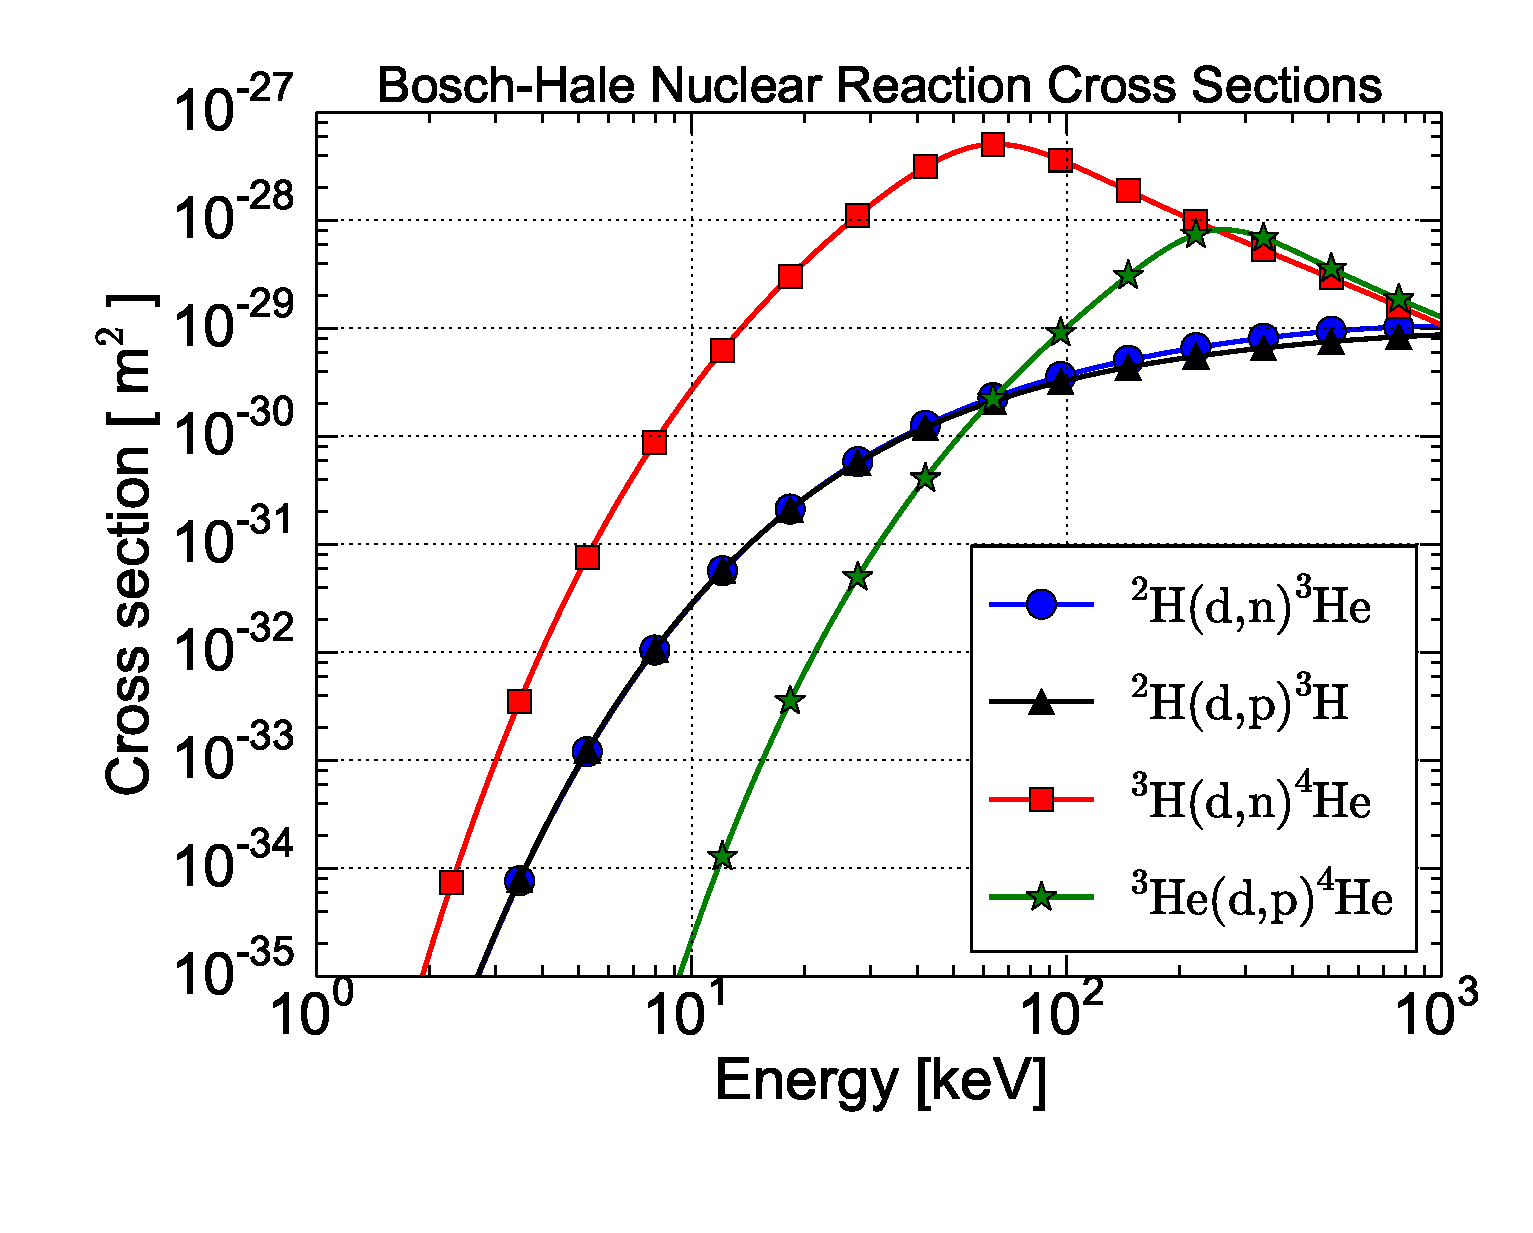
\includegraphics[width=0.95\columnwidth]{figures/BH_CrossSections.eps}
\end{figure}

\index{Reaction rates! Plotted data}
\noindent
\begin{figure}[hb!]
  \centering
  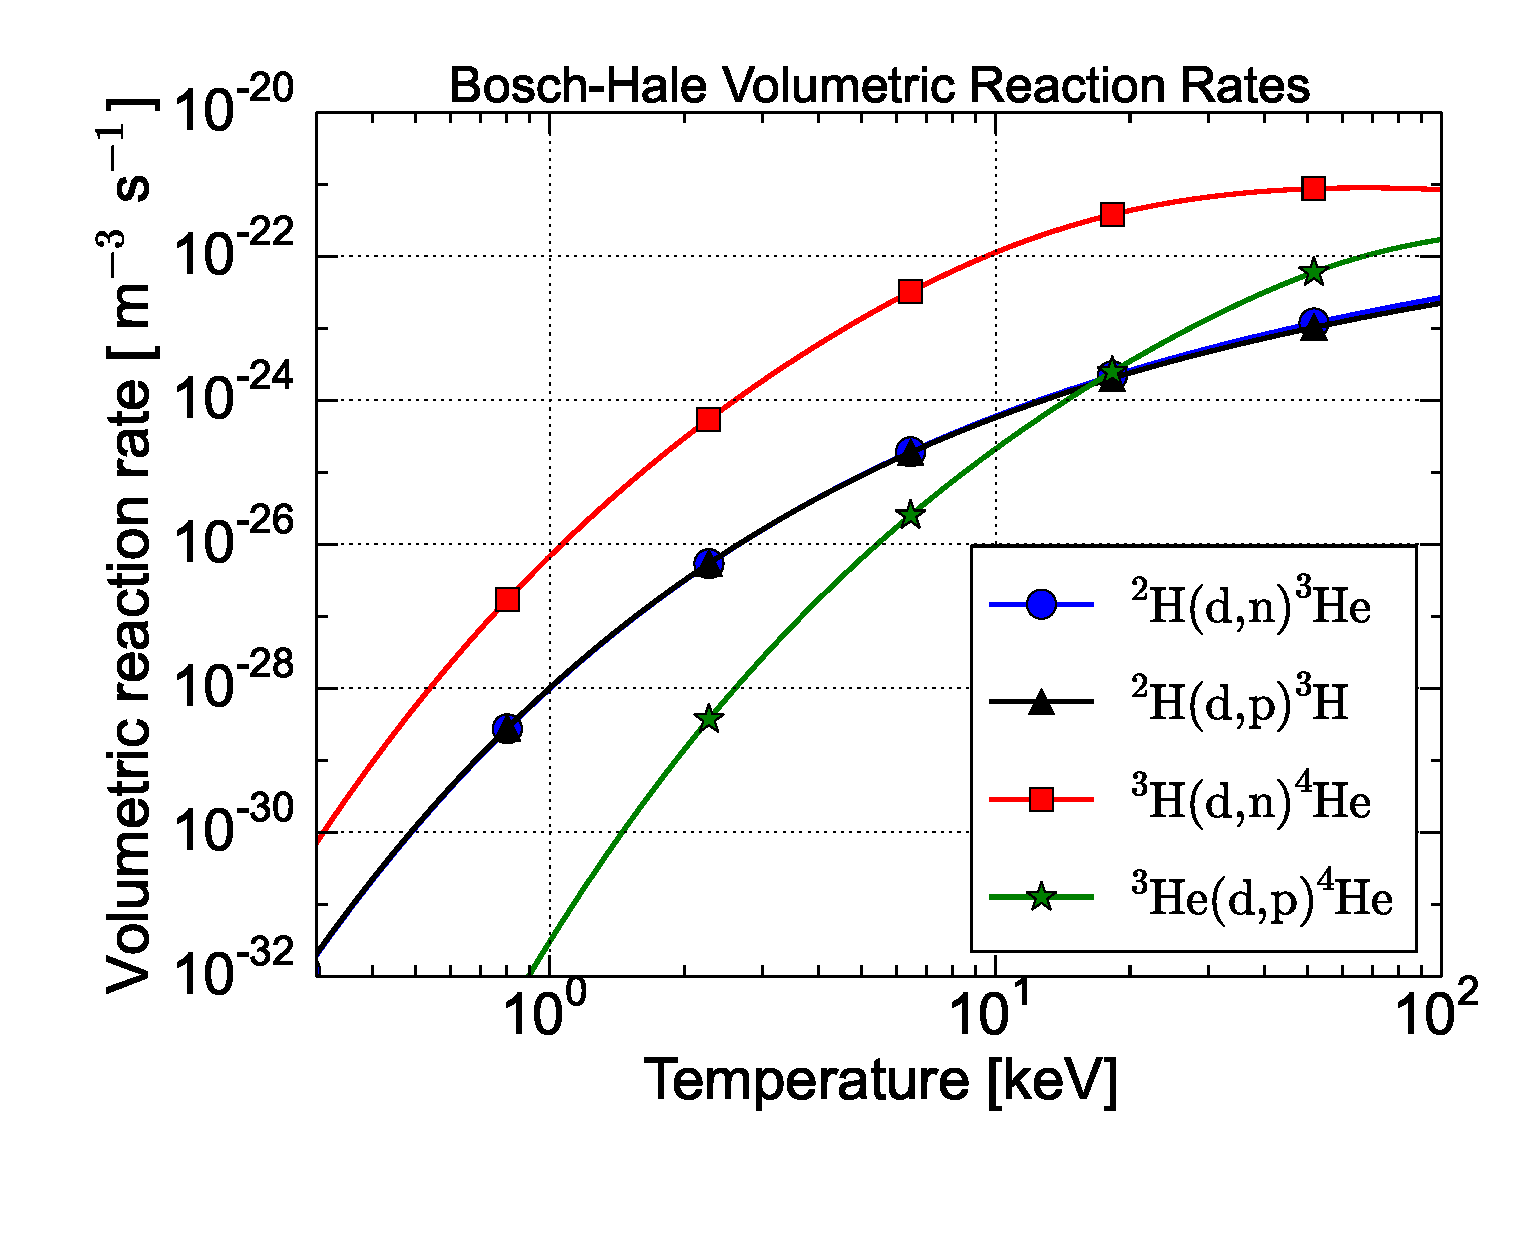
\includegraphics[width=0.95\columnwidth]{figures/BH_ReactionRates.eps}
\end{figure}

\vfill

\chapter{Tokamak Physics}
In this chapter, all units are SI with the exception of temperature,
which is defined in the historical units of eV (electron-volts).\\

\noindent
$e$ is the fundamental charge unit\\
$Z$ is the number of nuclear protons\\
$R_0$ is the major radius of a toroidal plasma\\
$a$ and $b$ are the horizontal and vertical minor radii of a toroidal plasma\\
\indent Note: $a=b$ for circular cross sections, and $a$ is used by convention\\
$R$ and $r$ denote lengths in the major and minor radii, respectively\\
$\theta$ and $\phi$ are the poloidal and toroidal angular coordinates, respectively\\
$B_x$ is the magnetic field in direction $x$\\
$B_{xa}$ is the magnetic field evaluated at the plasma edge in direction $x$\\
$I_p$ is the toroidal plasma current\\
$p$ is the plasma pressure\\
$v$ is velocity of the plasma\\

\section{Fundamental Definitions}

\index{$\epsilon$}
\index{Inverse aspect ratio}
\noindent
Inverse aspect ratio \scite{wesson}{117}
\fla{ \epsilon &= \frac{a}{R_0} &}

\index{Elongation}
\noindent
Plasma elongation \scite{wesson}{741}
\fla{\kappa &= \frac{b}{a} &}

\index{triangularity}
\noindent
Plasma triangularity \scite{wesson}{741}
\fla{\delta &= \frac{(c+d)/2}{a} &}
\indent where c, d are distances to the top of the plasma and the x-point, \\
\indent respectively, from the plasma center.\\

\index{Large aspect ratio expansion}
\noindent
Large aspect ratio expansion ($\epsilon \ll 1$) \scite{freidberg-PP}{280}
\fla{ \frac{1}{R} &\approx \frac{1}{R_0}\left(1-\frac{r}{R_0}\cos\theta\right) &}

\index{Surface area of a torus}
\noindent
Surface area of a torus 
\fla{ S_\mathrm{c-torus} &= 4\pi^2aR_0 &\hspace{0.5cm} \text{(Circular cross section) \scite{jeffrey}{24}}\\
      S_\mathrm{e-torus} &= 8\pi aR_0E(k) \approx 4\pi^2aR_0\left(\frac{1+\kappa^2}{2}\right)^{1/2} & \hspace{0.5cm} \text{(Elliptical cross section) \cite{wolfram}}}
\noindent

\index{Volume of a torus}
\noindent
Volume of a torus 
\fla{ V_\mathrm{c-torus} &= 2\pi^2a^2R_0 & \hspace{0.5cm} \text{(Circular cross section) \scite{jeffrey}{24}}\\
      V_\mathrm{e-torus} &= 2\pi^2a^2\kappa R_0 & \hspace{0.5cm} \text{(Elliptical cross section)} \cite{wolfram}}

\index{Toroidal plasma volume}
\noindent MHD toroidal plasma volume \scite{freidberg-MHD}{112}
\fla{V(\psi) &= \int\limits_{0}^{2 \pi} \! \int\limits_{0}^{2 \pi} \! \int\limits_{0}^{\hat{r}} \! R r dr d\theta d\phi & \\
 &= \pi R_{0} \int\limits_{0}^{2 \pi} \! d \theta \hat{r}^{2} \left[ 1 + \frac{2}{3} \left( \frac{\hat{r}}{R_{0}} \right) \cos \theta \right] \hspace{0.5cm} \text{ (low aspect ratio)}&}


\index{Plasma pressure}
\noindent
Volume averaged plasma pressure~~\cite{authors}
\fla{ \langle p \rangle &= \frac{1}{V}\!\!\!\!\int\limits_{volume}\!\!\!\! p\,d\tau &}

\index{Toroidal beta}
\noindent
Toroidal plasma beta \scite{freidberg-MHD}{71}
\fla{ \beta_t &= \frac{2\mu_0\langle p \rangle}{B_{\phi a}^2} &}

\index{Poloidal beta}
\noindent
Poloidal plasma beta \scite{freidberg-MHD}{71}
\fla{ \beta_p &= \frac{2\mu_0\langle p \rangle}{B_{\theta a}^2} = \frac{8\pi^2a^2 \kappa^{2}\langle p \rangle}{\mu_0 I_p^2} &}

\index{Radial electric field}
\noindent Radial electric field in a rotating toroidal plasma~~\cite{authors}
\fla{\textrm{E}_{r} &\approx \textrm{v}_{\phi} \textrm{B}_{\theta} - \textrm{v}_{\theta} \textrm{B}_{\phi} +\frac{1}{Z_{i} e n} \nabla p & }


%\subsection{Definitions of Plasma Beta in Pinches}
%\begin{table}[h!]
%  \begin{tabular}{l l}
%    \hline
%    Name & $\beta$\\
%    \hline\hline
%    $\theta$ pinch & $2 \mu_{0} <p>/B_{za}^{2}$\\
%    z pinch & $2 \mu_{0} <p>/B_{\theta a}^{2}$\\
%    Screw Pinch & $2 \mu_{0} <p>/\left( B_{za}^{2}+B_{\theta a}^{2} \right)$
%  \end{tabular}
%\end{table}

\section{Magnetic Topology}

\index{Toroidal magnetic field}
\noindent
Toroidal magnetic field for plasma confinement~~\cite{authors}
\fla{ B_\phi &\approx \frac{B_\phi(r)R_0}{R} &\\
  &\approx \frac{B_\phi(r)}{1-\epsilon\cos\theta} \text{  (valid for $\epsilon \ll 1$)} &}

\index{Poloidal magnetic field}
\noindent
Poloidal magnetic field for plasma confinement~~\cite{authors}
\fla{ B_\theta &\approx \frac{\mu_0 I_p(r)}{2\pi r} &}

\index{Safety factor}
\noindent
Safety factor (general) \scite{wesson}{111}
\fla{ q(r) &= \frac{\text{\# of toroidal field line orbits at r}}{\text{\# of poloidal field line orbits at r}} &\\}

\index{$q$, $q_*$}
\noindent
Safety factor for cylindrical plasma $(r,\theta,z)$ \scite{wesson}{112}
\fla{ q(r)_{\mathrm{cyl}}  &= \frac{rB_\phi(r)}{RB_\theta(r)} = \frac{2\pi r^2 B_\phi(r)}{\mu_0 I_p(r) R} &}

\noindent
Safety factor for toroidal plasma $(R,\theta,\phi)$ \scite{freidberg-PP}{288}
\fla{ q(r^*)_{\mathrm{tor}} &= \frac{1}{2\pi} \int\limits_0^{2\pi}\frac{rB_\phi}{RB_\theta}\,d\theta &\\
  &= \frac{r_0 B_\phi(r_0)}{R_0 B_\theta(r_0) \left(1 - r_0^2/R_0^2\right)^{1/2}} &}
\indent where the flux surfaces $r^*=r_0$ are circles.\\

\noindent
Safety factor at the edge for toroidal plasma $(R,\theta,\phi)$ \scite{freidberg-PP}{387}
\fla{ q_* &\equiv \frac{2\pi a^2 B_0}{\mu_0 R_0 I_{p}} = \frac{\pi k}{4 E(k) (\beta / \epsilon)^{1/2}} &}
\hangindent=0.25in where $E(k)\approx \left[ k^{2}+\pi^{2}/4(1-k^{2})\right]$ is the complete elliptic integral of the second kind and the definition of $k$ is given by
\fla{\frac{B_i^{2}}{B_{0}^{2}} & \equiv 1-\frac{2\mu_{0}p}{B_{0}^{2}} + \frac{4 \epsilon \mu_{0}p}{k^{2}B_{0}^{2}}\left( 2-k^{2} \right) &}

\noindent
Approximate edge safety factor for a large aspect ratio toroidal plasma \scite{freidberg-PP}{414}
\fla{q_{*} &\approx \frac{2 \pi B_{0}a^{2}}{\mu_{0}R_{0}I_{p}} \left( \frac{1+\kappa^{2}}{2}\right) &} %Freidberg 13.171

\index{Magnetic shear}
\noindent
Magnetic shear \scite{freidberg-PP}{408}
\fla{s &= \frac{r}{q}\frac{dq}{dr} &}


\section{Magnetic Inductance}

\index{Magnetic inductance}
\noindent
Definition of magnetic inductance \scite{freidberg-PP}{281}
\fla{ \frac{1}{2}LI^2 \, &\equiv \!\!\! \int \limits_\mathrm{volume} \!\!\! \frac{B^2}{2\mu_0}\,d\tau &}

\noindent
Normalized inductance per unit length [dimensionless] \scite{freidberg-PP}{281}
\fla{ \ell &\equiv \frac{L/2\pi R_0}{\mu_0/4\pi} = \frac{2L}{\mu_0 R_0} &}

\index{Inductance of plasma}

\index{Internal inductance}
\noindent
Internal inductance of a toroidal plasma \scite{freidberg-PP}{281}
\fla{ L_i &= \frac{8\pi R_{0}}{I_p^2} \int\limits_0^a \frac{B_\theta^2}{2\mu_0}\,r dr = \frac{\mu_0 R_0 \langle B_\theta^2 \rangle}{2B_{\theta a}^2} &\\
  \ell_i &= \frac{\langle B_\theta^2\rangle}{B_\theta^2(a)} &}

\index{External inductance}
\noindent
External inductance of a toroidal plasma \scite{freidberg-PP}{281}
\fla{ L_e &= \frac{8 \pi R_{0}}{I_p^2} \int\limits_a^\infty \frac{B_\theta^2}{2\mu_0}\,r dr = \mu_0 R_0\left(\ln \frac{8R_{0}}{a} - 2\right) &\\
  \ell_e &= 2\ln\frac{8R_{0}}{a} - 4 &}


\index{Toroidal force balance}
\section{Toroidal Force Balance}
\noindent
Equation of toroidal force balance \scite{freidberg-PP}{279}
\fla{ &\int \mathbf{\hat{R}} \cdot \left(\mathbf{J} \times \mathbf{B} - \nabla p\right)\,d\tau = 0 &}
\indent where
\fla{ \mu_0 \mathbf{J} &= \nabla \times \mathbf{B} = \frac{R_0}{R}\frac{\partial B_\phi}{\partial r}\mathbf{\hat{\boldsymbol{\theta}}} - \frac{1}{r}\frac{\partial}{\partial r}\left(\frac{R_0}{R}rB_\theta\right)\mathbf{\hat{\boldsymbol{\phi}}} &}
\fla{&\mathbf{\hat{R}} \cdot \mathbf{J} \times \mathbf{B} =& \\
  & -\cos\theta \left[\frac{R_0^2}{R^2}\frac{\partial}{\partial r}\left(\frac{B_\phi^2}{2\mu_0}\right)+\frac{R_0 B_\theta}{\mu_0 r R}\frac{\partial}{\partial r}\left(\frac{R_0}{R}rB_\theta\right)\right]-\frac{B_\mathrm{vert}}{\mu_0 r}\frac{\partial}{\partial r}\left(\frac{R_0}{R}rB_\theta\right) &}

\index{Hoop force}
\noindent
The hoop force\scite{freidberg-PP}{280}
\fla{ \mathbf{F_\mathrm{hoop}} &= \frac{I_p^2}{2}\frac{\partial}{\partial R}\left(L_i + L_e\right)\,\mathbf{\hat{R}} 
  = 2\pi^2a^2(\ell_i + \ell_e + 2)\frac{B_{\theta a}^2}{2\mu_0} \,\mathbf{\hat{R}} &\\
  &= \frac{\mu_0 I_p^{2}}{2}\left(\ln \frac{8R}{a} - 1 + \frac{\ell_i}{2}\right) \, \mathbf{\hat{R}}}

\index{Tire tube force}
\noindent
The tire tube force \scite{freidberg-PP}{280}
\fla{ \mathbf{F_\mathrm{tire}} &= 2\pi^2a^2\langle p \rangle \,\mathbf{\hat{R}} &\\
  &= \frac{\mu_0 I_p^2\beta_p}{4}\,\mathbf{\hat{R}}&}
%\indent where $\beta_p = (8\pi^2a^2\langle p \rangle)/(\mu_0 I_p^2)$ has been used.\\

\index{1/R force}
\noindent
The 1/R force \scite{freidberg-PP}{280}
\fla{ \mathbf{F_\mathrm{1/R}} &= 2\pi^2a^2\left(\frac{B_{\phi a}^2}{2\mu_0} - \frac{\langle B_\phi^2\rangle}{2\mu_0}\right) \,\mathbf{\hat{R}} &\\
  &= \frac{\mu_0 I_p^2}{4}\left(\beta_p -1\right)\,\mathbf{\hat{R}} &}
\indent where $\langle p \rangle = \frac{1}{2\mu_0}\left(B_{\phi a}^2 - \langle B_\phi^2 \rangle + B_{\theta a}^2\right)$\\
\indent have been used.\\

\noindent
The vertical field force on toroidal plasma ring \scite{freidberg-PP}{282}
\fla{ \mathbf{F_\mathrm{vert}} &= -2\pi R_0 B_\mathrm{vert}I_p \,\mathbf{\hat{R}}&}

\index{Vertical magnetic field}
\noindent
The vertical magnetic field required to balance toroidal forces \scite{freidberg-PP}{282}
\fla{ B_\mathrm{vert} &= \frac{\mathbf{F_\mathrm{hoop}}+\mathbf{F_\mathrm{tire}}+\mathbf{F_\mathrm{1/R}}}{2\pi R_0 I_p} &\\
  &= \frac{\epsilon}{4}B_{\theta a}\left(\ell_e + \ell_i + 2 + \frac{2\mu_0\langle p \rangle}{B_{\phi a}^2} + \frac{B_{\phi a}^2-\langle B_\phi^2\rangle}{B_{\theta a}^2}\right) &\\
  &= \frac{\mu_0 I_p}{4\pi R_0}\left(\ln\frac{8R}{a} - \frac{3}{2} + \frac{\ell_i}{2} + \beta_p\right) &}
\index{Shafranov shift}
Shafranov shift of the plasma center \scite{freidberg-MHD}{2129}

\fla{ \Delta &= \frac{b^2}{2 R_{0}} \left[ \left( \beta_{p} + \frac{l_{i} -1 }{2} \right) \left( 1 -\frac{a^{2}}{b^{2}} \right) + \ln \frac{b}{a} \right] - \frac{B_{vert}}{B_{\theta1}(b)}&}

\index{Paramagnetic plasmas}
\index{Diamagnetic plasmas}
\section{Plasma Para- and Dia-Magnetism}
Global pressure balance equation in a screw pinch  \scite{freidberg-PP}{270}
\fla{\langle p\rangle &= \frac{1}{2 \mu_{0}} \left( B_{za}^{2} - \langle B_{z}^{2} \rangle + B_{\theta a}^{2} \right) &}
\indent can be rearranged to give
\fla{\beta_{p} &= \frac{B_{za}^{2}-\langle B_{z}^{2} \rangle}{B_{\theta a}^{2}}+1 &}
\begin{align*}
  \indent 
  \mathrm{Diamagnetic:} & ~~\beta_{p} < 1 & \mathrm{Paramagnetic:} & ~~\beta_{p} > 1
\end{align*}


\section{MHD Stability Limits}
Using experimental data from a wide variety of tokamaks, empirical
scalings for critical tokamak instabilities have been constructed.
Units: current in MA, length in m, magnetic field in T, and density in
$n_{20} = n/10^{20}$.

\index{Troyon limit}
\index{Beta limit|see{Troyon limit}}
\begin{enumerate}
\item{Beta limits (no plasma shaping)
  \begin{flalign*}
    \beta_t &\le \beta_L\frac{I}{a B_\phi} & \\
    \beta_L &= 0.028 \text{  Troyon kink limit - no wall \cite{troyonlimit}} & \\
    \beta_L &= 0.044 \text{   Sykes ballooning limit - no wall} & \\
    \beta_L &= 0.06 \text{  kink - ideal conducting wall}  &
  \end{flalign*}
}
%\item{The Troyon (or beta) limit (plasma elongation $\kappa$)
%\fla{ \beta_t &\le 0.15\frac{\kappa \epsilon}{q_j} &}

%\noindent where $\epsilon = \frac{a}{R_0}$ and $q_j \approx 2\pi a^2 \kappa B_\phi/I_p R_0$
%}
\index{$\beta_{N}$}
\item{Definition of $\beta_{N}$ \scite{wesson}{347}
  \fla{\beta_{N} &\equiv \beta_{t} [\%] \,\frac{aB_{\phi}}{I_p \textrm{[MA]}} &}
}
  
\index{Greenwald limit}
\index{Density limit|see{Greenwald limit}}
\item{The Greenwald (or Density) Limit \scite{wesson}{377}
  \fla{ n_{20} \le n_G &= \frac{I_{p} \textrm{[MA]}}{\pi a^2} &}
}
\end{enumerate}

\section{Tokamak Heating and Current Drive}
\begin{enumerate}
\item{Ohmic plasma heating

\index{Ohmic heating}
The neo-classical resistivity approximation is \scite{freidberg-PP}{538}

\fla{ \eta_{||} &= \frac{1}{\left[1-(r/R_{0})^{1/2}\right]^{2}} \eta_{||}^{\textrm{Spitzer}} &}

\noindent Plugging in for the current as $J_{||}=E_{0}/\eta_{||}$ \scite{freidberg-PP}{539}

\fla{P_{\Omega} &= \left( \frac{5.6 \times 10^{-2}}{ 1-1.31 \epsilon^{1/2} + 0.46 \epsilon} \right) \left( \frac{R_{0} \left( I \textrm{[MA]} \right)^{2}}{a^2 \kappa T_{keV}^{3/2} } \right) \textrm{[MW]} &}
}

\item{Neutral beam plasma heating \scite{wesson}{246-248}

\index{Neutral beam heating}
%Neutral beams deposit their energy via collisions with the ions and electrons in the plasma. The energy deposition from the beam is then calculated to be

\fla{ P &= m_{b} \frac{n e^{4} \textrm{ln} \Lambda}{2 \pi \epsilon_{0}^{2} m_{b}^{2}} \left( \frac{2 m_{e}^{1/2} E_{b}}{ 3 (2 \pi)^{1/2} T_{e}^{3/2}} + \frac{m_{b}^{3/2}}{2^{3/2} m_{i} E_{b}^{1/2}} \right) &}

\indent where $E_{b}$ is the energy of the beam.

\noindent The critical beam energy when the ions and the electrons are heated equally by the beam is

\fla{E_{c} &= 14.8 \frac{A_{b}}{A_{i}^{2/3}} T_{e} &}
}
\end{enumerate}
\subsection{Current Drive}

\begin{enumerate}

\item{Inductive current

\index{Inductive current}
This current is driven via the central solenoid. The current distribution is 
calculated through the use of Faraday's law and $J_{||}=E_{0}/\eta_{||}$. 
Total current normally has to be measured in order to normalize the distrubition of
 current density.
}
\item{Bootstrap current

\index{Bootstrap current}
Bootstrap current is the self-generated current drive in the plasma from trapped and passing electrons in the plasma. 

The exact form of the bootstrap current density is given by \scite{freidberg-PP}{496}

\fla{j_{B} &= -4.71 q \left( \frac{R_{0}}{r} \right)^{1/2} \frac{T}{B_{0}} \left[ \frac{\partial n}{\partial r} +0.04 \frac{n}{T} \frac{\partial T}{\partial r} \right] &}

\noindent The total bootstrap fraction is given by \scite{freidberg-PP}{496}

\fla{f_{B} &\approx -1.18 \frac{\partial}{\partial r}(\textrm{ln} n + 0.04 \textrm{ln} T) / \frac{\partial}{\partial r}(\textrm{ln} r B_{\theta}) \left( \frac{r}{R_{0}} \right)^{1/2}\beta_{p} \sim \epsilon^{1/2} \beta_{p} &}
}
\item{Neutral beam current drive

\index{Neutral beam current drive}
By positioning a neutral beam in the tangential direction, it is
possible to drive both rotation and current. Neutral beam current
drive efficiency scales as (at $E_{b}=40 A_{b} T_{e}$) \cite{cordey}

\fla{I[\mathrm{A}]/P[\mathrm{W}] &\approx \frac{0.06 T_{e}}{n_{20} R Z_{b}}(1-Z_{b}/Z_{\mathrm{eff}}) &}
}

\item{Lower hybrid current drive

\index{LHCD}
Currently one of the most used current drive mechanisms is the lower
hybrid system. It launches a wave that Landau damps on the fast
electron population and preferentially drives electrons in one
direction. \scite{freidberg-PP}{623}

\fla{I[\mathrm{A}]/P[\mathrm{W}] &= 1.17/\left( n_{||}^{2} R_{0} n_{20} \right) &}

\noindent There exists an accessibility condition for the waves which forces an increase in the launched $n_{||}$ \scite{stix}{100}

\fla{n_{||}^{2} &> \left(S^{1/2} + \left| \frac{D^{2}}{P} \right| ^{1/2} \right)^{2} &}

\indent where S, P, and D are defined in Chapter \ref{chap:plasmawaves}.\\
\noindent Because LHCD relies on Landau damping, there is an additional
constraint on the $n_{||}$: Landau damping dominates at $n_{||}^{c}
\gtrsim 7.0/T_{\mathrm{keV}}^{1/2}$ \cite{granatstein}
}

\item{Fast Magnetosonic wave current drive
\index{Fast Magnetosonic wave CD}

Allows peaked on-axis profiles and has the following current drive efficiency \cite{cordey}

\fla{I[\mathrm{A}]/P[\mathrm{W}] &= 0.025 \frac{T_{\mathrm{keV}}}{n_{20} R_{0}} &}
}

\end{enumerate}

\section{Empirical Scaling Laws}

\subsection{Energy Confinement Time Scalings}

\index{Goldston scaling|see{Energy confinement scalings}}
\noindent
Goldston auxiliary heated tokamak scaling (l refers to the plasma size $\sim a$) \scite{wesson}{152}
\fla{\tau_{E} & \sim B_{p}^{2} l^{1.8}/ n T &}

\index{Energy confinement scalings}

\noindent
The ITER-89 L-Mode (ITER89-P) \scite{wesson}{740}
\fla{\tau_E &= 0.048 I_M^{0.85}R_0^{1.2}a^{0.3}\kappa^{0.5}\bar{n}_{20}^{0.1}B_0^{0.2}A^{0.5}P_M^{-0.5} \hspace{0.5cm}\mathrm{[s]} &}

\noindent % Ref:  ITER Physics Basis 1999 (pg 2206, Ch 2, eqn 24)
The ITER-98 L-Mode \cite{iter}
\fla{\tau_E &= 0.023 I_M^{0.96}B_{T}^{0.03}n_{19}^{0.40}M^{0.20}R^{1.83}\epsilon^{-0.06}\kappa^{0.64}P_{MW}^{-0.73} \hspace{0.5cm}\mathrm{[s]} &}

\noindent % Ref:  ITER Physics Basis 1999 (pg 2204, Ch 2, eqn 20)
The ITER-98 (IPB98[y,2]); ELMy H-mode \cite{iter}
\fla{\tau_E &= 0.0562 I_M^{0.93}B_{T}^{0.15}n_{19}^{0.41}M^{0.19}R^{1.97}\epsilon^{0.58}\kappa^{0.78}P_{MW}^{-0.69} \hspace{0.5cm}\mathrm{[s]} &}

\index{Lindear regime scaling}
%\noindent The ITER-98 L-mode confinement only holds above a critical density below which the neo-Alcator scaling is used; 
% this is a weird formula; cited in ITER phys. basis, but came from a Japanese tokamak. Not neo-Alcator.
\noindent Scaling for linear regime energy transport \cite{iter}
\fla{\tau_{E} &= 0.07 n_{20} q \kappa^{0.5}aR^2 \hspace{0.5cm} \text{[s]}&}

\noindent Critical density of linear to saturated regime \cite{iter}
\fla{n_{20} &= 0.65 A_{i}^{0.5}B_{T} q^{-1}R^{-1} &} 

\subsection{Plasma Toroidal Rotation Scaling}

% cite Rice et al.
\index{Rice scaling|see{Toroidal rotation scaling}}
\index{Toroidal rotation scalings}
Plasma toroidal rotation (Rice) scaling \cite{rice}
\fla{\Delta V_{tor} & \propto \Delta W/I_{p} &}

\noindent The 2010 multi-machine scaling database found that (with $v_{a}$ being the Alfv\'en speed) \cite{rice}
\fla{v/v_{a} &= 0.65 \beta_{T}^{1.4} q_{j}^{2.3}&}

\indent where $q_{j} =2 \pi \kappa a^{2} B/\mu_{0} R I_{p}$

\index{L-H mode power scalings}
\subsection{L-H Mode Power Scalings}
\noindent
The ITPA empirical scaling law for the L to H mode transition power threshold \cite{martin} % Y. Martin 2008
%\fla{P_{\text{L-H}} = 2.84 B_t^{0.82}n_e^{0.58}M^{-1}Ra^{0.81} \text{     [MW]} }
\fla{P_{\text{L-H}}\textrm{[MW]} &= 2.15 e^{\pm 0.107} n_{20}^{0.782 \pm 0.037} B_{\text{T}}^{0.772\pm 0.031} a ^{0.975 \pm 0.08} R^{0.999 \pm 0.101} &}

\index{Turbulence}
\section{Turbulence}

Fundamental definitions \scite{wesson}{422-424}
\flatwo{L_{n} &= n/\nabla n & L_{T} = T/\nabla T}{5}
\flatwo{b &= k_{\theta}^2 \rho_{i}^{2} & \eta_{j} = L_{nj}/L_{Tj}}{5}
\fla{\epsilon &= m_{j} v^{2}/2 T_{j} &}

\index{Diamagnetic drift velocity}
\noindent The diamagnetic drift velocity \scite{wesson}{420}
\fla{\textbf{v}_{dj} &= \frac{\textbf{B} \times \nabla p_{j}}{q_{j}n_{j} B^{2}} &}

\index{Diamagnetic drift frequency}
\noindent Diamagnetic frequency \scite{wesson}{421}
\fla{\omega_{*j} &= - \frac{k_{y} T_{j}}{e B n} \frac{dn}{dr} &}

\noindent Ion Larmor radius evaluated at the sound speed \cite{tynan}
\index{$\rho_{S}$}
\fla{\rho_{S} &\equiv c_{s}/\Omega_{i} &}

\noindent Normalized Larmor radius 
\index{$\rho_{*}$}
\fla{\rho_{*} &\equiv \rho_{S}/a &}

\subsection{General Drift Wave Turbulence}

Mixing length estimate \cite{tynan}
\fla{ \tilde{n}^{\textrm{rms}}/n_{0} &\sim 1/k_{\bot} L_{\textrm{n}} &}

\noindent Density fluctuations and plasma potential correlation \cite{tynan}
\fla{ \tilde{n}/n_{0} &\approx \left( e\tilde\phi/kT_{e} \right) \left( 1-i\delta \right)&}

\hangindent=0.25in where $\delta$ is the dissipation of the electron momentum to the background plasma.\\

\noindent Time averaged electrostatic turbulent flux of particles $\tilde{\Gamma}$, momentum $\overleftrightarrow{\mu}$, and heat $\tilde{Q}$ \cite{tynan}

\index{Turbulent flux of particles}
\fla{\tilde{\Gamma} &= - \frac{\langle \tilde{n} \nabla \tilde{\phi} \rangle \times \bar{\textbf{B}}}{\textrm{B}^2} + \langle \tilde{n} \tilde{v}_{||}\rangle \textbf{B}/\textrm{B}&}

\index{Turbulent flux of momentum}
\fla{\overleftrightarrow{\mu} &= \left\langle \left( -\frac{\nabla \tilde{\phi} \times \bar{\textbf{B}}}{\textrm{B}^{2}} + \tilde{v}_{||}\textbf{B}/\textrm{B} \right) \left( -\frac{\nabla \tilde{\phi} \times \textbf{B}}{B^{2}} + \tilde{v}_{||}\textbf{B}/\textrm{B} \right) \right\rangle &}

\index{Turbulent flux of energy}
\fla{\tilde{Q} &\equiv \frac{5}{2} \bar{n}\bar{T} \left[ \frac{1}{\bar{T}} \left( - \frac{\langle \tilde{T}\nabla \tilde{\phi} \rangle \times \bar{\textbf{B}}}{\textrm{B}^2}+ \langle \tilde{T}\tilde{v}_{||} \rangle \textbf{B}/\textrm{B} \right) + \frac{1}{\bar{n}} \left(  - \frac{\langle \tilde{n} \nabla \tilde{\phi} \rangle \times \bar{\textbf{B}}}{\textrm{B}^2} + \langle \tilde{n} \tilde{v}_{||}\rangle \textbf{B}/\textrm{B} \right) \right] &}


\indent where fluctuating values are marked by a tilde and $\langle ~ \rangle$ is a time average. \\

\noindent
Time averaged momentum and and energy fluxes due to fluctuating magnetic fields \cite{tynan}

\index{Magnetic turbulence flux of momentum}
\fla{\overleftrightarrow{\mu}^{EM} & = \frac{\langle \tilde{B}\tilde{B} \rangle}{\mu_{0} \bar{n} M_{i}} &}

\index{Magnetic turbulence flux of energy}
\fla{\tilde{Q}^{EM} &= \frac{\langle \tilde{q}_{||e} \tilde{B} \rangle }{\bar{B}} &}

\begin{figure}[h!]
\centering
  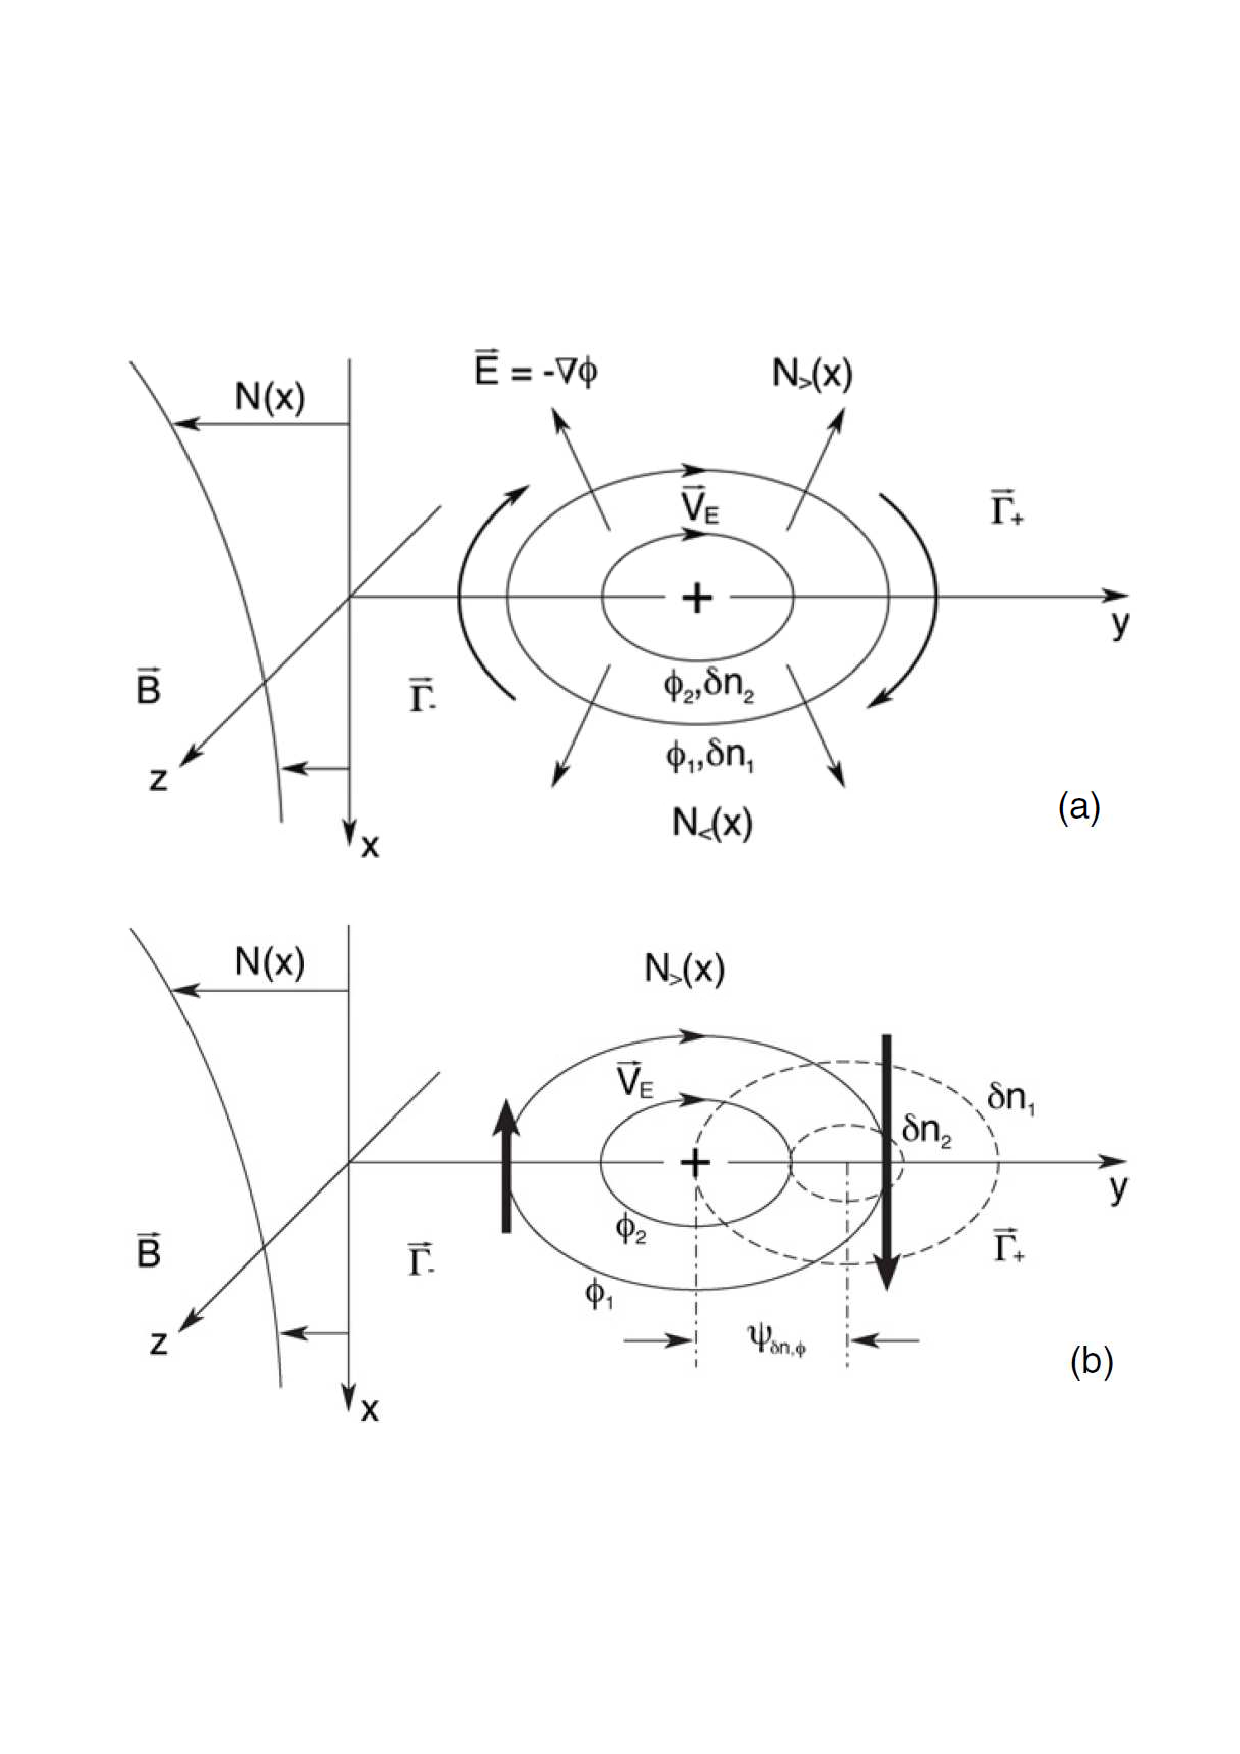
\includegraphics[scale=.5]{figures/turbulencefigure}
  \caption*{\small (a) Fluctuations without parallel electron dissipation. (b) Fluctuations with finite electron dissipation. Figure from Tynan et al 2009. Copyright 1999 by the American Physical Society.}
\end{figure}

\subsection{General Drift Turbulence Characteristics}

Perpendicular drift wave turbulence is characterized by $\rho_{S}$, with $k_{||} \ll k_{\bot}$ and $k_{\bot}\rho_{S}$ depending on dissipative mechanism, linear free energy source, and nonlinear energy transfer.\\

\index{Ion thermal gradient instability}

\noindent Ion thermal gradient (ITG) turbulence occurs when $\eta_{i} > \eta_{\textrm{crit}} \sim 1$ and has the following approximate characteristics \cite{tynan}
\fla{k_{\bot} \rho_{s} &\sim 0.1-0.5 &}
\fla{R/L_{T_{i}} &> R/L_{T_{i}}|_{\textrm{crit}} \sim 3-5 &}
\fla{v_{ph} &\sim v_{di} &}

\index{Trapped electron mode}
\index{Electron thermal gradient instability} 
\noindent Trapped electron mode (TEM) instabilities occurs at approximately $k_{\bot}\rho_{S} \sim 1$. At higher wavenumbers the TEM transitions into the electron thermal gradient (ETG) instability with $\eta_{e} > \eta_{\textrm{crit}} \sim 1$ and the following approximate characteristics \cite{tynan}
\fla{k_{\bot} \rho_{s} &\sim 1-10 &}
\fla{R/L_{T_{e}} &> R/L_{T_{e}}|_{\textrm{crit}} \sim 3-5 &}

\index{Passing particle modes}
\subsection{Passing Particle Instabilities}
In this section, it is assumed that $k_{||} v_{te}>> \omega >> k_{||}v_{ti}$, such that electrons respond to the electrostatic potential. Also, the frequency of the magnetic curvature drifts is assumed to be \scite{wesson}{422}
\fla{\omega_{di} &= 2 L_{n}\omega_{*i}/R \ll \omega &}

\index{Passing particle dispersion relation}
\noindent
The passing particle dispersion relation \scite{wesson}{424}
\fla{ \left[\rho_{i}^{2} \frac{\partial^{2}}{\partial x^{2}} - 
  \left(\frac{L_{n}/R}{b^{1/2} (T_{e}/T_{i}) q \Omega} \right)^{2}\left( \frac{\partial}{\partial \theta} + i k_{\theta} s x \right) - 
  \frac{2 R/L_{n}}{(T_{e}/T_{i}) \Omega} \left(\cos\theta +  \frac{i \sin\theta}{k_{\theta}} \frac{\partial}{\partial x} \right)\right. -&\\
  \left.\left(\frac{\Omega-1}{(T_e/T_i) \Omega + (1+\eta_i)} + b \right)\right] \tilde{\phi} &= 0 &}
\hangindent=0.25in where x is the distance from the reference mode rational surface $\textrm{m}=\textrm{n} q(\textrm{r})$ and $\tilde{\phi}$ is the perturbed electrostatic potential.\\

\index{Ion thermal gradient instability}
\index{ITG |see{Ion thermal gradient instability}}
\noindent
Ion thermal gradient (ITG, eta-i, $\eta_i$) toroidal frequency \scite{wesson}{428}
\fla{ \omega_\mathrm{ITG} &\approx (\eta_{i} \omega_{*i}\omega_{di})^{1/2} &}

\noindent
ITG critical instability limit \scite{wesson}{429}
\fla{ \eta_{ic} &= \left\{
\begin{gathered}
   1.2 \hspace{1cm}\hfill R/L_{n} < (R/L_{n})_{\textrm{crit}} \\
   \frac{4}{3} \left(1 + \frac{T_{i}}{T_{e}} \right) \left( 1 + 2s/q \right) R/L_{n}\hspace{1cm}\hfill  R/L_n > (R/L_n)_\mathrm{crit} \\
\end{gathered} \right. &}

\indent where
\fla{(R/L_{n})_{\textrm{crit}} &= \frac{0.9}{(1+T_{i}/T_{e})(1+2s/q)} &}


% ?????
% If $R/L_{n} < (R/L_{n})_{crit}$ then $\eta_{ic} = 1.2$

\index{Electron thermal gradient instability} 
\index{ETG|see{Electron thermal gradient instability}}
\noindent
Electron thermal gradient (ETG, $\eta_{e}$ mode) dispersion relation with $T_{i}\approx T_{e}$ \scite{wesson}{429}
\fla{-\frac{k_{||}^{2} v_{te}^{2}}{\omega^{2}} \left( 1- \frac{\omega_{*e}}{\omega} (1 + \eta_{e}) \right)+1 + \frac{\omega_{*e}}{\omega} &= 0 &} 

\indent If $\eta_{e} \gg 1$ then there is an unstable mode with \scite{wesson}{429}
$\omega \approx (-k_{||}^{2}v_{te}^{2} \eta_{e} \omega_{*e})^{1/3}$

\index{Trapped particle modes}
\subsection{Trapped Particle Modes}

\index{Trapped particle dispersion relation}
The collisionless trapped particle dispersion relation \scite{wesson}{432}
\fla{\frac{1}{\sqrt{2 \epsilon}} \left( \frac{1}{T_{i}} + \frac{1}{T_{e}} \right) &= \frac{1}{T_{i}} \frac{\omega-\omega_{*i}}{\omega-\bar{\omega}_{di}} + \frac{1}{T_{e}} \frac{\omega-\omega_{*e}}{\omega-\bar{\omega}_{de}} &}

\indent where 
\fla{\bar{\omega}_{dj} &= \frac{\omega_{dj}}{2} \left[ \left(\frac{v_{||}}{v_{Thj}} \right)^{2} + \left( \frac{v_{\bot}}{2 v_{Thj}} \right)^{2} \right] \{ \cos \theta + \frac{k_{r}}{k_{\theta}} \sin \theta \} &}

\index{Trapped ion mode}
\noindent This dispersion relation gives rise to the trapped ion mode if $\nu_{\textrm{eff}}=\nu_{j}/\epsilon > \omega_{dj}$ and has growth/frequency\scite{wesson}{433-434}
\fla{\omega &= \frac{\sqrt{2 \epsilon}}{1 + T_{e}/T_{i}} \omega_{*e} - i \frac{\nu_{i}}{\epsilon} + i \frac{\epsilon^2}{(1+T_{e}/T_{i})^2} \frac{\omega_{*e}^{2}}{\nu_{e}} &}

This mode has the largest imaginary part if $\nu_{e}\approx \epsilon^{3/2} \omega_{*e}$.\\

\index{Trapped electron mode}
\index{TEM|see{Trapped electron mode}}
\noindent
The TEM can be calculated due to the trapped particle dispersion
relation. The mode is driven by trapped electron collisions and
electron temperature gradients. \scite{wesson}{434-435}\\

\noindent If $\nu_{\textrm{eff}} \gg \omega_{*e}$ then the growth rate is 

\fla{\gamma &\approx \epsilon^{3/2} \frac{\omega_{*e}^{2}}{\nu_{e}} \eta_{e} &}

\begin{table}
  \centering
  \begin{tabular}{c c c c}
    \hline
    Parameter\T&  Approximate range          &  Approximate length &  Mode\\
             \B&  in $k_\theta$ (cm$^{-1}$) &  scale(cm)          & \\
    \hline\hline
    \multirow{5}{*}{Density fluctuations ($\tilde{n}$)}\T& $<$ 1              & 60       & ITG \\
                                  & $<$ 2              & 1        & ITG, TEM \\
                                  & $<$ 7              & 1-10     & ITG, TEM \\
                                  & 3-12 & 1        & TEM \\
                                  & $>$ 20             & 1, 20    & ETG \\
    Temperature fluctuations ($\tilde{T_e}$)                 & $<$ 1              & 1        & ITG \\
    Flows, GAMs, ZF               & $<$ 1              & 1        & ITG \\
    $\tilde{n_e}\tilde{T_e}$ cross phase    \B& $<$ 1              & 1        & ITG\\
    \hline
  \end{tabular}
\end{table}

\chapter{Tokamak Edge Physics}
In this chapter, all units are SI with the exception of temperature,
which is defined in the historical units of eV (electron-volts).\\

\noindent
$e$ is the elementary electric charge\\
$q$ is the total particle charge\\
$Z$ is the particle atomic (proton) number\\
$T$ is the plasma temperature\\
$n$ is the plasma number density\\
$p$ is the plasma pressure\\
$e$ and $i$ refer to electrons and ions, respectively\\
$a$ and $R_0$ are the minor and major radii of a toroidal plasma\\

\index{Scrape off layer (SOL)}
\section{The Simple Scrape Off Layer (SOL)}
The simple SOL model describes 1D plasma flow from the core plasma to
material boundary surfaces for limited or diverted plasma along the
toroidal magnetic topology.  By assuming a high degree of
collisionality ($\nu_*$), fluid approximations for plasma flow are valid
and the neoclassical effects on particle orbits due to toroidal
magnetic topology can be safely ignored.\\

\index{Connection length}
\noindent
Parallel SOL connection length (rail/belt limiters, poloidal divertors) \scite{stangeby}{17}
\fla{ L_{||} &\approx \pi Rq&}

\noindent
Particle time in the SOL (simple 1D model) \scite{stangeby}{20}
\fla{ t_\mathrm{dwell} &\approx L_\parallel / c_\mathrm{s} &}

\noindent
SOL width (simple 1D model) \scite{stangeby}{23}
\fla{ \lambda_\mathrm{SOL} &\approx \left(D_\perp L_\parallel / c_\mathrm{s}\right)^{1/2} &}
\indent where $D_\perp$ is the anomalous diffusion coefficient.\\

\noindent
Force balance / pressure conservation in the SOL \scite{stangeby}{47}
\fla{ p_\mathrm{e} + p_\mathrm{i} + mnv^2 &= \mathrm{constant} &}

\noindent
Plasma density variation along the SOL \scite{stangeby}{47}
\fla{ n(x) &= \frac{n_0}{1+M(x)^2} &}
\indent where $n_0$ is the density at the 'top' of the SOL and \\
\indent $M=v/c_s$ is the plasma mach number.\\

\noindent
Electrons follow a Boltzmann distribution in the SOL \scite{stangeby}{28}
\fla{ n &= n_0\mathrm{exp}\left(eV/T_\mathrm{e}\right) &}

\noindent
SOL particle sources: ionization (i) and cross-field transport (t) \scite{stangeby}{35-40}
\fla{S_\mathrm{p} &= S_\mathrm{p,i}+S_\mathrm{p,t} = n_\mathrm{plasma}n_\mathrm{neutrals}\langle\sigma v\rangle_\mathrm{i} + D_\perp n / \lambda_\mathrm{SOL}^2 &}
\indent
where $\langle\sigma v\rangle_\mathrm{i} \equiv \langle\sigma v\rangle_\mathrm{i}(T_\mathrm{e},Z)$ is the ionization rate coefficient.\\

\noindent
Particle flux density in the SOL at the sheath edge (se) \scite{stangeby}{47}
\fla{ \Gamma_\mathrm{se} &= \frac{1}{2}n_0c_\mathrm{s} &}
\indent where $n_0$ is the density outside the pre-sheath.\\

\noindent
Electric field through SOL required to satisfy the Bohm Criterion \scite{stangeby}{48}
\fla{ V_\mathrm{se} &= -0.7\frac{T_\mathrm{e}}{e} &}

\noindent
Floating sheath voltage \scite{stangeby}{79}
\fla{ V_\mathrm{s} &= 0.5\frac{T_e}{e}\ln\left[2\pi \frac{m_e}{m_i}\left(Z+\frac{T_i}{T_e}\right)\right] &} %Changed \left(2+\frac{T_i}{T_e}\right) to \left(Z+\frac{T_i}{T_e}\right)

\noindent
Debye sheath width \scite{stangeby}{27}
\fla{ \lambda_\mathrm{Debye} &\approx \left(\frac{\epsilon_0 T_\mathrm{e}}{n_\mathrm{e}e^2}\right)^{1/2} &}


\index{Bohm criterion}
\section{Bohm Criterion}
The Bohm Criterion is derived from conservation of energy
($1/2m_iv^2=-eV$) and particle conservation ($n_iv=constant$).  In an
unmagnetized plasma it sets the SOL plasma exit velocity into the
sheath edge (se). In magnetized plasma, it sets the SOL plasma exit
velocity parallel to the magnetic field, after which the ions become
demagnetized and perpendicularly enter the sheath; electrons remain
magnetized. \scite{stangeby}{61-98}.\\

\noindent
Bohm Criterion (assuming $T_i = 0$) \scite{stangeby}{73}
\fla {v_\mathrm{se} &\geq \left(\frac{T_e}{m_i}\right)^{1/2} \!\! = c_s &}

\noindent
Bohm Criterion (general form) \scite{stangeby}{76}
\fla{ \int \limits_0^{\infty} \frac{f_\mathrm{se}^i(v)\,dv}{v^2} &\leq \frac{m_i}{T_e} &\\}

\index{Two point model}
\section{A Simple Two Point Model For Diverted SOLs}
Diverted plasmas can obtain significant $\Delta$T along the SOL,
resulting in divertor temperatures less than 10 eV.  The SOL can be
approximated using a two point model: point 1 is the outboard midplane
entrance to the SOL (``upstream'' or ``u'') and point 2 is the
divertor terminus of the SOL (``target'' or ``t'').  It is assumed
that upstream density, $n_u$, and the heat flux into the SOL,
$q_{||}$, are control parameters; upstream and target temperatures,
$T_u$ and $T_t$, as well as plasma density in front of the target,
$n_t$, are subsequently determined.

\subsection{Definitions}

\noindent
Dynamic and static pressure \scite{stangeby}{435}
\fla{ p &= nT\left(1+M^2\right) \hspace{0.5cm}\mathrm{where}\hspace{0.5cm} \left\{
  \begin{gathered}
    M_\mathrm{u}^2 \ll 1\\ %Changed \gg to \ll
    M_\mathrm{t}^2 \approx 1~\text{(Bohm Criterion)}\\
  \end{gathered} \right. 
  &
}

\index{Heat conduction}
\noindent
Heat conduction parallel to magnetic field \scite{stangeby}{187}
\fla{ q_{\parallel,~\mathrm{cond}} &= -k_0T^{5/2}\frac{dT}{dx} \hspace{0.5cm}\mathrm{where}\hspace{0.5cm} \left\{
  \begin{gathered}
    k_\mathrm{e,0} \approx 2000~~\mathrm{[W~m^{-1}~eV^{7/2}]}\\
    k_\mathrm{i,0} \approx 60~~\mathrm{[W~m^{-1}~eV^{7/2}]}\\
  \end{gathered} \right.
  &
}

\index{Heat flux tranmission coeficient}
\noindent
Sheath heat flux transmission coefficient at a biased surface \scite{stangeby}{652}
\fla{ \gamma &= 2.5\frac{T_i}{ZT_e}-\frac{eV}{T_e}+2\left[2\pi\frac{m_e}{m_i}\left(Z+\frac{T_i}{T_e}\right)\right]^{-1/2}\exp\left(\frac{eV}{T_e}\right) + \chi_i &}
\indent where $T_e\neq T_i$, $\chi_i$ is the electron-ion recombination energy,\\
\indent and no secondary electrons emitted.\\


 %Changed 2\left[\left(Z+\frac{T_i}{T_e}\right)2\pi\frac{m_e}{m_i}\right]^{1/2} to 2\left[2\pi\frac{m_e}{m_i}\left(Z+\frac{T_i}{T_e}\right)\right]^{-1/2}

\subsection{Fundamental Relations}
\noindent
SOL pressure conservation \scite{stangeby}{224}
\fla{ 2n_tT_t &= n_uT_u&}

\noindent
SOL power balance \scite{stangeby}{224}
\fla{ T_u^{7/2} &= T_t^{7/2} + \frac{7q_{||}L}{2 k_0 } &}

\noindent
SOL heat flux limited to sheath heat flux \scite{stangeby}{224} 
\fla{ q_{||} &= \gamma n_t T_t c_{st} &
             &\approx 7 \hspace{0.5cm} \text{(D-D plasma, floating surface)} &}

\subsection{Consequences}
\noindent
Upstream SOL temperature \scite{stangeby}{226}
\fla{ T_u &\approx \left(\frac{7q_{||}L}{2k_0}\right)^{2/7} \hspace{0.5cm} \text{assuming that } T_t^{7/2} \ll T_u^{7/2} &}
\indent
$\rightarrow T_u$ is independent of $n_u$\\
\indent
$\rightarrow T_u$ is insensitive to parameter changes due to the 2/7 power\\
\indent
$\rightarrow q_\parallel$ is extremely sensitive to $T_u$ due to the 7/2 power\\

\noindent
Target SOL temperature \scite{stangeby}{227}
\fla{ T_t &\approx \frac{2m_i}{\gamma^2e^2}\, \frac{q_\parallel^{10/7}}{(Lk_0)^{4/7}n_u^{2}} &}
\indent
$\rightarrow T_t$ is proportional to $\frac{1}{n_u^2}$\\

\noindent
Target SOL density \scite{stangeby}{227}
\fla{ n_T &= \frac{n_u^3}{q_{||}^2}\left(\frac{7q_{||}L}{2k_0}\right)^{6/7}\frac{\gamma^2 e^2}{4m_i}  &}
\indent
$\rightarrow n_T$ is proportional to $n_u^3$

\chapter{Tokamak Fusion Power}
In this chapter, all units are SI with the exception of temperature
and energy, which are defined in the historical units of eV
(electron-volts).\\

\noindent
$n$ is the plasma density; $n_{20}=n/10^{20}$; $n_0 = n_e \approx n_i$\\
$T$ is the plasma temperature; $T_\mathrm{keV}$ = $T$ in units of kiloelectron-volts\\
$p$ is the plasma pressure\\
$\nu$ is the radialprofile peaking factor\\
$P$ is a power density\\
$S$ is a total power\\
$U$ is a total energy\\
$E$ is the nuclear reaction energy gain\\
$e$ is the elementary electric charge\\
$q$ is the total particle charge\\
$Z$ is the particle atomic (proton) number\\
$e$ and $i$ subscripts refer to electrons and ions, respectively\\
$D$ and $T$ refer to deuterium and tritium, respectively\\
$\kappa$ is the plasma elongation; $\kappa$=b/a\\
$a$,$b$, and $R_0$ are the 2 minor and major radii of a toroidal plasma\\
$V$ is the volume of the plasma\\

\section{Definitions}
\index{Power densities}
\noindent
Fusion power density \scite{wesson}{8}
\fla{P_\mathrm{fusion} &= n_D n_T \langle\sigma v\rangle_{DT} E_\mathrm{fusion} = \frac{1}{4}n_e^2\langle\sigma v\rangle_{DT} E_\mathrm{fusion} &}

\noindent
Fusion power \scite{wesson}{22}
\fla{S_\mathrm{total} &= \frac{\pi}{2}E_\mathrm{fusion} \!\!\int \limits_{\substack{plasma\\ cross \\ section}}\!\! n^2\langle\sigma v\rangle_{DT} R\,dS & \\
                      &= \frac{0.15}{2\nu +1}Rab\left(\frac{n}{10^{20}}\right)^2T_\mathrm{keV}^2 \hspace{0.5cm} \hspace{0.5cm} \mathrm{[MW]} &}
\indent
where it has been assumed that:
\begin{eqnarray*}
  &\text{Pressure profile: }& nT = \hat{n}\hat{T}\left(1-\frac{r^2}{\tilde{a}^2}\right)^\nu \\
  &\text{Reaction rate: }& \langle\sigma v\rangle_\mathrm{DT} \approx 1.1\times10^{-24}T_\mathrm{keV}^2 \\
  &\text{Plasma cross section: }& \tilde{a} = (ab)^{1/2}
\end{eqnarray*}

\noindent
Alpha power density \scite{wesson}{10}
\fla{P_\mathrm{\alpha} &= n_D n_T \langle\sigma v\rangle_{DT} E_\alpha = \frac{1}{4}n_e^2\langle\sigma v\rangle_{DT} E_\alpha  \approx (1/5)P_\mathrm{fusion}&}

\noindent
Neutron power density \scite{wesson}{10}
\fla{P_\mathrm{neutron} &= n_D n_T \langle\sigma v\rangle_{DT} E_\mathrm{neutron} = \frac{1}{4}n_e^2\langle\sigma v\rangle_{DT} E_\mathrm{neutron} \approx (4/5)P_\mathrm{fusion}&}

\noindent
Ohmic heating power density \scite{wesson}{240}
\fla{P_\mathrm{ohmic} &\approx \eta J_\mathrm{plasma}^2 &}

\index{Stored plasma energy}
\noindent
Stored energy in confined plasma \scite{wesson}{9}
\fla{ W &= \int 3nT\,d\tau = 3\langle nT\rangle V &}

\index{Energy confinement time}
\noindent
Definition of energy confinement time \scite{wesson}{9}
\fla{ \tau_E &= \frac{\text{Stored energy in the confined plasma}}{\text{Power lost from the confined plasma}} = \frac{W}{S_\mathrm{loss}} &}

\index{Conduction power losses}
\noindent
Power loss from a confined plasma due to conduction \scite{wesson}{9-10}
\fla{P_\mathrm{conduction} &= \frac{3nT}{\tau_E} &}

\index{Bremsstrahlung power losses}
\noindent
Power loss from a confined plasma due to bremsstrahlung radiation \scite{wesson}{227-228}
\fla{P_\mathrm{bremsstrahlung} &\approx (5.35\times10^{-37})Z^2 n_e n_i T_\mathrm{keV}^{1/2} \hspace{0.5cm} \text{[W m$^{-3}$]}  &}


\index{Power balance}
\section{Power Balance in a D-T Fusion Reactor}
Confined fusion plasmas are not in thermal equilibrium, and,
therefore, power must be balanced in a steady-state tokamak reactor.
Power that is lost from the confined plasma due to conduction,
radiation and other mechanisms must be continuously replenished by
alpha particle and auxilliary heating mechanisms.

\noindent
\fla{ 0 &= \left(P_{\mathrm{alpha}} + P_{\mathrm{auxilliary}}\right) - \left(P_{\mathrm{conduction}} + P_{\mathrm{bremsstrahlung}} + \ldots\right) &}
\indent 
where 
\fla{\indent &P_{\mathrm{auxilliary}} = P_{\mathrm{ohmic}} + P_{\mathrm{ICH}} + P_{\mathrm{ECH}} + P_{\mathrm{neutral~beam}} + \ldots &}

\subsection{Impurity Effects on Power Balance}
The fractional impurity densities $f_j=n_j/n_0$ in the plasma core cause:
\begin{enumerate}
  \item{Modified quasi-neutrality balance \scite{wesson}{36}
    \fla{ n_e &= n_D + n_T + \sum\limits_jZn_j &}}
  \item{Increased radiated power loss~~\cite{authors}
    \fla{ P_{\mathrm{bremsstrahlung}} &\approx (5.35\times10^{-37})n_e^2T_\mathrm{keV}^{1/2}Z_\mathrm{eff} \hspace{0.5cm} \text{[W m$^{-3}$]} &}}
  \item{Dilution of fusion fuel~~\cite{authors}
    \fla{ P_{\mathrm{alpha}} &= \frac{1}{4}n_e^2(1-\sum\limits_jf_jZ_j)^2\langle\sigma v\rangle E_\alpha &}}
\end{enumerate}

\index{Q! Fusion}
\subsection{Metrics of Power Balance}

\index{Physics gain factor}
\noindent
The physics gain factor for D-T plasma \scite{wesson}{12}
\fla{ Q_\mathrm{phys} &= \frac{\frac{1}{4}n_e^2\langle\sigma v \rangle E_\mathrm{fusion} \cdot V_{\mathrm{plasma}}}{P_{\mathrm{heating}}} = \frac{5P_\alpha}{P_{\mathrm{heating}}} &}
\indent
where
\begin{enumerate}
  \item{$Q_\mathrm{phys}$=1 is break even}
  \item{$Q_\mathrm{phys}>$5 is a burning plasma}
  \item{$Q_\mathrm{phys}=\infty$ is an ignited plasma}
\end{enumerate}

\index{Engineering gain factor}
\noindent
The engineering gain factor~~\cite{authors}
\fla{ Q_\mathrm{eng} &= \frac{P_\mathrm{electricity}^\mathrm{out}}{P_\mathrm{electricity}^\mathrm{in}} &}


\index{Ignition condition}
\index{Lawson criterion|see{Ignition condition}}
\section{The Ignition Condition (or Lawson Criterion)}
The ignition condition describes the minimum values for density ($n$),
temperature ($T$), and energy confinement time ($\tau_E$) that are
required for a confined plasma to reach ignition.  Ignition is defined
as $P_\mathrm{alpha} > P_{\mathrm{loss}}$, where
$P_{\mathrm{auxilliary}} = 0$. \scite{wesson}{10-15} For a given
temperature, $T$, the following equations describe the minimum
$n\tau_E$ required to reach ignition under different assumptions:

\begin{enumerate}

   \item{$P_\mathrm{alpha} = P_\mathrm{conduction}$ \scite{wesson}{10-11}
     \fla{n\tau_E &= \frac{12kT}{\langle\sigma v\rangle E_\alpha} &}
    Using $\langle\sigma v\rangle_{DT} \approx 1.1\times10^{-24}T_\mathrm{keV}^2$
    and $E_\alpha = 3.5 \,\mathrm{MeV}$~~\cite{authors}:
    \fla{nT\tau_E &\gtrsim 3\times10^{21} \text{ m$^{-3}$ keV s} &}}

  \item{$P_\mathrm{alpha} = P_\mathrm{conduction} + P_\mathrm{bremsstrahlung}$~~\cite{authors}: 
     \fla{n\tau_E &= \frac{12kT}{\langle\sigma v\rangle E_\alpha - 2.14\times10^{-36}T_\mathrm{keV}^{1/2}} &}}

  \item{$P_\mathrm{alpha} = P_\mathrm{conduction} + P_\mathrm{bremsstrahlung}$ with alpha impurities $f_\alpha = n_\alpha/n_e$~~\cite{authors}: 
    \fla{n\tau_E &= \frac{12kT}{(1-2f_\alpha)^2\langle\sigma v\rangle E_\alpha - (1+2f_\alpha)2.14\times10^{-36}T_\mathrm{keV}^{1/2}} &}}

  \item{$P_\mathrm{alpha} = P_\mathrm{conduction} + P_\mathrm{bremsstrahlung}$ with impurity densities $f_j = n_j/n_e$~~\cite{authors}:
    \fla{n\tau_E &= \frac{12kT}{(1-\sum\limits_jf_jZ_j)^2\langle\sigma v\rangle E_\alpha - (2.14\times10^{-36})Z_\mathrm{eff}T_\mathrm{keV}^{1/2}} &}}

\end{enumerate}

\chapter{Tokamaks of the World}

\index{Alcator C-Mod}
\index{ASDEX-U}
\index{DIII-D}
\index{EAST}
\index{FTU}
\index{Ignitor}
\index{ITER}
\index{JET}
\index{J-TEXT}
\index{JT-60SA}
\index{KSTAR}
\index{SST-1}
\index{T-10}
\index{T-15U}
\index{TCV}
\index{TEXTOR}
\index{Tore Supra}
\index{TFTR}
\index{NSTX-U}

\begin{itemize}

\item{Comprehensive list of all major tokamaks with parameters \\ \url{www.tokamak.info}}

\item{ASDEX-U \scriptsize(Garching, Germany)\\
  \url{http://www.ipp.mpg.de/ippcms/eng/for/projekte/asdex/techdata.html}}

\item{Alcator C-Mod \scriptsize(Cambridge, USA)\\ 
  \url{http://www.psfc.mit.edu/research/alcator/}}

\item{DIII-D \scriptsize(San Diego, USA)\\
  \url{https://fusion.gat.com/global/Home}}
%FST October 2005 issue
\item{EAST \scriptsize(Hefei, China)\\
  \url{http://english.hf.cas.cn/ic/ip/east}}
%EAST results paper for approximate 
\item{FTU \scriptsize(Frescati, Italy)\\
  \url{http://www.efda.org/eu\_fusion\_programme/machines-ftu\_i.htm}}

\item{Ignitor \scriptsize(Kurchatov, Russia)\\
  \url{http://www.frascati.enea.it/ignitor}}
  
\item{ITER \scriptsize(Cadarache, France)\\
  \url{http://www.iter.org/mach}}
  
\item{JET \scriptsize(Culham, United Kingdom)\\
  \url{http://www.jet.efda.org/jet/jets-main-features}}
  
\item{J-TEXT \scriptsize(Wuhan, China)\\
  \url{http://www.jtextlab.com/EN/SortInfo.aspx?sid=43}}
  
\item{JT-60SA \scriptsize(Naka, Japan)\\ 
  \url{http://www-jt60.naka.jaea.go.jp/english/figure-E/html/figureE\_jt60sa\_5.html}}
  
\item{KSTAR \scriptsize(Daejeon, S. Korea)\\
  \url{http://www.pppl.gov/kstar/html/about\_kstar.html}}

\item{NSTX-U \scriptsize(Princeton, USA)\\
  \url{http://nstx-u.pppl.gov/}}
  
\item{SST-1 \scriptsize(Gandhinagar, India)\\
  \url{http://www.ipr.res.in/sst1/SST1parameters.html}}
  
\item{T-10 \scriptsize(Kurchatov, Russia)\\}
  
\item{T-15U \scriptsize(Kurchatov, Russia)\\
  \url{www.toodlepip.com/tokamak/t15-ft\_p7-3.pdf}}
  
\item{TCV \scriptsize(Lausanne, Switzerland)\\
  \url{https://crppwww.epfl.ch/tcv}}
  
\item{TEXTOR \scriptsize(J\"{u}lich, Germany)\\
  \url{http://www2.fz-juelich.de/ief/ief-4//textor\_en}}
  
\item{TFTR \scriptsize(Princeton, USA)\\
  \url{http://w3.pppl.gov/tftr/info/tftrparams.html}}
  
\item{Tore Supra \scriptsize(Cadarache, France)\\
    \url{http://www-fusion-magnetique.cea.fr/gb/index.html}}

\end{itemize}
\vfill


\begin{sidewaystable}[ht]\footnotesize
  \centering
  \begin{tabular}{l c c c c c c c c c c c c c c c}
    \hline
    Tokamak\T&  R  &  a  &  $\epsilon$  &  B$_\mathrm{\phi}$\footnote{\scriptsize Magnet coils are conducting unless denoted as superconducting (SC)} &  I$_\mathrm{p}$  &  $\kappa$  &  $\delta$  &  V$\mathrm{p}$  &  Pulse   &  Config\footnote{\scriptsize Plasma configuration: L = limited; SN = diverted single null; DN = diverted double null}  &  PFC\footnote{\scriptsize Plasma Facing Components: Be = beryllium; C = CFC/graphite; Li = lithium; M = molybdenum; SS = stainless steel; W = tungsten}  &  ICRH  &  ECRH  & LHCD  &  Beam \\
           \B& (m) & (m) &              &  (T)                                                                                                  &  (MA)            &            &            &  (m$^{-3}$)     &  (s)     &                                                                                        &                                                                                                                                                                &  (MW)  &  (MW)  & (MW)  &  (MW) \\
    \hline\hline

    ASDEX-U \T\B& 1.65 & 0.5 & 0.30 & 3.1 & 1.4 & 1.8 & 0.4 & 14 & 10& SN & C/W & 6 & 4 & -& 20 \\    

    \rowcolor[gray]{0.9}
    C-Mod   \T\B& 0.67 & 0.22 & 0.33 & 8 & 2 & 1.7 & 0.6 & 1.0 & 2.5 & L/SN/DN & M & 6 & - & 1 &-\\

    DIII-D  \T\B& 1.66 & 0.67 & 0.40 & 2.2 & 3 & 2.6& 1.0&12 &5 & SN/DN & C & 5 & 6 & - & 20\\ % 12m^{3} approximate
    
    \rowcolor[gray]{0.9}
    EAST    \T\B& 1.70 & 0.40 & 0.24 & 3.5 SC & 0.5 & 2 & 0.5 & 13 & 1000 & DN/SN & C & 3 & 0.5 & 4 &-\\

    %\rowcolor[gray]{0.9}
    FTU     \T\B& 0.93 & 0.3 & 0.32 & 8 & 1.6 & 1.7 & 0.55 & 3  & 1.5 & L & SS/M/W & 0.5 & 1.3 & 2.5 & -\\ % k, d from Possible high-beta experiments in FTU D-shaped plasmas

    \rowcolor[gray]{0.9}
    Ignitor\footnote{\scriptsize Proposed; construction not begun} \T\B& 1.32 & 0.47 & 0.36 & 13& 11& 1.83& 0.4&11 & 10 & L & M & (18-24) & - & - & -\\

    ITER\footnote{\scriptsize Construction begun; first plasma predicted 2019} \T\B&  6.2 & 2 & 0.32 & 5.3 SC & 17 & 1.86 & 0.5 & 837 & 400 & SN & Be/C/W & 20 & 20 & - & 33\\

    \rowcolor[gray]{0.9}
    JET     \T\B& 2.96 & 0.96 & 0.32 & 3.8 & 5  & 1.7 & 0.33 &200 & 92& L/SN/DN& Be/W&- &7 & -&34\\    

    JT-60SA\footnote{\scriptsize Construction begun: first plasma predicted 2014}\T\B& 3.16& 1.02 & 0.32 & 2.7 SC& 5.5&1.83 & 0.57& 132& 100 & DN & C & -& 7& -&34\\

    \rowcolor[gray]{0.9}
    J-TEXT  \T\B& 1.05 & 0.26 & 0.25 & 3& 0.4 &1 &- &1.4 &0.3 & L/SN/DN &C &- & -&- &-\\ % taking circular plasma from TEXT-U

    KSTAR   \T\B&  1.8 & 0.5 & 0.28 & 3.5 & 2.0  & 2.0 & 0.8 &18 & 20 & DN & C & 6 & - & 1.5 & 8\\    

    \rowcolor[gray]{0.9}
    NSTX-U  \T\B&  0.93 & 0.57 & 0.61 & 1.0 & 2.0  & 2.5 & 0.3 & 15 & 5 & SN/DN & C/Li & 3  & 0.35 & - & 10\\    

    SST-1\footnote{\scriptsize Construction begun: first plasma predicted 2012} \T\B&  1.1 & 0.2 & 0.18 & 3C& 0.22 & 1.9& 0.8&2 & 1000 & DN & C & 1.5 & 0.2 & 1 & 0.8\\
    
    \rowcolor[gray]{0.9}
    T-10    \T\B&  1.5 & 0.36 & 0.24 & 5& 0.8 & 1& - &4 &1 &L & SS/C & - & 2 & - & -\\ % 30th, conference on Contr. Fusion and plasma Phys July 2003

    T-15    \T\B& 2.43 & 0.42 & 0.17 & 3.5 SC &1 & 1.47& 0.25& 12 & 1000& SN & C & -& 7& 4&9\\ % Superconducting Tokamak T-15 upgrade 

    \rowcolor[gray]{0.9}
    TCV     \T\B& 0.88 & 0.25 & 0.28 & 1.4 & 1.2  & 2.8 & -0.7--1 & 3 & 4 & L/SN/DN & SS/C & - & 4.5 & - & - \\

    Textor \T\B&  1.75 & 0.47 & 0.27 &2.8 &0.8 & 1& -&8 & 10&L/SN & SS/C & 4& 1& -&4\\

    \rowcolor[gray]{0.9}
    TFTR\footnote{\scriptsize Decommissioned in 1997}  \T\B&  2.52 & 0.87 & 0.35 & 5.6 &2.7  &1 & -&6 & 10 &L & C & 12.5 & - & - &39.5\\

    Tore Supra \T\B& 2.25 & 0.7 & 0.31 & 4.5 SC & 1.7 &1 & -&22 & 390 & L& C & 9 & 2.4 & 5 &1.7\\
    \hline
  \end{tabular}
\end{sidewaystable}




\backmatter

\renewcommand\bibname{References}
\bibliographystyle{plainnat}
\bibliography{MFEFormulary}

% Add the References section to the table of contents
\addcontentsline{toc}{chapter}{References}

% Bit of a hack required to add the Index section to the table of contents
\cleardoublepage
\phantomsection
\addcontentsline{toc}{chapter}{Index}
\printindex


\end{document} 
